\documentclass[a4paper,12pt,twoside]{book}
\usepackage[T1]{fontenc}
\usepackage{inputenc}
\usepackage{fontspec}
\usepackage{lmodern}
\usepackage[english,french]{babel}
\usepackage{xspace} % Pour la gestion des espaces après les commandes
\usepackage{csquotes} % Gestion des guillemets dans la biblio et citations
\usepackage[xetex]{graphicx} % Package pour gérer les images
\usepackage{caption}
\usepackage{subcaption} % Package pour les subfigures
\usepackage{float} % Gestion de la position des images
\usepackage{listings} % Blocs de code
\usepackage{xcolor} % Couleurs des blocs de code
\usepackage{pdfpages} % Insertion de PDF dans le fichier

% Couleurs des blocs de code
\definecolor{ferngreen}{rgb}{0.31, 0.47, 0.26}
\definecolor{codegray}{rgb}{0.44, 0.5, 0.56}
\definecolor{sinopia}{rgb}{0.8, 0.25, 0.04}
\definecolor{silver}{rgb}{0.95, 0.95, 0.95}
\definecolor{bondiblue}{rgb}{0.0, 0.58, 0.71}

%Style des blocs de code
\lstdefinestyle{code-memoire}{
	backgroundcolor=\color{silver},   
	commentstyle=\color{codegray},
	keywordstyle=\color{sinopia},
	numberstyle=\tiny\color{codegray},
	stringstyle=\color{ferngreen},
	basicstyle=\ttfamily\footnotesize,
	breakatwhitespace=false,         
	breaklines=true,                 
	captionpos=b,                    
	keepspaces=true,                 
	numbers=left,                    
	numbersep=5pt,                  
	showspaces=false,                
	showstringspaces=false,
	showtabs=false,                  
	tabsize=2
}

\lstset{style=code-memoire}

\usepackage{hyperref}
\hypersetup{%
	pdfauthor={Jade Norindr}
	pdfsubject={Mémoire TNAH — Le traitement des sources historiques par la vision artificielle}, 
	pdfkeywords={vision artificielle, apprentissage profond, API, histoire des sciences}
}

% Mise en page École des chartes
\usepackage[margin=2.5cm]{geometry} % marges
\usepackage{setspace}
\onehalfspacing % Interligne de 1.5
\setlength\parindent{1cm}

% Bibliographies
\usepackage{tocbibind}
\usepackage[backend=biber, sorting=nyt, style=enc, minbibnames=10, maxbibnames=10]{biblatex}
\addbibresource{bibliographie/bibliographie.bib}
\nocite{*}
\defbibnote{intro}{Cette bibliographie présente toutes les ressources utilisées, de tout type, citées ou non, par simple ordre alphabétique.}


\author{Jade Norindr – M2 TNAH — ENC}
\title{Le traitement des sources historiques par la vision artificielle. L'exemple des manuscrits d'astronomie de tradition ptoléméenne}

% Acronymes
\usepackage[automake, acronym, toc]{glossaries}
\makeglossaries

\setacronymstyle{short-long}
\newacronym{api}{API}{\emph{Application Programming Interface}}
\newacronym{bnf}{BnF}{Bibliothèque nationale de France}
\newacronym{cnn}{CNN}{\emph{Convolutional Neural Nets}}
\newacronym{cpu}{CPU}{\emph{Central Processing Unit}}
\newacronym{csv}{CSV}{\emph{Comma-separated values}}
\newacronym{delius}{DELIUS}{\emph{DEep learning approach to cLustering vIsUal artS}}
\newacronym{dips}{DIPS}{\emph{DISHAS Interactive Parameter Squeezer}}
\newacronym{dishas}{DISHAS}{\emph{Digital Information System for the History of Astral Sciences}}
\newacronym{dti}{DTI}{\emph{DISHAS Table Interface}}
\newacronym{eida}{EIDA}{\emph{Editing and analysing hIstorical astronomical Diagrams with Artificial intelligence}}
\newacronym{enc}{ENC}{École nationale des chartes}
\newacronym{enherit}{EnHerit}{\emph{Enhancing Heritage Image Databases}}
\newacronym{gpu}{GPU}{\emph{Graphics Processing Unit}}
\newacronym{html}{HTML}{\emph{HyperText Markup Language}}
\newacronym{htr}{HTR}{\emph{Handwritten Text Recognition}}
\newacronym{http}{HTTP}{\emph{Hypertext Transfer Protocol}}
\newacronym{https}{HTTPS}{\emph{Hypertext Transfer Protocol Secure}}
\newacronym{iiif}{IIIF}{\emph{International Image Interoperability Framework}}
\newacronym{imagine}{IMAGINE}{Laboratoire d’Informatique Gaspard Monge}
\newacronym{inha}{INHA}{Institut national d'histoire de l'art}
\newacronym{iscd}{ISCD}{Institut des sciences du calcul et des données}
\newacronym{jpeg}{JPEG}{\emph{Joint Photographic Experts Group}}
\newacronym{json}{JSON}{\emph{JavaScript Object Notation}}
\newacronym{png}{PNG}{\emph{Portable Network Graphics}}
\newacronym{ransac}{RANSAC}{\emph{RANdom SAmple Consensus}}
\newacronym{rest}{REST}{\emph{Representational state transfer}}
\newacronym{rmn}{Rmn-Grand Palais}{Réunion des musées nationaux-Grand Palais}
\newacronym{ssh}{SSH}{\emph{Secure Shell}}
\newacronym{svg}{SVG}{\emph{Scalable Vector Graphics}}
\newacronym{syrte}{SYRTE}{Systèmes de Référence Temps-Espace}
\newacronym{tei}{TEI}{\emph{Text Encoding Initiative}}
\newacronym{tiff}{TIFF}{\emph{Tag Image File Format}} 
\newacronym{uri}{URI}{\emph{Uniform Resource Identifier}}
\newacronym{url}{URL}{\emph{Uniform Resource Locator}}
\newacronym{vhs}{VHS}{Vision artificielle et analyse Historique de la circulation de l'illustration Scientifique}
\newacronym{xml}{XML}{\emph{eXtensible Markup Language}}
\newacronym{yolo}{YOLO}{\textit{You Only Look Once}}

% Commandes
\newcommand{\api}{\gls{api}\xspace}
\newcommand{\bnf}{\gls{bnf}\xspace}
\newcommand{\cnn}{\gls{cnn}\xspace}
\newcommand{\cpu}{\gls{cpu}\xspace}
\newcommand{\cv}{\textit{computer vision}\xspace}
\newcommand{\dishas}{\gls{dishas}\xspace}
\newcommand{\dl}{\textit{deep learning}\xspace}
\newcommand{\docex}{docExtractor\xspace}
\newcommand{\eida}{\gls{eida}\xspace}
\newcommand{\enc}{\gls{enc}\xspace}
\newcommand{\enherit}{\gls{enherit}\xspace}
\newcommand{\exapi}{extractorAPI\xspace}
\newcommand{\gpu}{\gls{gpu}\xspace}
\newcommand{\http}{\gls{http}\xspace}
\newcommand{\https}{\gls{https}\xspace}
\newcommand{\ia}{intelligence artificielle\xspace}
\newcommand{\iiif}{\gls{iiif}\xspace}
\newcommand{\imagine}{\gls{imagine}\xspace}
\newcommand{\inha}{\gls{inha}\xspace}
\newcommand{\json}{\gls{json}\xspace}
\newcommand{\ml}{\textit{machine learning}\xspace}
\newcommand{\ponts}{École des Ponts ParisTech\xspace}
\newcommand{\rest}{\gls{rest}\xspace}
\newcommand{\ssh}{\gls{ssh}\xspace}
\newcommand{\svg}{\gls{svg}\xspace}
\newcommand{\uri}{\gls{uri}\xspace}
\newcommand{\URL}{\gls{url}\xspace}
\newcommand{\vhs}{\gls{vhs}\xspace}
\newcommand{\yolo}{\gls{yolo}\xspace}
\newcommand{\yolov}{YOLOv5\xspace}
\newcommand{\ist}{\textsc{i}\ieme{}\xspace}
\newcommand{\ii}{\textsc{ii}\ieme{}\xspace}
\newcommand{\viii}{\textsc{viii}\ieme{}\xspace}
\newcommand{\ix}{\textsc{ix}\ieme{}\xspace}
\newcommand{\xie}{\textsc{xi}\ieme{}\xspace}
\newcommand{\xii}{\textsc{xii}\ieme{}\xspace}
\newcommand{\xiii}{\textsc{xiii}\ieme{}\xspace}
\newcommand{\xv}{\textsc{xv}\ieme{}\xspace}
\newcommand{\xvi}{\textsc{xvi}\ieme{}\xspace}
\newcommand{\xviii}{\textsc{xviii}\ieme{}\xspace}
\newcommand{\jc}{av. J.-C.\xspace}
\newcommand{\ma}{Moyen Âge\xspace}
\def\cdt{\kern-0.5pt\ensuremath\cdot\kern-0.5pt}

% Page à blanc sans en-tête et bas de page
\newcommand{\clearemptydoublepage}{\newpage{\pagestyle{empty}\cleardoublepage}}

% Pour des chapitres non numérotées dans la table des matière
\newcommand\chapterNo[1]{
  \chapter*{#1}
  \markright{\MakeUppercase{#1}}
}

\begin{document}
\onehalfspacing
\frontmatter

    \begin{titlepage}
    \begin{center}
        
        \bigskip
        
        \begin{large}
            ÉCOLE NATIONALE DES CHARTES
        \end{large}
        \begin{center}\rule{2cm}{0.02cm}\end{center}
        
        \bigskip
        \bigskip
        \bigskip
        \begin{Large}
            \textbf{Jade Norindr}\\
        \end{Large}
        \begin{normalsize} \textit{licenciée ès lettres}\\
        \end{normalsize}
        
        \bigskip
        \bigskip
        \bigskip
        
        \begin{Huge}
            \textbf{Le traitement des sources historiques par la vision artificielle}\\
        \end{Huge}
        \bigskip
        \bigskip
        \begin{LARGE}
            \textbf{L'exemple des manuscrits d'astronomie de tradition ptoléméenne}\\
        \end{LARGE}
        
        \bigskip
        \bigskip
        \bigskip
        \begin{large}
        \end{large}
        \vfill
        
        \begin{large}
            Mémoire 
            pour le diplôme de master \\
            \og Technologies numériques appliquées à l'histoire~\fg\\
            \bigskip
            2023
        \end{large}
        
    \end{center}
\end{titlepage}

    \thispagestyle{empty}	
    \cleardoublepage
	
    \chapterNo{Résumé}
\addcontentsline{toc}{chapter}{Résumé}
\medskip	

Résumé\\

\textbf{Mots-clés~:} histoire des sciences~; diagrammes astronomiques~; images~; \textit{machine learning}~; vision artificielle~; apprentissage profond~; YOLOv5~; réseau de neurones artificiels~; automatisation~; Python~; programmation modulaire~; IIIF~; API~; Flask.\\

\textbf{Informations bibliographiques~:} Jade Norindr, \textit{Le traitement des sources historiques par la vision artificielle. L'exemple des manuscrits d'astronomie de tradition ptoléméenne}, mémoire de master \og Technologies numériques appliquées à l'histoire~\fg, dir. Maxime Challon, École nationale des chartes, 2023.	
\clearemptydoublepage
	
    \chapterNo{Remerciements}
    \addcontentsline{toc}{chapter}{Remerciements}
    
    Mes remerciements vont, en premier lieu, à toutes les personnes qui m'ont accompagnée lors de cette année de Master.
    
    Je tiens à adresser ma reconnaissance à mon directeur, Maxime Challon, pour son encadrement et pour ses conseils précieux tout au long de la rédaction de ce mémoire, qui ont permis son aboutissement. Je remercie chaleureusement Ségolène Albouy pour le rôle de tutrice qu'elle a joué lors de ce stage, pour sa bienveillance et son implication, qui m'ont permis de penser ce mémoire dans les meilleures conditions possibles. Je remercie également Matthieu Husson pour la confiance qu'il m'a accordée, qui a rendu ce stage si enrichissant, et l'ensemble de l'équipe d'Histoire des sciences de l'Observatoire de Paris pour leur accueil.
    
    Merci à ma famille et mes ami$\cdot$e$\cdot$s pour leur soutien lors de la rédaction de ce mémoire, à Ethan et Tara pour nos sessions de travail. Je remercie, enfin, Elsa et Arthur pour leurs relectures attentives.
	
	\part*{Bibliographie}
    \printbibliography[keyword={DH},title={Humanités numériques}]
    \clearemptydoublepage
    \printbibliography[keyword={ml},title={\textit{Machine learning}, \textit{deep learning} et vision artificielle}]
    \clearemptydoublepage
    \printbibliography[keyword={technique},title={Documentation technique et méthode}]
    \clearemptydoublepage
    \printbibliography[keyword={astronomie},title={Histoire de l'astronomie}]
    \clearemptydoublepage
    
    \chapterNo{Introduction}
    \addcontentsline{toc}{chapter}{Introduction}
    \begin{displayquote}
    	The idea that machines can see or notice what human beings do not is a fallacy, because the machine is only doing what it is told – and it is the programmers who are setting parameters. But those parameters are based on a woefully old-fashioned and dull misunderstanding of what art historians do, and what they look for\footnote{\og L'idée que les machines voient ou détectent ce que les humains ne remarquent pas est fallacieuse, parce qu'une machine ne fait que ce qu'on lui dit -- les développeurs en configurent les paramètres, mais ces paramètres sont basés sur une compréhension profondément démodée et austère de ce que font les historiens de l'art, et de ce qu'ils recherchent. [Traduction personnelle]\fg. \cite{pollockComputersCanFind2014}}.
    \end{displayquote}
	\medspace

	En 2014, l'historienne de l'art Griselda Pollock exprime par ces termes ses réticences face au développement d'un modèle de vision artificielle dédié à la classification d'œuvres d'art pour déterminer les influences artistiques des artistes\footcite{salehAutomatedDiscoveryArtistic2014b}. Pollock exprime ainsi l'idée qu'une analyse automatique, dénuée d'un regard critique sur les sources iconographiques, n'est pas en mesure de produire des résultats pertinents pouvant être qualifiés de recherche en histoire de l'art. Elle trace ainsi une démarcation nette entre vision artificielle et recherche historique, affirmant l'absence d'intérêt des résultats de traitements automatiques, et leur danger en termes de perte d'un recul critique sur l'histoire de l'art, qui cesserait, selon Pollock, de \og prendre l'art et les artistes au sérieux [Traduction personnelle]\footnote{ \textit{\og Art history takes art and artists seriously. \fg}. \cite{pollockComputersCanFind2014}} \fg.
	
	Le terme de vision artificielle, ou vision par ordinateur, désigne une branche spécifique de l'\ia traitant de l'acquisition par une machine de compétences de traitement et d'analyse d'images numériques pour en extraire des données. Dans ce mémoire, nous nous intéressons particulièrement à l'automatisation de tâches effectuées par vision humaine pour le traitement de sources visuelles. La vision par ordinateur n'a pas vocation à remplacer l'ensemble du travail de traitement des sources historiques mené par les chercheurs en humanités, mais plutôt de s'intégrer à une méthodologie plus globale qui s'en approprierait les techniques pour le développement d'outils à destination des chercheurs. Elle incarne un ensemble de méthodes, d'outils et de concepts aux domaines et applications variées, au-delà de la recherche en sciences humaines.
	
	L'intégration de techniques de vision artificielle à des projets de recherche en sciences historiques place ces derniers dans le domaine des humanités numériques : définies comme une \og approche globale, transdisciplinaire\footcite{sinatraHistoireHumanitesNumeriques2014a} \fg, les humanités numériques appliquent les méthodes d'analyse informatique aux sciences humaines, tout en portant un regard sur les transformations de ces disciplines face au numérique. Les humanités numériques mènent ainsi à la définition de nouvelles pratiques de recherches, de la production à la circulation du savoir\footcite{sinatraHistoireHumanitesNumeriques2014a}.\\
	
	Dans ce contexte, le projet de recherche \eida, mené conjointement par l'Observatoire de Paris-CNRS et le laboratoire \imagine de l'\ponts, s'inscrit dans une démarche d'humanités numériques et entend interroger les enjeux de l'intégration de méthodes de vision artificielle dans une démarche de recherche en histoire. Portant sur les diagrammes astronomiques de tradition ptoléméenne dans les sources eurasiennes du \viii au \xviii siècle, \eida porte un regard sur ces éléments visuels pour en déceler la variété des fonctions et des modes de circulation à travers l'histoire de l'astronomie, en employant des méthodes numériques pour le traitement des diagrammes astronomiques. Dans une perspective interdisciplinaire, le projet \eida a pour objectif le développement de nouvelles approches de vision par ordinateur, appliquées à un ensemble de sources visuelles en histoire de l'astronomie. \eida développe, dans le cadre du projet, des outils dédiés à l'extraction, l'étude et l'édition de diagrammes, dont la future publication par le biais d'une interface web d'inscrit dans les principes de la science ouverte, en proposant des outils réutilisables et en publiant en libre accès les résultats du projet.
	
	C'est dans ce cadre qu'est réalisé le stage de quatre mois, d'avril à août 2023, au sein de l'équipe d'ingénierie du projet \eida à l'Observatoire de Paris, alors en cours de développement d'une application intégrant un algorithme de détection d'objet dans des numérisations d'ouvrage. Les missions confiées portaient sur l'élaboration d'une solution pour le lancement de cet algorithme de détection sur un \acrshort{gpu}, et ont mené au développement d'une \api mise en lien avec l'application. Au-delà de ces missions, le stage duquel découle ce mémoire est porté sur les méthodes, outils et pratiques nécessaires à l'aboutissement d'un projet de recherche intégrant la vision par ordinateur pour le traitement des sources, et soulève ainsi de nombreux enjeux liés à cette démarche.
	
	Comment intégrer la vision artificielle aux méthodologies de traitement des sources historiques ? Quelles perspectives la \textit{computer vision} ouvre-t-elle pour les historiens ? Quelles méthodes d'exploration des corpus visuels permet-elle d'envisager ? Comment créer des outils pour mettre ces techniques à disposition des chercheurs ? Enfin, quelle pertinence peut avoir un traitement automatique des sources dans un projet de recherche en histoire ?
	
	Dans une première partie, nous nous intéresserons à la construction de corpus de numérisations en prévision de traitements par des algorithmes de vision artificielle. Nous proposerons ainsi une contextualisation de ce mémoire dans le cadre du stage effectué, en abordant les ambitions scientifiques du projet \eida et l'intégration de l'\ia dans une démarche de recherche en histoire. Nous expliciterons les enjeux liés à la numérisation des images dans un contexte patrimonial, et à la mise en ligne de ces images à l'aide du standard \iiif. Nous expliciterons également la construction de jeux de données pour l'apprentissage profond, en détaillant les enjeux liés aux limites des modèles en termes d'entraînement, et à l'intervention des chercheurs sur les sources en amont des traitements automatiques.
	
	Dans une deuxième partie, nous nous focaliserons sur les pratiques des chercheurs en humanités et sur l'intégration de la vision artificielle à ces pratiques. Pour une meilleure compréhension des enjeux techniques, nous explicitons les principes généraux du \dl, avant de nous intéresser à ses applications concrètes dans des modèles de détection d'objet. Cette partie explore les réalisations techniques de divers projets intégrant la \cv pour le traitement de leurs sources, afin de mettre en avant les développements possibles pour faire le lien entre chercheurs et algorithmes. En nous appuyant sur les réalisations techniques du projet \eida, nous verrons les réflexions liées au développement d'une application de détection d'objet à destination d'un public de chercheurs, ainsi que la construction d'une \api pour le lancement de la détection par un modèle.
	
	Dans une troisième partie, nous explorons les perspectives offertes par la vision artificielle en termes d'édition et d'action sur les données. Nous explicitons les principes de la vectorisation des images par une méthode employant la \cv, et son intérêt dans le contexte actuel de l'édition critique numérique des diagrammes géométriques. Ensuite, nous nous intéressons à la recherche de similarité et à au partitionnement des données comme outils pour la navigation dans les corpus, et à leur intérêt pour l'étude de sources visuelles dans un projet de recherche en histoire.
    \clearemptydoublepage

\mainmatter

    \part{Construire un corpus de numérisations pour le traitement par vision artificielle}
        \chapter{Le projet EiDA}
        Cette partie a pour objectif de revenir sur le contexte institutionnel du projet \eida, projet de recherche mené à l'Observatoire de Paris par l'équipe d'histoire des science du laboratoire \acrshort{syrte}. Ce projet a pour sujet d'étude les diagrammes astronomiques de tradition ptoléméenne : cette partie vise ainsi à contextualiser d'un point de vue historique le corpus du projet, et à en expliciter les bornes chronologiques et géographiques.
        
	        \section{Contexte et objectifs du projet}
	            % Contexte et objectifs du projet

\subsection{Un projet de recherche en humanités numériques}
        \subsubsection{Cadre du projet}
Les sciences astronomiques se développent, à travers les siècles, à l’intersection de besoins et de questionnements divers auxquels elles tentent de répondre. Des besoins politiques aux besoins religieux, ces disciplines existent au cœur de contextes culturels, géographiques, historiques variés et interconnectés, et produisent, dans le cadre de leur pratique, des supports éclectiques qui témoignent de l'évolution des idées, et des conceptions du monde et de l'univers. Les manuscrits et imprimés produits dans le cadre des sciences astronomiques, pour répondre aux besoins de ceux qui les emploient, comportent des tables, des textes et des diagrammes d’une grande richesse, à l’image de la diversité de leurs contextes de production et de leurs utilisations. 

Le projet \eida\footcite{EdIterAnalyserDiagrammes}, ayant pour vocation d'analyser ces sources dans le cadre de l'histoire des sciences, s’intéresse plus spécifiquement aux diagrammes astronomiques, en tant que patrimoine visuel et supports pour la circulation des idées et théories astronomiques et mathématiques. L’étude de ces circulations implique l’exploitation d’un corpus large, représentatif des bornes chronologiques et géographiques du projet, qui s’étendent de l’Europe à l’Asie, du \viii au \xviii siècle. Le projet \eida a pour objectif d’étudier la diversité des diagrammes produits, du point de vue de l’utilisation mais aussi du support et de la diffusion. Les diagrammes sont étudiés d’une point de vue épistémique, par la définition de différentes typologies de diagrammes, l’analyse de leurs utilisations dans divers contextes et l’étude des sujets mathématiques et astronomiques qui les implique ; ainsi que d’un point de vue documentaire, avec un intérêt pour leurs contextes de production, le rapport texte-diagramme dans les manuscrits, et la circulation des représentations à une échelle locale ou globale. 

Le projet s’appuie sur des sources latines, byzantines, arabes, persanes, hébraïques, sanskrites et chinoises, qui partagent des éléments communs permettant ainsi de retracer les évolutions des sciences astronomiques, et d’étudier leur continuité, leur diversité, et leurs connections à travers l’histoire de l’astronomie.

        \subsubsection{Le choix de la vision artificielle}
Profondément ancré dans les méthodes des humanités numériques, le projet \eida a pour objectif le développement d’une approche reposant sur la vision artificielle, qui permettrait d’appliquer au corpus une série de traitements en prévision de leur analyse et de leur exploitation. Le développement d’outils basés sur la vision artificielle a pour but de limiter les étapes manuelles de fouille et d’annotation dans le corpus de manuscrits, en automatisant les étapes d’extraction des diagrammes dans les numérisations, et leur transformation en objets aisément manipulables pour leur analyse, comme pour l’édition. La projet \eida repose ainsi, dans ses principes fondateurs, sur une approche interdisciplinaire mêlant histoire des sciences et vision artificielle, avec pour objectif l’analyse de sources historiques dans le domaine des sciences astronomiques et le développement d’outils pour l’étude des diagrammes.

Dans une perspective de science ouverte, le projet \eida prévoit le développement d’une application Web dédiée à l’extraction, la visualisation, l’étude et l’édition de diagrammes ; une plateforme dédiée à la communauté de la recherche qui permettra une utilisation des données produites et des outils développés par \eida via une interface web. Cette plateforme permettra à un public de chercheurs, d’étudiants ou d’amateurs d’exploiter les algorithmes développés dans le cadre du programme pour traiter leurs propres sources ; à l'image de la plateforme développée dans le cadre du projet \dishas, dédié aux tables astronomiques. 

        \subsubsection{Annotations et données ouvertes}
Le projet \eida ayant pour objectif de produire un modèle de vision par ordinateur performant pour la détection de diagrammes dans des numérisations de manuscrits, un jeu de données d'entraînement -- ou vérité de terrain -- est produit à partir d'annotations réalisées par les chercheurs du programme. Ce jeu de données est composé d'un ensemble d'images et de leurs fichiers d'annotation où sont localisés manuellement les diagrammes, selon les résultats espérés de la détection automatique. Cette vérité de terrain se veut, pour des meilleurs résultats, la plus exhaustive possible quant au matériau source, et constitue ainsi un jeu de données diversifié en termes d'images et d'annotations, aussi bien du point de vue de la période que de la provenance géographique, ou simplement du style de représentation. 

\eida prévoit ainsi de mettre à disposition ce jeu de données, pour permettre son exploitation par d'autres projets qui souhaiteraient entraîner un modèle de vision artificielle pour la détection d'objets dans des images. Il est envisagé, pour le bon référencement de ce jeu de données, de les référencer dans un catalogue à l'image de l'initiative HTR-United\footnote{HTR-United ne propose pas de cataloguer des jeux de données pour la \cv, il est cependant envisagé de prendre contact avec les porteurs de l'initiative pour discuter de la possible intégration des données du projet \eida. \cite{chagueHTRUnited}} pour la reconnaissance automatique des écritures manuscrites. L'annotation étant une étape cruciale des projets en \ml, l'ouverture de ces données permettra ainsi à d'autres projets de bénéficier du travail effectué dans le cadre d'\eida.

    \subsection{Avant EiDA : le projet DISHAS}
        \subsubsection{Étudier les tables astronomiques}
Précédant le projet \eida, \dishas s’intéresse au développement des sciences astronomiques, à leur circulation, à leur transmission à travers les cultures et les époques, par le prisme des tables. De la même manière que les diagrammes sont un objet d’étude permettant de retracer des traditions scientifiques à travers les cultures eurasiennes, les tables sont un objet caractéristique des sciences astronomiques, dont le contenu numérique rend possible l’alignement et la comparaison entre différentes sources pour une étude de la circulation des idées entre les cultures et les pratiques scientifiques.

Le projet \dishas emploie les méthodologies des humanités numériques et les applique au traitement des sources en histoire de l’astronomie. Dans cette optique, une application dédiée à l’édition et à l’analyse des tables astronomiques a été mise en ligne\footcite{HomeDISHASProject} : cette application propose une contextualisation historique, chronologique et géographique des tables\footcite{HistoricalNavigationDISHAS}, ainsi qu’une série d’outils plus spécifiques, pour leur étude par un public divers, plus ou moins spécialisé. Parmi ces outils dédiés au traitement des tables, \acrfull{dti} est destiné à la saisie de tables numériques et \acrfull{dips} propose l’analyse mathématique de tables astronomiques anciennes ; mettant ainsi à disposition de la communauté de la recherche les résultats du projet, pour que les données comme les outils puissent être utilisés dans le cadre de recherches dans le domaine de l’histoire des sciences. 

        \subsubsection{Approche par la vision artificielle}
L’approche des données visuelles par l’\ia est un élément clé du projet \dishas, ayant donné lieu au développement de tableTranscriber\footcite{tristandotTableTranscriberAutomaticPipeline2022}, un outil dédié à la détection par un algorithme de vision artificielle\footnote{Basé sur \cite{monniertDocExtractor2023}.} de la structure des tables, afin d’en transcrire le contenu manuscrit à l'aide d'un algorithme de \acrshort{htr}. L’objectif de tableTranscriber est ainsi d’automatiser la chaîne de traitement des numérisations de tables astronomiques manuscrites, afin d’obtenir des données au format \acrshort{xml}, \acrshort{csv} ou \acrshort{html}, aisément manipulables pour une analyse des sources. 

Cette volonté collaborative dans le développement d’outils numériques est centrale au projet \eida qui, comme son prédécesseur \dishas, vise à produire une recherche communautaire, aux acteurs scientifiques divers, à l’intersection des humanités numériques et de l’histoire des sciences.

    \subsection{Acteurs du projet}
        \subsubsection{SYRTE-PSL-Observatoire de Paris, CNRS}
\eida est un projet interdisciplinaire mené en collaboration avec de nombreux acteurs et institutions, pour en faire un projet réellement collaboratif dans la réalisation de ses objectifs. Au sein de l'Observatoire de Paris, l'équipe est composée d'historiens et d'ingénieurs affiliés au \acrfull{syrte}, ayant pour la plupart collaboré au projet \dishas, et possédant donc une expérience de la recherche en histoire des sciences, et en humanités numériques. L'équipe compte également des chercheurs indépendants et collaborateurs scientifiques externes, qui assurent la diversité du corpus en contribuant à \eida par leur expertise dans des sources issues d'aires géographiques et chronologiques qui s'ajoutent à celles représentées dans l'équipe d'histoire des sciences de l'Observatoire de Paris.

Du point de vue des institutions, le groupe de recherche en vision artificielle \imagine basé à l'\ponts, co-coordonne le projet \eida, et assure notamment les recherches en vision artificielle et apprentissage machine nécessaires à la réalisation des objectifs du projet. Le projet \vhs, coordonné par l'\acrlong{iscd}, est également partenaire d'\eida pour le développement des algorithmes de détection et de la plateforme dédiée aux chercheurs.

        \subsubsection{Algorithmes de vision par ordinateur : le groupe de recherche IMAGINE}
L'équipe \imagine -- avec laquelle l'équipe d'histoire des sciences avait déjà collaboré pour le développement de tableTranscriber dans le projet \dishas -- apporte au projet \eida son expertise dans le domaine de l'apprentissage profond et de la vision artificielle appliqués aux humanités numériques. Les recherches menées entre 2018 et 2022 dans le cadre du projet \enherit\footcite{EnhancingHeritageImage}, dédié à l'application d'algorithmes de vision à l'histoire de l'art pour la reconnaissance de motifs dans les œuvres d'art, sont le socle des développements menés pour les projets \eida et \vhs. 

Dans le cadre de leur participation à \eida, l'objectif des chercheurs d'\imagine est le développement de nouvelles approches\footnote{Basées sur les progrès récents de l'analyse par synthèse. \cite{monnierUnsupervisedLayeredImage2021}} pour permettre la décomposition et la vectorisation de dessins techniques. Ces nouvelles approches par vision par ordinateur devraient permettre l'analyse et l'édition de diagrammes astronomiques sans intervention humaine, avec une méthode plus flexible dans son apprentissage, qui allègerait ainsi les étapes d'annotation nécessaires à l'apprentissage profond.

Ces recherches en apprentissage faiblement supervisé sont également menées dans le cadre du projet \vhs, auquel l'équipe \imagine contribue également, avec un accent mis sur la détection de similarité dans les images et dans le texte, qui devraient permettre une navigation facilitée des corpus étudiés, et qui seront également exploitées dans \eida.


        \subsubsection{Le projet ANR VHS}
Le projet \vhs réunit des chercheurs en histoire des sciences et en vision artificielle pour l'étude de la circulation des savoirs scientifiques au Moyen-Âge et à la période moderne. Coordonné par Alexandre Guilbaud, \vhs a pour objectif de développer des méthodes d'analyse de corpus illustrés par apprentissage profond, afin d'étudier la circulation, l'évolution et la réutilisation des images scientifiques dans le cadre de la transmission des savoirs à travers les époques et les zones géographiques, et d'analyser le rapport des images au contenu textuel des ouvrages dans lesquels elles figurent. Les méthodes développées par le projet ont pour objectif de limiter la nécessité des annotations pour l'obtention de résultats dans la détection de similarité, qui permettraient ainsi de faciliter la navigation de corpus scientifiques par des regroupements et rapprochements basés sur les images et sur le texte.

Ces recherches s'accompagnent du développement d'une application Web, qui mettra à disposition de la communauté scientifique les outils et données produites dans le cadre du projet \vhs, afin que ceux-ci puissent être exploités par d'autres équipes travaillant dans le domaine des études visuelles, ou souhaitant apporter une analyse sur des corpus illustrés par le prisme de la circulation des motifs et des idées. 

 Les membres de l'équipe \imagine sont sollicités lors des prises de décision relatives aux travaux menées par les chercheurs\footnote{On considère l'annotation des diagrammes dans les manuscrits comme un travail de recherche.} et participent aux discussions relatives au développement de la plateforme. De plus, pour un développement plus fluide des applications \vhs et \eida, l'ingénieur chargé de ce développement pour le projet \vhs mène régulièrement ses travaux à l'Observatoire, pour faciliter les échanges entre les deux équipes. Ces collaborations permettent une mutualisation des recherches et expertises des différents projets, ainsi que le développement commun d'outils réutilisables qui bénéficient des regards variés et complémentaires des différents acteurs.
	
	        \section{Sources primaires}
	            % Sources primaires

\subsection{L’astronomie ptoléméenne : naissance et diffusion}
    \subsubsection{\textit{L'Almageste} et le modèle ptoléméen}
	L'astronomie et les disciplines qui y sont liées sont, dès l'Antiquité, cultivées dans un grand nombre de cultures où se développent des pratiques variées, appuyées sur l'observation des objets célestes et le développement de systèmes mathématiques pour en prédire le comportement. Jusqu'à l'arrivée des théories de Nicolas Copernic au \xv siècle, les travaux de Ptolémée\footnote{Claude Ptolémée (v. 100-v. 170) est un astronome, mathématicien et géographe actif à Alexandrie au \ii siècle de notre ère. \textit{L'Almageste}, complété vers 150, comprend un quart de siècle d'observations des mouvements des objets célestes, expliqués par des systèmes mathématiques qu'il développe dans son œuvre. Le système ptoléméen désigne le modèle géocentrique de l'univers qu'il développe dans ses travaux. \cite{jonesPtolemya}.} influencent, à travers l'Eurasie, les productions des astronomes. L'œuvre de Ptolémée devient en effet dès le \ii siècle une référence en matière d'astronomie : développées sur les travaux de ses prédécesseurs grecs, les théories de Ptolémée approfondissent les productions de son temps dont il fait la synthèse dans ses travaux, et qu'il enrichit de ses propres observations. Si le modèle géocentrique est déjà établi avant l'achèvement de \textit{L'Almageste}, les travaux de Ptolémée perfectionnent la théorie des épicycles\footnote{Introduite par les astronomes de la Grèce antique, la théorie des épicycles permet, dans un modèle géocentrique, d'expliquer les changements de vitesse et de direction dans le mouvement observé des planètes, du Soleil et de la Lune. Selon cette théorie, les objets célestes se déplacent à vitesse uniforme sur un cercle appelé épicycle, dont le centre est lui-même en rotation sur un cercle centré sur la Terre appelé déférent. \cite{rousseauEpicyclesPtolemee}}, et parviennent à l'affiner avec une précision suffisante pour la prédiction des positions des planètes, notamment par l'introduction du point équant\footnote{En effet, la théorie des épicycles telle qu'elle existe avant l'intervention de Ptolémée ne permet pas de justifier précisément des mouvements observés des planètes. Ptolémée introduit ainsi la notion de point équant, point excentré par rapport au centre de la Terre, à partir duquel la vitesse de rotation des corps céleste est constante. Ce modèle géométrique permet de calculer avec précision le mouvement longitudinal des planètes. \cite{evansHistoryAstronomy}}.
	
	\textit{L'Almageste} est constitué d'observations et descriptions des procédures mathématiques appliquées par Ptolémée pour établir les paramètres de son modèle géométrique\footcite{evansHistoryAstronomy}. À ses explications textuelles s'ajoutent des tables de valeurs numériques calculées par Ptolémée qui permettent, en suivant ses explications, de calculer la position des planètes, en tant qu'application de ses théories. Dans les siècles qui suivent le développement du modèle ptoléméen, peu d'innovations ont lieu dans les sciences astronomiques de tradition hellénique, et les travaux produits prennent essentiellement la forme de commentaires des théories de Ptolémée, sans remise en cause de son modèle, qui reste la norme pendant plusieurs siècles et est diffusé à travers l'Eurasie par le biais de traductions.

    \subsubsection{Diffusion du modèle ptoléméen}
	Avant les Grecs, les Babyloniens pratiquent, dès le \ist millénaire \jc, une astronomie basée sur des calculs arithmétiques permettant de prédire la position des planètes. L'astronomie indienne hérite de ces théories des sciences astronomiques babyloniennes qu'elle mêle avec des méthodes locales, qui s'enrichissent plus tard des travaux de Ptolémée et de son prédécesseur Hipparque, dont les idées voyagent vers l'Est\footcite{evansHistoryAstronomy} par le biais de la Perse.
	
	À partir du \viii siècle, dans le monde islamique, se développe une pratique de l'astronomie à l'intersection des théories grecques, babyloniennes, perses et indiennes. Suivant le modèle des tables de Ptolémée, les astronomes arabes développent au \ix siècle des ouvrages de tables, appelés \textit{zīj}, dédiés au calcul des positions du Soleil, de la Lune et des planètes mêlant ces diverses traditions. La traduction en arabe -- pendant le califat abbasside\footnote{La dynastie sunite des Abbassides gouverne le monde musulman de 750 à 1258. La capitale du califat, Bagdad, est le siège d'entreprises de traduction vers l'arabe d'écrits scientifiques, notamment depuis le grec.} -- des écrits de Ptolémée permet aux astronomes du monde islamique d'enrichir leurs pratiques en l'inscrivant dans cette tradition, tout en améliorant certains paramètres calculés dans le cadre de son modèle pour en préciser les prédictions\footnote{L'écart temporel entre les calculs de Ptolémée et ceux des astronomes arabes du \ix siècle permettent également de mettre en évidence certains déplacements observables seulement sur un temps plus long, tels que la diminution de l'obliquité de l'écliptique.}. Si des critiques des travaux de Ptolémée émergent, notamment au \xie siècle dans les écrits d'Ibn al-Haytham, son modèle reste prédominant jusqu'aux travaux de Copernic\footcite{evansHistoryAstronomy}.
	
	Dans le monde latin, les théories grecques se sont peu transmises, et l'enseignement de l'astronomie s'appuie essentiellement sur les écrits de Pline l'Ancien. Au \xii et \xiii siècles, les textes grecs sont rendus disponibles par des initiatives de traduction : Gérard de Crémone, notamment, traduit \textit{L'Almageste}\footnote{Ainsi que d'autres versions arabes de textes grecs, tels que \textit{Du ciel} d'Aristote, ou les \textit{Éléments} d'Euclide.} de l'arabe vers le latin, participant activement à la redécouverte du modèle ptoléméen par les scientifiques du monde latin. La transmission des écrits et théories astronomiques ne se fait donc pas directement des Grecs aux Latins, mais a pour intermédiaires les traductions effectuées aux siècles prédécents dans le monde arabo-musulman. En parallèle, le développement des universités réintègre l'astronomie à l'enseignement des arts libéraux : dans ce contexte d'émulation, de nouveaux ouvrages sont publiés, et notamment des tables astronomiques, toujours basés sur le modèle ptoléméen.
	
	Les sources chinoises témoignent d'une pratique de l'astronomie aussi ancienne que le \ii millénaire \jc sous la forme de prédiction des éclipses du Soleil et de la Lune. Cette pratique est profondément liée à la culture impériale, et les éclipses -- puis plus tardivement, les planètes -- sont un outil d'analyse du règne d'un empereur. Plus proche des procédures babyloniennes que du modèle géométrique grec, l'astronomie chinoise s'appuie avant tout sur l'arithmétique pour ses prédictions, et s'intéresse principalement aux événements ponctuels -- tels que les comètes ou les éclipses -- plutôt qu'aux mouvements des corps célestes\footcite{evansHistoryAstronomy}.
	
	Jusqu'à l'émergence du modèle héliocentrique, et la mise au centre de la pratique des théories de Copernic, le modèle ptoléméen représente, dans de nombreux contextes culturels, le socle des méthodes des sciences astronomiques. Qu'il soit amélioré, contesté, ou enrichi de pratiques locales, il reste un standard de la conception de l'astronomie en Eurasie, et permet ainsi de retracer une tradition des pratiques à travers les siècles.

\subsection{Les diagrammes}
    \subsubsection{Une culture visuelle des sciences astronomiques}
	Dans le contexte eurasiatique, les supports détaillant les pratiques des astronomes circulent entre les siècles et les cultures, et sont enrichis ou adaptés aux pratiques autochtones de l'astronomie, en réponse aux besoins spécifiques de chaque contexte culturel. Les manuscrits et imprimés, supports de ces pratiques, sont les témoins de ces échanges intellectuels et permettent d'établir une histoire des idées et des méthodes héritées du modèle ptoléméen (fig. \ref{fig:modeles_lune}). Ces œuvres comprennent, en support des pratiques, des textes, des tables et des diagrammes, tous porteurs des méthodes et théories des sciences astronomiques : le projet \dishas ayant mené une étude sur les tables astronomiques, il semble naturel qu'\eida, dans la continuité de celui-ci, ait pour vocation de s'intéresser spécifiquement aux diagrammes. Les astronomes, dans leur pratique, n'hésitent pas à employer des modes d'expression visuels, au-delà du texte, qu'il convient d'étudier en parallèle de celui-ci pour en comprendre les interactions. Ainsi, il est nécessaire de développer des outils permettant d'appréhender les formes variées que peuvent prendre les sources en histoire de l'astronomie ; à l'image des récentes recherches en histoire des sciences, qui s'appliquent notamment à une étude des sources visuelles, non-discursives, de la pratique scientifique, et en considérant les illustrations comme des objets d'étude à part entière, au-delà d'un simple accompagnement du contenu textuel\footnote{\cite{jardineCriticalEditingEarlyModern2010}, p. 394}.
	
	En tant que vecteurs d'une culture visuelle de l'astronomie, les diagrammes sont, pour les astronomes, le support d'une pratique scientifique, et sont ainsi révélateurs de leurs méthodes, de leur contexte d'exercice et de leur conception de ces disciplines. Le projet vise à proposer une analyse de ces diagrammes qui souligne la variété de leurs fonctions et des traditions auxquelles ils appartiennent, tout en étudiant leurs modes de circulation à travers l'histoire de l'astronomie. Dans la diversité de leurs sphères de création, ces diagrammes reçoivent \og une légitimité en tant qu'instruments pédagogiques et vecteurs de la pensée\footnote{\og [...] legitimacy as instruments of pedagogy and as vehicle of thought \fg. \cite{hamburgerDiagramParadigmCrossCultural2022}, p. 1.}  \fg, et occupent ainsi dans le contexte d'une culture visuelle globale une place particulière.

	\begin{figure}[h]
		\begin{subfigure}{0.34\linewidth}
			\centering
			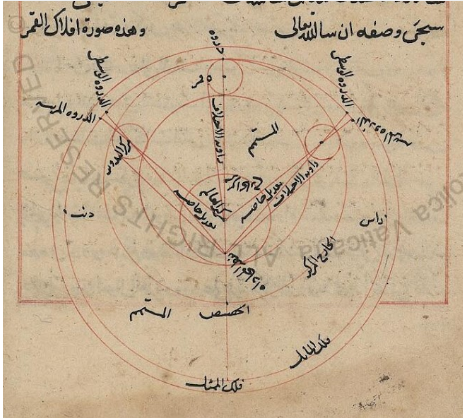
\includegraphics[width=5.5cm]{images/modele_lune_arabe.png}
		\end{subfigure}
		\hspace{1pt}
		\begin{subfigure}{0.30\linewidth}
			\centering
			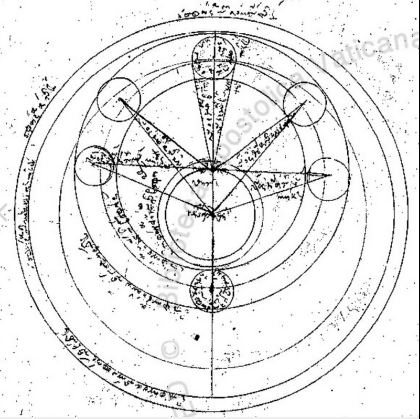
\includegraphics[width=5cm]{images/modele_lune_byz.png}
		\end{subfigure}
  		\hspace{1pt}
  		\begin{subfigure}{0.30\linewidth}
			\centering
			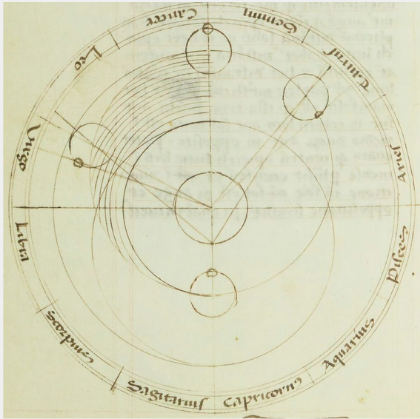
\includegraphics[width=5cm]{images/modele_lune_latin.png}
		\end{subfigure}
		\caption{Diagrammes astronomiques de tradition arabe, byzantine et latine}
		\label{fig:modeles_lune}
	\end{figure}

	\subsubsection{Bornes géographiques et chronologiques}
	Ayant la volonté de produire une étude des circulations et évolutions des diagrammes astronomiques, \eida s'attache à l'étude de sources provenant de sphères géographiques et temporelles larges : les pratiques eurasiatiques des sciences astronomiques partagent des éléments communs qui justifient une étude au cadre vaste, pour proposer une analyse transculturelle des continuités et divergences dans l'histoire de l'astronomie comme dans la culture visuelle. Pour répondre à cette volonté, le projet \eida s'appuie sur cinq corpus aux provenances temporelles et géographiques diverses, provenant de traditions diverses également, dans une volonté de représentativité. 
	
	Les manuscrits astronomiques arabo-persans, produits du \viii au \xviii siècle, représentent à eux seuls un corpus d'une grande diversité, aux traditions diverses aussi bien du point de vue des pratiques que de la provenance géographique. Les travaux produits dans ces contextes circulent à travers l'Eurasie du \ma au début de la période moderne, et influencent de nombreuses pratiques. Les manuscrits d'astronomie latins médiévaux sont produits majoritairement entre le \xiii et le \xvi siècle dans un contexte universitaire, et sont influencés par les traductions faites de l'arabe au latin de textes de tradition arabe ou persane. Les manuscrits byzantins, produits entre les \ix et \xv siècles sont à l'intersection des traditions helléniques, latines et arabo-persanes, et influencent considérablement les manuscrits astronomiques latins du \xv et du \xvi siècle. Les manuscrits sanskrits, dont la diversité reflète les nombreuses traditions établies sur près de deux millénaires, témoignent à partir du \xie siècle d'influences helléniques puis arabo-persanes. Les sources chinoises, dont le support n'est pas nécessairement le manuscrit, prennent souvent la forme d'imprimés par blocs xylographiques dont les matrices sont réemployées à travers plusieurs témoins. Ces documents témoignent des influences arabo-persanes puis latines des pratiques astronomiques chinoises à partir de la dynastie Ming\footnote{La dynastie Ming règne sur la Chine de 1368 à 1644.}. Les sources étudiées dans le cadre d'\eida proviennent essentiellement des dynasties Ming et Qing\footnote{La dynastie Qing, dernière dynastie impériale chinoise, règne de 1644 à 1912.}.
	
	Les bornes de ces cinq corpus représentent les bornes chronologiques et géographiques du projet. S'étendant du \viii au \xviii siècle, les périodes et aides étudiées se veulent représentatives du contexte afro-eurasien de la circulation des idées et des images. Ces corpus représentent, dans chaque cas, plusieurs milliers de manuscrits. Plusieurs centaines de manuscrits sont numérisés pour chaque tradition représentée dans le projet, permettant ainsi la représentativité espérée dans le cadre du projet \eida. Ces numérisations, mises à disposition par les institutions patrimoniales qui conservent ces témoins, représentent les sources primaires du projet, sur lesquelles seront appliquées les traitements en prévision de l'analyse par les chercheurs.

			\\
		
		\eida est un projet aux bornes chronologiques, géographiques et thématiques vastes, pour permettre une étude sur un temps long et dans un contexte global de la circulation des diagrammes astronomiques et des théories scientifiques qui les accompagnent. Dans cette démarche, proposer une étude quantitative, traitant un grand nombre de sources, permet de mettre en avant des motifs, connexions et évolutions en accord avec la diffusion afro-eurasienne des idées développées par Ptolémée. Les bornes définies dans cette partie permettent de délimiter un corpus d'images -- numérisations d'ouvrages manuscrits ou imprimés -- qui en tant d'objets numériques présentent également leurs propres problématiques.
        \clearemptydoublepage
        
        \chapter{Images et interopérabilité}
        Les sources étudiées dans ce mémoire sont des sources iconographiques, qui nécessitent des formats, ressources et méthodes pour le traitement des images en ligne, de la production de la ressource à sa publication. Les images digitales présentent des enjeux spécifiques, du point de vue de la technique, du droit et de la disponibilité. La mise en ligne et la diffusion d'une image fait suite à une longue chaîne de traitement qui a pour point de départ un objet matériel, et soulève des questionnements divers liés aux droits d'auteur, aux métadonnées, à la publication. Les spécifications \iiif tentent de répondre à un certain nombre de problématiques liées à la présence en ligne de ressources iconographiques, notamment du point de vue de l'interopérabilité et de l'ouverture des données : cette partie vise donc à présenter les solutions, possibilités et limites offertes par ce standard.
        
            \section{L’image comme source}
                % L'image comme source

\subsection{Construire un corpus d’images : enjeux et méthodes}
    \subsubsection{La numérisation, enjeu patrimonial}
	L'application à un corpus de sources historiques de méthodes numériques repose sur une première étape cruciale dans le traitement de ces sources : la numérisation des collections patrimoniales. De la bibliothèque au musée, la numérisation du patrimoine culturel est un enjeu crucial depuis le début des années 1990\footcite{baujardNumerisationPatrimoineCulturel2017}. Pensée initialement comme un outil de préservation, de valorisation et d'accessibilité aux collections\footcite{richardProgrammeNumerisationBibliotheque1993}, la mise à disposition des collections au format numérique ouvre également la voie à de nouvelles méthodologies de la recherche, notamment dans le champs disciplinaire des humanités numériques : dans le cadre d'un projet tel qu'\eida, qui prévoit des traitements automatiques des sources par des algorithmes de vision par ordinateur, la disponibilité des sources numérisées est un principe fondateur de la démarche de recherche. 
	
	La numérisation des données culturelles fait désormais partie des pratiques courantes des institutions culturelles, et plus particulièrement des bibliothèques, représentant une part intégrante du travail de conservation et de diffusion du patrimoine\footcite{claerrModeEmploi2017}. Dès le milieu 1990, des initiatives telles que Gallica\footcite{Gallica}, bibliothèque numérique de la \bnf, voient le jour, et mettent à disposition du public, au format numérique, les collections de la bibliothèque. Dans les années qui suivent, des initiatives telles qu'Europeana\footcite{Europeana} permettent le déploiement de projets de plus large envergure\footcite{claerrModeEmploi2017}, portant toujours cette responsabilité de préservation, diffusion et valorisation des collections dans un contexte international. La notion de patrimoine culturel numérique prend tout son sens, et Internet devient un espace permettant à des utilisateurs aux profils variés d'exploiter ces ressources numériques, et d'accéder à un patrimoine vaste, au-delà des limites physiques de la consultation des documents. Cependant, malgré les initiatives de soutien à la numérisation portées par les collectivités, ou même par l'État\footcite{claerrModeEmploi2017}, il est nécessaire de souligner les disparités, aussi bien sur le plan national qu'international, de ces entreprises de numérisation, souvent coûteuses : ainsi, il n'existe pas de réelle égalité entre les institutions dans la numérisation et la mise en ligne des collections, notamment du point de vue des financements, de la qualité des données produites et du volume de documents traités. Il s'agit d'un biais qu'il est nécessaire de prendre en compte, et particulièrement dans des projets de recherche appuyés sur des sources aux bornes géographiques internationales. 
	
	Dans le cas des corpus étudiés par le projet \eida, on compte, pour des sources qui représentent plusieurs centaines de milliers de documents, une somme de plusieurs centaines de documents numérisés, mis à disposition par les institutions patrimoniales européennes, chinoises et indiennes : nous constatons ainsi que les documents numérisés ne représentent qu'un fragment de la réalité des sources existantes, cependant, ces centaines de documents numérisés sont à la fois suffisantes et suffisamment représentatives pour le bon déroulé du projet.
	
	Les collections patrimoniales des musées présentent un tout autre enjeu en termes de mise en ligne : les œuvres conservées, allant bien au-delà du format livre, ont une diversité qui redéfinit entièrement le processus de numérisation\footnote{Par numérisation, dans le contexte muséal, nous entendons essentiellement la prise de photographies de haute qualité des œuvres d'arts.}. Tout comme les bibliothèques, les institutions muséales font face, avec le développement des pratiques numériques, à une transformation des pratiques de conservation pour inclure ces méthodes. Outre les aspects documentaires de la numérisation, le Web est un lieu d'exposition à part entière, et la numérisation des œuvres présente ainsi un intérêt stratégique en termes de valorisation et de visibilité\footcite{baujardNumerisationPatrimoineCulturel2017}. Dans le monde muséal, néanmoins, l'accès libre aux images n'est pas aussi systématique qu'en bibliothèque\footnote{Pour comparaison, Gallica représente aujourd'hui près de 10 millions de documents, et la base de la \acrfull{rmn} compte 600 000 œuvres numérisées.} : il existe bel et bien des projets de numérisation de grande envergure, tels que Google Arts \& Culture\footcite{GoogleArtsCulture}, publié en 2011. La vocation de ce type de projets, cependant, semble plutôt être la création d'espaces d'exposition dématérialisés permettant de mettre en valeur les œuvres pour des spectateurs, plutôt que la véritable mise à disposition de ces images pour un usage par des utilisateurs. Nous soulignons, notamment, dans le cas de Google Arts \& Culture, l'impossibilité de copier les images avec un clic droit, et l'absence de bouton pour le téléchargement des numérisations sur un certain nombre de pages : les numérisations sont faites pour être vues, et non utilisées\footnote{Certaines œuvres du projet sont disponibles sur Wikimedia, mais ces images en accès libre ne représentent qu'un fragment des œuvres numérisées dans le cadre du projet. De plus, les musées français sont très peu représentés dans cette sélection. \cite{CategoryGoogleArt}}. 
	
	Une étude menée entre 2019 et 2020 par le Musée National de Tokyo souligne, en parallèle, les disparités dans la qualité des numérisations, qui ne permet ainsi pas de considérer qu'un objet numérisé ou photographié l'est nécessairement dans une qualité exploitable\footcite{sakaiDigitizingDisparityMuseum2021}, notamment parce que les besoins en termes de qualité ne sont pas les mêmes pour des œuvres en 2D et des œuvres en 3D, qui souffrent particulièrement de la mauvaise qualité des numérisations. Ainsi, en prenant en compte ces critères, il est nécessaire de soulever la question de la réelle exploitabilité des images mises en ligne, et particulièrement dans le cadre de projets en vision artificielle qui reposent, dans leurs fondations, sur la disponibilité et la qualité des images du corpus choisi. Des initiatives récentes tentent cependant de pallier à ces lacunes des institutions patrimoniales quant à la mise à dispostion des images, comme la création en 2015 d'une \api donnant accès aux reproductions de la base photographie de la \acrshort{rmn}\footcite{APIRMNGrandPalais}, mais la norme, pour ces images d'œuvres d'art, reste loin de l'\textit{open access}\footcite{mancaNouveauxDefisAgences2018}. 

    \subsubsection{Droit d'auteur et coût des images}
	La numérisation et la mise en ligne de documents patrimoniaux implique également de prendre en compte la question des droits d'auteur, qui régit souvent les possiblités des institutions en termes de libre accès, et impacte par conséquent les projets, aussi bien du point de vue des exploitations possibles que de la publication de leurs résultats\footcite{jacquotDecrireTranscrireDiffuser2017}. 
	
	Une œuvres originale est protégée au titre du droit d'auteur : ce droit comprend le droit moral, perpétuel et inaliénable, qui donne droit au respect de l'œuvre et du nom de son auteur, ainsi que le droit patrimonial, qui donne à l'auteur et ses ayants droit le droit d'autoriser ou non la reproduction et la diffusion de l'œuvre\footcite{sepetjanRespecterDroitPropriete2017}. Les droits patrimoniaux s'éteignent soixante-dix ans après la mort de l'auteur, et l'œuvre entre alors dans le domaine public\footnote{Il existe des cas particuliers, notamment pour les œuvres collectives ou les journaux, ainsi que pour les publications posthumes. \cite{GuidePratiquePour}.}. Il n'existe pas d'exception au droit d'auteur pour une numérisation mise en ligne sur Internet\footcite{sepetjanRespecterDroitPropriete2017}. Ces droits, qui s'appliquent à l'œuvre originale, ne sont pas nécessairement ceux qui nous intéressent dans le cadre d'un projet de recherche en histoire, dont les œuvres du corpus ont souvent rejoint le domaine public. La photographie d'une œuvre, cependant, peut faire l'objet du droit d'auteur, si celle-ci n'est pas considérée comme une reproduction servile\footnote{Pour que la photographie d'une œuvre d'art ne soit considérée une reproduction servile, il est nécessaire que celle-ci témoigne d'une intervention artistique de la part du photographe. Un choix de composition, de lumière ou un traitement avec un logiciel peuvent être considérés comme des interventions artistiques.}.
	
	Outre le droit d'auteur et les droits du photographe, les institutions peuvent exiger une redevance de réutilisation ou de prestation d'un service pour l'utilisation de leurs images, qui sert à couvrir, par exemple, les frais engagés pour la production du cliché, le traitement de la demande, ou la recherche iconographique\footcite{GuidePratiquePour}. Beaucoup d'institution, telles que la \bnf et l'\inha\footcite{denoyelleProposCoutImages2021}, proposent des tarifications particulières pour des projets académiques, scientifiques ou non commerciaux, et n'appliquent un coût qu'en cas de demande de numérisation d'œuvres qui ne sont pas déjà numérisées. Les projets de recherche peuvent ainsi faire le choix de construire leurs corpus en prenant en compte les documents déjà disponibles, et mis en ligne sous licence libre\footnote{Pour permettre aux chercheurs de traiter leurs numérisations sous droits avec les outils de la plateforme \eida, il a été décidé de proposer une option -- sous la forme d'un champs à cocher dans le formulaire de saisie -- pour que la numérisation envoyée ne soit pas rendue publique.}.

\subsection{Images et données ouvertes}
    \subsubsection{Licences Creative Commons}
	Pour favoriser la libre circulation des images sur le Web, des licences ont été créées pour encadrer la réutilisation des numérisations. Dès 2001, les licences Creative Commons\footnote{Ces licences ne sont plus reconnues par l'État français depuis 2016. \cite{denoyelleSavoirLicenceEtalab2021}.} sont créées avec la vocation de favoriser la diffusion et le partage des images dans un contexte numérique, en assouplissant notamment les droits de propriété intellectuelle pour s'adapter à ce nouveau cadre. Ces licences se basent sur un système de quatre options qu'il est possible de combiner pour créer six licences différentes. Ces options sont attribution (BY), non commercial (NC), sans modification (ND) et partage à l’identique (SD)\footcite{GuidePratiquePour}. 
	
	À partir de 2011, l'État français créée ses propres licences ouvertes, comme la licence unique Etalab, qui vise à \og permettre et encourager la réutilisation des données publiques\footcite{denoyelleSavoirLicenceEtalab2021} \fg. Une deuxième version, publiée en 2017, se veut compatible avec la licence CC BY, c'est-à-dire une licence ouverte avec attribution de l'œuvre à son auteur.
	
	Les données ouvertes sont un enjeu central des politiques culturelles : dans un contexte patrimonial, ces licences libres, conçues pour adapter les droits de propriété intellectuelle au contexte particulier du numérique, permettent ainsi la circulation, la diffusion et le partage de l'information. Il n'existe pas encore de cadre juridique international régissant l'utilisation des images produites par numérisation de collections patrimoniales, ainsi, les institutions sont soumises au droit spécifique du pays qui les abrite. En l'absence d'un encadrement global des pratiques, les utilisateurs -- et notamment la communauté de la recherche -- font face aux exceptions propres à chaque contexte national, qui représentent encore un obstacle. Une réflexion autour de ce cadre juridique international permettrait, en parallèle, d'harmoniser à une échelle globale les formats des données ouvertes\footcite{benhamouDroitAuteurMusees2016}, pour en faciliter la réutilisation par les institutions et par les projets.

    \subsubsection{Enjeux techniques : images et métadonnées}
	Le document numérique obtenu à la suite d'une processus de numérisation est, en réalité, constitué de plusieurs fichiers répondant à des besoins différents pour la mise en ligne. Chacun de ces éléments représente ses propres enjeux techniques, dont la gestion impacte la qualité et l'exploitabilité des images mises en ligne à la suite d'entreprises de numérisation.
	
	Les fichiers images issus d'un processus de numérisation peuvent avoir plusieurs formats\footnote{Un format décrit la manière dont les informations sont organisées dans un fichier.} aux propriétés similaires mais différentes. En premier lieu, il est de bonne pratique de privilégier un format ouvert\footcite{besseNumerisationMasseVers2019}, par opposition à un format propriétaire qui nécessite un logiciel spécifique pour être lu. Le choix d'un format ouvert permet d'assurer l'accessibilité des données produites. Les formats \acrfull{tiff} et \acrfull{jpeg} sont favorisés dans le contexte de numérisation des collections patrimoniales, parce qu'ils permettent notamment la compression des fichiers\footnote{La compression sans perte s'effectue par identification et suppression des redondances, c'est-à-dire des pixels identiques. Cette méthode n'est pas irréversible, il est possible de décompresser le fichier.} tout en maintenant la haute qualité des images\footcite{DigitalImages2020}. Les choix effectués par les institutions impactent la qualité des numérisations produites qui, sur un plus long terme, impacte aussi bien la préservation des données, l'expérience des utilisateurs qui consultent les images, et l'exploitabilité des fichiers par des projets. La question de la qualité des images est cruciale dans le cadre d'un projet de recherche en vision artificielle, puisque celle-ci a la possiblité d'impacter les performances de l'algorithme utilisé, et d'affecter négativement les interprétations du modèle\footcite{bergstromImageQualityComputer2023}.
	
	Les fichiers images sont systématiquement accompagnés de métadonnées de diverses catégories, qui visent à décrire et identifier le document. Bien qu'il n'existe pas de standard international obligatoire concernant les métadonnées de numérisation, la standardisation des fichiers de métadonnées selon certains standards spécifiques permet de fluidifier la communication et les échanges entre institutions, dans une perspective interopérable qui permettrait de sortir des silos de données\footnote{Un silo de données est un ensemble de données isolées ou difficilement accessibles. Dans le contexte des institutions patrimoniales et des établissements de recherche, dont les données se veulent publiques et partagées, les silos de données sont un obstacle à la mutualisation et à l'échange des ressources et informations.}. Les métadonnées sont de plusieurs types : descriptives\footnote{Pour identifier le contenu du document numérique, le rattacher au document original.}, administratives\footnote{Pour gérer les droits d'accès, préserver les informations techniques, suivre les modifications du fichier et garantir son intégrité.}, structurelles\footnote{Pour rattacher les fichiers entre eux et reconstituer la structure du document.} ; elles ont pour vocation de gérer tous ces aspects du document numérique. Ces métadonnées sont cruciales pour l'identification et la classification des documents numérisés, mais aussi pour permettre la recherche et la navigation à travers les collections. Malgré leur importance, les différentes institutions ont une gestion profondément hétérogène de leurs métadonnées, sans uniformisation nationale ou internationale, et avec une disparité profonde entre les différents types d'institutions patrimoniales.
	
	Pour pallier à cette disparité dans la gestion des métadonnées et au manque de standards pour le partage des images en ligne, des initiatives internationales ont vu le jour, visant à mettre fin à cette gestion en silo des données des institutions patrimoniales pour faciliter les échanges et la mise à disposition des données dans une optique de libre accès.
        
            \section{\label{stardardIiif}Le standard IIIF}
                % Le standard IIIF

\subsection{IIIF et les données ouvertes}
    \subsubsection{Principes et objectifs}
	Le standard \iiif\footcite{IIIFInternationalImage} est une initiative collaborative lancée en 2011 par un groupement d'institutions\footnote{Les collaborateurs à l'initiative du projet sont la British Library, la \bnf, Stanford University, les Bodleian Libraries, la Bibliothèque nationale de Norvège, la Bibliothèque nationale de Los Alamos et Cornell University.} attachées à faciliter la diffusion sur le Web des ressources iconographiques des collections patrimoniales \footcite{cramerInternationalImageInteroperability2011}. La volonté de développement de ce standard provient du constat que, malgré la nécessité d'un accès global aux images numériques pour la transmission du patrimoine culturel, un grand nombre de ces ressources restent, sur Internet, isolées dans des silos d'informations dont l'accès n'est possible que par des applications spécifiques à chaque institution\footcite{cramerInternationalImageInteroperability2011}, rendant complexe le partage et la mise en commun des ressources.
	
	De cette observation est née la volonté de créer un outil proposant des méthodes standardisées de partage sur le Web des images et de leurs métadonnées, pour toute institution qui souhaiterait partager numériquement ses collections. \iiif propose ainsi un standard dont les fonctionnalités vont au-delà de celles d'un navigateur, capable d'afficher des formats libres d'image\footnote{\iiif propose également, depuis 2020, un service dédié aux fichiers vidéo, que nous n'abordons pas dans ce mémoire car les projets étudiés portent tous sur des images fixes.}, sans proposer plus d'interaction avec les images servies\footcite{HowItWorks}. \iiif propose ainsi des outils interopérables, libres d'accès, permettant notamment de zoomer en profondeur sur les images, d'y appliquer des traitements visuels simples, de reconstruire la structure du document ou de les annoter.
	
	Pour assurer ces fonctionnalités, \iiif s'appuie sur deux \api\footnote{Une \api est une interface logicielle permettant de connecter entre eux des logiciels pour échanger des données, des fonctionnalités ou des services.} : l'\api Image et l'\api Présentation. Ces \api sont le socle du standard, elles en assurent la cohérence afin que les images puissent être partagées de manière fluide entre les institutions et projets. Le cœur du standard \iiif, qui fait tout son intérêt dans le contexte décrit précédemment du partage des images sur le Web, est en effet l'interopérabilité : \iiif assure ainsi la portabilité entre les visualiseurs, pour permettre une transmission réellement fluide de l'information.
    
    \subsubsection{Les API IIIF}
	Le fonctionnement du standard \iiif s'appuie sur deux éléments essentiels : l'envoi des images depuis les serveurs, et leur visualisation. 
	
	L'\api Image définit les spécifications pour un service renvoyant une image en réponse à une requête \http ou \https : à partir d'une \uri valide, l'image peut être affichée dans un visualiseur, ou dans un navigateur. L'\uri peut spécifier, dans sa requête, la région, la taille, la rotation, la qualité ou le format de l'image demandée, suivant des instructions spécifiques prédéfinies par le standard\footcite{ImageAPI}. En ajustant les paramètres, l'utilisateur peut ainsi obtenir une image qu'il peut modifier en accord avec ses besoins sans passer par un éditeur spécifique. L'\api Image, développée pour des clients tels que les applications d'institutions patrimoniales, peut être implémentée sans l'\api Présentation : seule, elle permet notamment un zoom rapide et profond sur des images en très haute résolution.
	
	L'\api Présentation permet d'introduire des fonctionnalités plus vastes en termes d'informations liées aux images : par le biais d'un manifeste au format \json, elle attache aux images des métadonnées descriptives, administratives et structurelles qui définissent la manière dont elles seront présentées dans un visualiseur. Le manifeste permet notamment de rassembler en un fichier les différents éléments d'un objet \iiif\footcite{HowItWorks}, et notamment les séries d'images\footnote{Cette fonctionnalité est particulièrement intéressante pour les numérisations d'ouvrages, puisqu'elle permet de regrouper en un fichier toutes les pages numérisées.}, tout en gérant également leur ordre dans le document numérique. Le manifeste contient généralement des informations d'identification de l'objet original\footnote{On retrouve notamment le titre, l'auteur, l'institution de conservation, le numéro d'inventaire ou la cote, et les informations sur les droits de diffusion.}, et peut être enrichi d'annotations sur l'objet ou son contenu\footcite{PresentationAPI}.
	
	Pour afficher les images et les informations liées, il existe une multitude de visualiseurs\footcite{IIIFViewers} aux fonctionnalités différentes, tous compatibles avec tous les manifestes \iiif, quelle que soit leur institution d'origine. Ainsi, les ressources produites par les institutions peuvent être consultées par le biais d'outils libres, accessibles à tous. Pour aller au-delà des fonctionnalités proposées par les deux \api centrales du standard, quatre autres \api ont été développées, pour gérer d'autres besoins liés à mise à disposition d'images tout en respectant des principes standardisés\footcite{HowItWorks}.
    
    \subsubsection{Anatomie d'un manifeste}
	Pour constituer les éléments retournés par les \api \iiif, il existe un modèle de données spécifique, qui assure la caractérisation des objets selon des normes communes, qui permettent de conserver l'interopérabilité du standard. Il existe ainsi des types de ressources, ou classes, précisément définies, avec une hiérarchie fixe (fig. \ref{fig:iiif_data_model}), qui permettent de décrire les objets numérisés au format \json.
	
	Un manifeste est un fichier au format \json. Du point de vue de la donnée, la classe \textit{Manifest} permet de décrire un objet composé, une œuvre dans sa totalité : elle contient ainsi un ensemble de métadonnées descriptives la concernant (titre, auteur, institution de conservation, licence), et permet, si nécessaire, de reconstituer la structure de l'objet à partir des \textit{Canvases}.
	
	Le \textit{Canvas} est un conteneur de niveau inférieur au \textit{Manifest}, qui permet de représenter une vue spécifique d'un objet, et les métadonnées qui y sont associées. Si nécessaire, un élément de niveau supérieur peut exister entre les \textit{Canvases} et le \textit{Manifest} : il s'agit des \textit{Ranges}, qui permettent de décrire une séquence de \textit{Canvases}.
	
	Il existe, à un niveau supérieur au \textit{Manifest}, une classe \textit{Collection}, qui assure une plus grande flexibilité du modèle pour les projets qui souhaiteraient réunir plusieurs objets dans une catégorie plus large. Une \textit{Collection} peut représenter une liste de \textit{Manifests}, ou une liste de \textit{Collections}, permettant ainsi de regrouper des objets ou groupes d'objets selon un cadre défini, qui facilite la navigation dans un ensemble restreint de ressources liées\footcite{PresentationAPI}.
	
	Pour un manifeste ne contenant que des images et leurs métadonnées, ces éléments suffisent à construire un fichier cohérent et fonctionnel, qui pourra être lu par un visualiseur \iiif.
	
	Pour annoter les images d'un manifeste, il existe une série de types de ressource additionnels qui contiennent les annotations selon une hiérarchie précise, et les rattache à un \textit{Canvas} spécifique. L'\textit{Annotation Page} contient une liste ordonnée d'\textit{Annotations} pour un \textit{Canvas} : pour annoter un manifeste, il existe donc autant d'\textit{Annotation Pages} qu'il existe de \textit{Canvases} annotés.
	
	La classe \textit{Annotation} fait le lien entre le contenu de l'annotation (\textit{Content}) et le \textit{Canvas}\footcite{PresentationAPI} : ce type de ressource permet d'assurer l'interopérabilité du modèle, puisqu'elle permet l'alignement des annotations et des images, y compris dans le contexte d'annotations produites par un utilisateur différent du créateur du manifeste. Ainsi, ce modèle de données permet la collaboration entre plusieurs utilisateurs à partir d'un manifeste produit par une institutions, et rend possible la réutilisation des images comme des manifestes dans des projets ultérieurs, avec la fluidité d'un modèle partagé, standard, qui ne nécessite aucun effort d'alignement entre institutions.
	
	\begin{figure}[h]
		\centering
		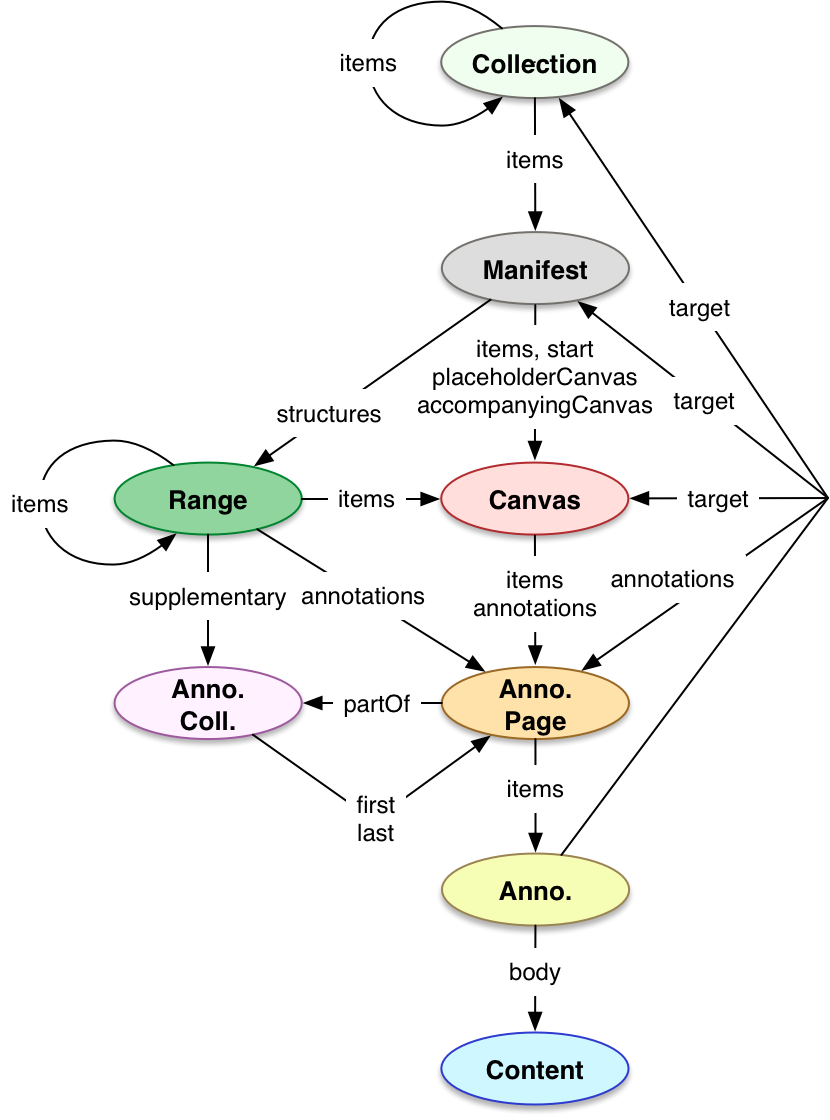
\includegraphics[width=10cm]{images/modele_donnees_iiif.png}
		\caption{Modèle de données \iiif pour la description d'un objet}
		\label{fig:iiif_data_model}
	\end{figure}
    
\subsection{IIIF, un modèle universel ?}
    \subsubsection{Limites de l'interopérabilité du standard}
	\iiif est ainsi pensé comme un standard universel permettant aux institutions et aux projets qui le souhaitent de partager leurs ressources, de les mettre à disposition en assurant la possibilité de leur réutilisation : dans une optique de science ouverte, \iiif permet de partager aisément les résultats de projets de recherche impliquant des images.
	
	Cependant, malgré l'existence d'un modèle de données standard pour la description des objets, \iiif présente des limites dans son universalité. En effet, malgré son cadre construit pour assurer l'interopérabilité des manifestes, le modèle n'est en pratique pas employé de la même manière par toutes les institutions, et nécessite donc une adaptation des développements faits autour de \iiif pour prendre en compte ces exceptions. Nous constatons, par exemple, que si les ressources images sont supposées être intégrées au manifeste dans un conteneur \textit{Canvas}, certaines institutions -- comme la bibliothèque univeristaire de Yale -- utilisent plutôt des \textit{Items} (fig. \ref{fig:manifests_canvas}), modifiant ainsi profondément la structure du manifeste \iiif tout en conservant un fichier lisible par les visualiseurs. L'application du standard varie ainsi d'une institution à l'autre, sans altérer le fonctionnement des outils de base de \iiif, mais en provoquant cependant une déperdition de son universalité pour des projets qui souhaiteraient développer des outils autour de ces manifestes. 
	
	Dans un projet reposant sur l'exploitation d'images d'objets patrimoniaux, tels que les projets décrits dans ce mémoire, il est ainsi nécessaire de prendre en compte ces exceptions techniques : dans le cadre du projet \eida, la récupération des images est effectuée par un algorithme spécifique\footcite{albouyIiifdownloader2023}, qui parse un manifeste \iiif déposé par un utilisateur dans l'application du projet et en extrait des fichiers images pour les enregistrer. Dans le développement de cet algorithme, il a ainsi été nécessaire de prendre en compte les exceptions possibles, pour ne pas créer d'erreur en cas de dépôt d'un manifeste à la structure différente.

	\begin{figure}[h]
		\begin{subfigure}{1\linewidth}
			\centering
			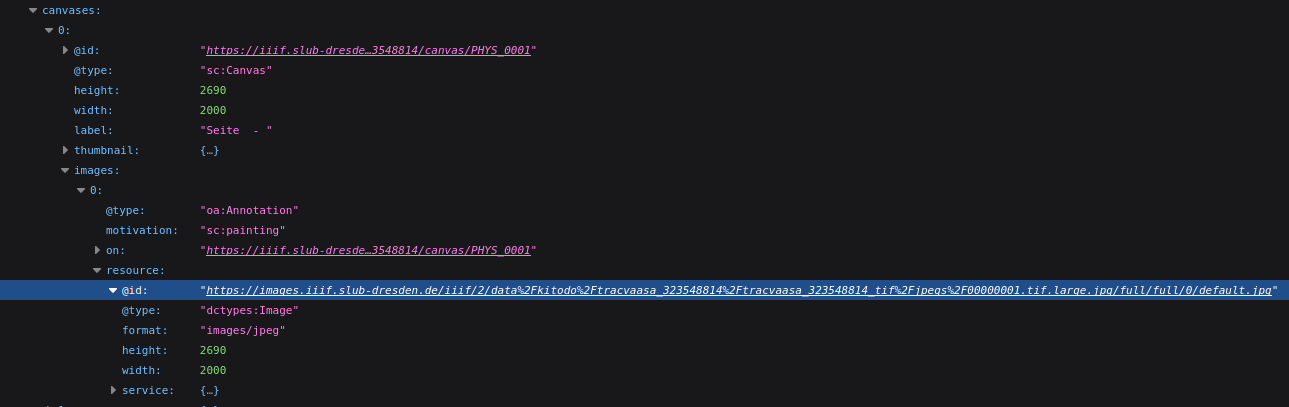
\includegraphics[width=15cm]{images/dresden_manifest.png}
			\subcaption{Manifeste \iiif de la bibliothèque universitaire de Dresde avec \textit{Canvases}}
		\end{subfigure}
		\hspace{1pt}
		\begin{subfigure}{1\linewidth}
			\centering
			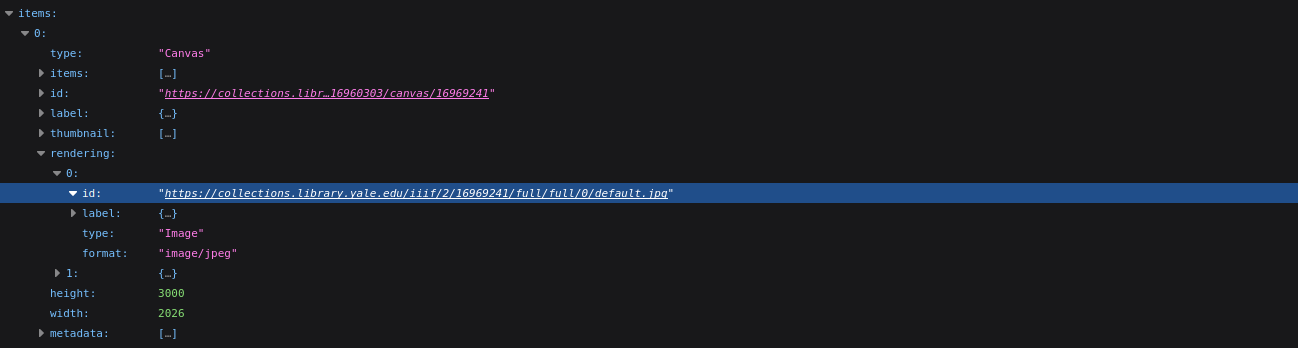
\includegraphics[width=15cm]{images/yale_manifest.png}
			\subcaption{Manifeste \iiif de la bibliothèque universitaire de Yale avec \textit{Items}}
		\end{subfigure}
		\hspace{1pt}
		\caption{Comparatif des ressources contenant les images de deux manifestes \iiif}
		\label{fig:manifests_canvas}
	\end{figure}

    \subsubsection{Implémentation de IIIF : un réflexe global ?}
	Pour les projets de recherche exploitant des images respectant le standard \iiif, il se pose la question des institutions ayant fait le choix de gérer leurs images différemment. En effet, si de nombreuses institutions ont adopté le standard et mis en ligne des centaines de millions d'images compatibles depuis la naissance de l'initiative\footcite{malloryIIIFMuseumsExplained2019}, il n'est ni obligatoire ni systématique, et il reste ainsi un nombre certain d'établissements qui gèrent leurs images avec des outils techniques différents, et restent ainsi exclus du standard. Les musées, notamment, et particulièrement les musées hors Amérique du Nord, exploitent encore peu les possibilités offertes par \iiif en termes de partage des images\footcite{IIIFMuseumsFrance2023}, et restent en marge de cette initiative de facilitation de la mise en commun et de l'exploitation des ressources iconographiques.
	
	Il n'est cependant pas envisageable, dans le cadre d'un projet de recherche, d'exclure totalement les sources provenant d'institutions n'utilisant pas le standard \iiif : il est donc nécessaire, dans le développement d'outils numériques pour la gestion des images, de prendre en compte ces sources aux formats différents, qu'il faut traiter pour les rendre exploitable de la même manière que le sont les images extraites de manifestes \iiif. Ainsi, dans la chaîne de traitement des images, une réflexion doit être menée pour l'intégration d'autres formats, tels que les PDF pour les numérisations d'ouvrages, ou les fichiers images indépendants. Malgré la fluidité du traitement des sources permise par l'existence d'un standard, il est ainsi nécessaire de réfléchir à des solutions techniques au-delà des limites de ce dernier, pour ne pas exclure des corpus les sources numérisées présentant un intérêt pour la recherche. 
	
	Dans un projet de recherche en vision artificielle, l'utilisation du standard \iiif permet, d'une part, la constitution aisée d'un corpus d'images, qu'il est possible de récupérer directement sur les sites des institutions à l'aide des \api : le standard \iiif fluidifie fortement les échanges et la réutilisation des documents numérisés, et permet de construire un outil générique pour le traitement de sources numériques provenant d'institutions diverses. Il reste cependant de nombreux cas où une chaîne de traitement parallèle doit être développée, pour pallier à l'absence d'implémentation du standard dans certaines institutions. D'autre part, l'utilisation du standard \iiif pour la publication en ligne des données du projet permet également d'envisager leur réutilisation future par d'autres initiatives, en s'assurant de l'interopérabilité des résultats produits, dans une démarche de science ouverte.

        	\\
        
        Les sources iconographiques sont soumises à un ensemble de restrictions, du point de vue du format, des métadonnées ou des droits, qui manquent encore d'une uniformité internationale et entre institutions qui rendrait fluide le partage de ces ressources sur Internet et entre les projets de recherche. Dans un projet impliquant l'utilisation d'algorithmes de vision artificielle, qui repose alors sur le traitement d'un volume important d'image, la mise en ligne de ces documents est un enjeu crucial, sur lequel repose d'une part la possibilité de constituer un corpus exploitable, ainsi que la publication des résultats du projet, qui peuvent également prendre la forme d'images numériques. Dans une optique de science ouverte, l'utilisation de standards et d'outils tels que ceux développés par le consortium \iiif permet d'assurer le partage d'images et de données respectant les mêmes formats, exploitables avec des outils libres, et d'avancer vers une abolition des silos de données, qui faciliterait notamment la construction de corpus massifs pour l'apprentissage machine. 
        \clearemptydoublepage
        
        \chapter[Corpus historiques et jeux de données]{Corpus historiques et jeux de données pour l’apprentissage machine}
        La vision artificielle et l'apprentissage machine permettent le traitement de corpus d'images massifs par des méthodes quantitatives qui permettent aux historiens de traiter un volume de données bien plus important qu'une approche manuelle, ouvrant ainsi la voie à de nouvelles approches. Cette partie présente les bonnes pratiques à mettre en place afin d'assurer la pertinence de l'utilisation de ces outils, et d'en faire des traitements efficaces en accord avec les ambitions des projets.
    
            \section{Dimensions et cadre}
                % Dimensions et cadre

\subsection{La tentative de l’exhaustivité}
    \subsubsection{Représentativité et pertinence}
	L'approche computationnelle de corpus de sources historiques permet le traitement d'un volume d'images inenvisageable sans automatisation, qui redéfinit les méthodes de constitution d'un corpus pour prendre en compte cette quantité de données qu'il est possible de considérer à l'aide d'outils numériques\footcite{klinkeBigImageData2016}. L'apprentissage profond permet d'envisager une redéfinition des méthodes des historiens et historiens de l'art, en intégrant une part d'automatisation dans le traitement des sources iconographiques, permettant ainsi d'envisager l'exploration de corpus bien plus vastes\footcite{moiraghiExplorerCorpusImages2018} par des méthodes quantitatives\footcite{klinkeBigImageData2016}.
	
	Dans le cadre du projet \eida, ces possibilités ouvertes par l'intégration de techniques de vision artificielle dans le traitement du corpus permet ainsi d'envisager des bornes larges, définies précédemment, sur le plan géographique comme chronologique, tout en assurant un traitement d'un grand nombre de sources -- plusieurs centaines ou milliers d'images -- pour chaque contexte étudié. 
	
	Le projet \vhs s'appuie également grandement sur la vision artificielle appliquée à la recherche de similarité, dans le cadre d'une étude de la circulation des savoirs scientifiques par le biais de l'illustration : les corpus constitués pour le projet ont donc été pensés pour offrir un regard pertinent sur ces questions, et sélectionnés avec une volonté de représentativité géographique, chronologique et thématique\footcite{Corpus}. Leur analyse portera ainsi sur un ensemble de plus de 10 000 images d'animaux, de plantes et de minéraux.
	
	Ainsi, l'intégration aux projets d'humanités de méthodes de vision artificielle permet d'envisager l'étude de corpus larges, vastes, et de porter un regard sur des zones géographiques larges, sur des périodes étendues, avec la possibilité de traiter des corpus massifs par des approches quantitatives développées en collaboration avec les historiens.

    \subsubsection{Données d'entraînement}
	Au-delà de la pertinence du corpus pour un projet de recherche donné, il est nécessaire, pour l'entraînement d'un modèle de vision artificielle, de prévoir un fragment du corpus dédié à la constitution d'un ou de plusieurs jeux de données d'entraînement\footnote{Un jeu de données d'entraînement comptant en général plusieurs centaines d'exemples, il est possible, à cette étape, d'évaluer la pertinence véritable du développement d'un modèle dédié au traitement du corpus global du projet. \cite{strienComputerVisionHumanities2022}}. La représentativité est un élément clé de ces corpus restreints, qui doivent à leur échelle comporter suffisamment de cas d'études différents pour englober les situations rencontrées dans le corpus global, et ainsi produire un modèle apte à appréhender toutes les situations rencontrées dans un contexte d'inférence. Un dialogue entre les chercheurs et les ingénieurs est alors nécessaire, pour établir les besoins d'un point de vue technique comme d'un point de vue scientifique, afin d'obtenir en finalité un outil performant, apte à traiter le corpus du projet. Les chercheurs ayant une connaissance scientifique de la typologie des sources rencontrées dans le cadre du projet, ils sont ainsi à même d'estimer la diversité des images que rencontrera le modèle, et donc de construire un jeu de données d'entraînement représentatif et pertinent, en accord avec les bornes définies du projet.
	
	Le projet \eida, dont le cadre géographique s'étend de l'Europe à l'Asie, du \viii au \xviii siècle, est ainsi vaste en termes de sources historiques et de diagrammes représentés. Les jeux de données d'entraînement doivent être représentatifs d'un point de vue thématique, en proposant des diagrammes aux formats et apparences diverses, en accord avec les typologies variées retrouvées dans le corpus ; mais ceux-ci doivent aussi prendre en compte la diversité des supports. Le corpus d'\eida comporte en effet des sources manuscrites comme des sources imprimées, qu'il est donc nécessaire de traiter conjointement. Il a été envisagé, pour des questions de performance, de produire un modèle de vision entraîné spécifiquement sur des sources manuscrites, et un second modèle entraîné sur des sources imprimées, afin de dissocier totalement le traitement de ces deux supports dans l'application finale\footnote{L'entraînement des modèles de détection d'objet n'ayant pas encore été effectué, il est actuellement impossible de tirer des conclusions quant à la pertinence de ce choix.}. Dans un corpus aussi varié linguistiquement que celui du projet \eida, il est également crucial de sélectionner un jeu de données d'entraînement diversifié du point de vue des langues, pour s'assurer de l'efficacité du modèle sur des sources aux provenances diverses : nous constatons en effet que les premières détections faites avec des modèles de détection pré-entraînés\footnote{Nous traitons de ces modèles dans la partie II.1.2.} sont satisfaisantes sur des sources latines ou grecques, mais qu'ils performent peu efficacement sur des sources chinoises, où chaque idéogramme est détecté comme une image.
	
	Ainsi, l'automatisation d'une partie de la chaîne de traitement des sources permet de construire un corpus de recherche vaste en offrant l'opportunité d'analyser un volume massif de sources historiques : ces possibilités sont particulièrement intéressantes dans le cadre de projets de recherche inscrits dans l'histoire de la circulation des idées, des images et des théories, puisque les corpus construits peuvent être représentatifs de multiples cadres géographiques, temporels et thématiques, sans craindre un surplus de sources à traiter. Pour construire des outils pertinents pour le traitement de ces corpus massifs, il est cependant nécessaire d'avoir un regard global sur leur contenu, pour reproduire à moindre échelle leur représentativité dans des jeux de données d'entraînement, nécessaires au développement de modèles de vision artificielle pertinents pour des sources étudiées.
    
\subsection{Automatiser le traitement de corpus massifs}
    \subsubsection{Possibilités de la \cv}
	La vision artificielle offre, pour le traitement de ces larges corpus, la possibilité d'automatiser certaines étapes spécifiques qui interviennent en parallèle d'étapes d'analyse par les chercheurs. Il n'existe ainsi pas de chaîne de traitement\footnote{Nous employons également le terme de \textit{workflow}.} totalement automatisée, où l'historien n'interviendrait pas dans le traitement des sources étudiées. En effet, l'intégration de la vision artificielle aux méthodes des historiens n'existe que conjointement à des interventions humaines, qui assurent la pertinence des traitements effectués et apportent une analyse nécessaire.
	
	L'une des premières applications de la vision par ordinateur exploitée dans les projets étudiés est la détection d'objet dans les images : pour le traitement de sources numérisées, la détection d'objet présente des applications diverses. Il s'agit, le plus souvent, de la première étape d'une chaîne de traitement ; permettant, par exemple, dans l'étude de sources manuscrites ou imprimées contenant du texte et des illustrations, d'extraire les images présentes dans ces sources\footcite{buttnerCorDeepSacroboscoDataset2022}. Dans les projets \eida et \vhs, cette étape de détection des images dans les ouvrages est faite dans une optique de segmentation des pages, pour en extraire les illustrations qui seront ensuite traitées par d'autres algorithmes de vision, tels que des algorithmes de recherche de similarité ou de vectorisation. D'autres projets, cependant, proposent dès l'étape de détection une classification des illustrations par typologie, pour permettre une première analyse et un premier regard sur la place de ces objets détectés dans les sources étudiées : l'application CorDeep\footcite{CorDeep}, développée par le Max Planck Institute for the History of Science en partenariat avec BIFOLD pour l'extraction d'éléments visuels dans les sources historiques, propose de classifier les illustrations détectées en quatre catégories\footnote{\textit{Content Illustrations}, \textit{Initials}, \textit{Decorations} et \textit{Printer's Marks}.}, appliquant dès la détection un premier traitement pour l'analyse des illustrations par les chercheurs, qui peuvent ainsi plus aisément naviguer des corpus de numérisations d'ouvrages par le biais des images.
	
	La recherche de similarité compte parmi les applications les plus directes du \dl\footcite{moiraghiExplorerCorpusImages2018} : il est possible, à l'aide d'un modèle entraîné sur un jeu de données restreint, d'effectuer sans supervision des comparaisons entre toutes les images du corpus, pour les réunir en séries ou groupes qui seront ensuite analysés par les historiens. Le développement d'un tel outil exemplifie les possibilités offertes par l'intelligence artificielle pour la navigation de gros corpus : elle permet de classifier les images en vue de leur étude en constituant des séries iconographiques aux caractéristiques visuelles similaires, selon un score de similarité calculé par l'algorithme. Dans le cas d'une étude des circulations des illustrations scientifiques, la constitution de ces séries permet aux chercheurs d'effectuer une analyse sur l'évolution des théories scientifiques, par le regroupement d'images de traditions différentes présentant des éléments similaires. L'automatisation de cette étape permet ainsi de tracer des parallèles entre un grand nombre d'images, en lançant la détection sur des corpus très larges qu'il serait difficile de traiter manuellement.
	
	La \cv permet également d'envisager des traitements pour l'édition, et particulièrement dans le cas d'objets scientifiques tels que les diagrammes, dont la mise en forme est un questionnement à part entière pour l'édition des textes qu'ils illustrent. La détection de contours (ou \textit{edge detection}) est une étape fondamentale pour le traitement des images en vision artificielle : combinée à des méthodes de détection des lignes\footcite{linComprehensiveReviewImage2023}, il devient envisageable d'automatiser la transformation d'images au format .tiff ou .jpeg en objets plus aisément manipulables, et notamment la transformation vers le \svg, qui fait alors des diagrammes des objets édités et éditables, exploitables par les chercheurs en tant qu'objets numériques.

    \subsubsection{Diversité des traitements, diversité des données}
	Pour ces divers traitements exploitant la vision artificielle, l'étape d'entraînement est nécessaire pour l'obtention d'un modèle efficace sur les données du projet, et pour que celui-ci performe en accord avec les tâches qui lui sont demandées. L'entraînement d'un modèle nécessite généralement plusieurs étapes\footcite{strienComputerVisionHumanities2022}, et par conséquent autant de jeux de données qu'il y a d'étapes : il est de bonne pratique de prévoir un jeu de données initial, et d'évaluer les performances du modèle après ce premier entraînement. À partir de ces résultats, il devient possible d'adapter les jeux de données suivants, pour pallier aux faiblesses constatées. De plus, si le format des données d'entraînement nécessaires varie en fonction des tâches effectuées par le modèle\footnote{Les cas varient en fonction du format des données d'entrée et de sortie : images au format .jpeg et annotations au format .txt pour la détection, images au format .jpeg et images au format .svg pour la vectorisation, etc.}, les exigences en termes de volume et de représentativité varient également. 
	
	Pour des tâches classiques de vision artificielle, telles que la détection d'objet, des modèles pré-entraînés performants existent en libre accès, qui ne nécessitent donc pas autant de travail d'entraînement qu'un modèle créé dans son entièreté pour un projet. Des jeux de données en accès libre sont également disponibles pour l'entraînement de modèles pour la détection automatique, tels que ImageNet\footcite{ImageNet}, qui bien qu'ils ne soient pas adaptés à des sources historiques, permettent d'effectuer un premier entraînement d'un modèle sans mobiliser les moyens nécessaires à la création d'un jeu de données. Les algorithmes de recherche de similarité ou de vectorisation, cependant, ne sont pas aussi développés que ces algorithmes de détection d'objet, et nécessitent donc un volume de données plus important, que les projets se doivent de fournir pour la création de modèles performants.
	
	Ainsi, pour un projet d'humanités numériques faisant appel aux méthodes de la vision artificielle, il est nécessaire d'apporter une réflexion, en premier lieu, sur la pertinence de l'usage de l'\ia pour le traitement du corpus -- pertinence souvent relative au volume de données à traiter. Il est ensuite nécessaire, au-delà des sources du projet, de penser les données pour le \dl, en prenant en compte l'importance d'avoir des jeux de données qualitatifs et représentatifs pour la création d'un modèle efficace pour l'automatisation des tâches souhaitées. Les formats, typologies, volumes de ces jeux de données d'entraînement, souvent multiples, sont ainsi à considérer en collaboration entre les équipes d'ingénierie et de recherche, pour prendre en considération les besoins vis-à-vis du contenu du corpus, tout en ne perdant pas de vue les besoins techniques liés à l'entraînement d'un modèle de vision par ordinateur.
        
            \section{\label{objectifsPossibilites}Objectifs scientifiques et possibilités numériques}
                % Objectifs scientifiques et possibilités numériques

\subsection{Dialogue entre chercheurs et ingénieurs}
    \subsubsection{Concilier les besoins}
	L'intégration de traitements employant l'\ia à des projets de recherche en humanités implique une redéfinition des méthodes, pour adapter les pratiques des chercheurs aux nouveaux besoins soulevés par ces techniques. Dans la section précédentes, nous avons établi les nécessités et possibilités liées aux corpus de recherches, mais il est également crucial de prendre en compte les échanges entre les acteurs divers impliqués dans de telles initiatives. Les projets étudiés dans le cadre de ce mémoire -- notamment les projets \eida et \vhs -- présentent une architecture similaire en termes d'équipes impliquées : il est constitué une équipe d'historiens\footnote{Composée de chercheurs permanents, de chercheurs affiliés, de chercheurs postdoctorants et de doctorants.} menant des recherches sur les thèmes étudiés, travaillant en collaboration avec une équipe de chercheurs en vision artificielle\footnote{Dans les deux cas cités, il s'agit de l'équipe dirigée par Mathieu Aubry, appartenant au groupe de recherche \imagine.}. Les équipes d'histoire des sciences comptent, dans le cas de \vhs et \eida, un ou plusieurs ingénieurs, chargés de développement spécifiques et d'établir la communication avec les équipes de vision.
	
	Les deux équipes de recherche impliquées dans les projets font ainsi face à des besoins variés, qui ne sont pas nécessairement alignés. La communication établie entre ces deux pôles permet de clarifier les besoins en termes de traitement des sources historiques, par opposition aux besoins en termes de techniques, et particulièrement de définir les limites de ces méthodes et techniques numériques appliquées à l'histoire. Il se dessine alors une tension entre les attentes vis-à-vis des modèles de vision, et les possibilités réelles de la technique, qu'il est crucial de prendre en compte pour le développement d'outils à la fois performants et pertinents.
    
    \subsubsection{Utilité pour le \ml et intérêt historique}
	Ces tensions entre les besoins se manifestent dès les premières étapes de développement d'un modèle de vision artificielle : dans le cas du projet \eida, porté sur la détection de diagrammes dans les manuscrits, la confrontation entre l'aspect binaire de la détection et les nuances que doivent présenter l'approche historique se présente dès l'étape de constitution d'un premier jeu de données d'entraînement. En effet, cet aspect binaire du modèle, qui s'appuie sur l'opposition entre ce qui est un diagramme et ce qui n'en est pas un -- et plus largement, ce qui est une objet à détecter et ce qui n'en est pas un -- ne peut prendre en compte les cas limites qui se présentent systématiquement avec des sources historiques provenant d'un corpus aussi large. Se pose ainsi la question de la conciliation de ces deux exigences visiblement opposées : il est nécessaire de décider, par une discussion entre l'équipe de vision artificielle et l'équipe d'histoire des sciences, de ce qui est bel et bien un diagramme, selon les possibilités techniques et les besoins historiques.
	
	Une distinction se crée entre les pratiques utiles pour le \dl et les éléments intéressants pour les historiens. L'objectif, pour les deux équipes, est en effet de construire un outil utile aux résultats exploitables ; les projets ont donc pour devoir de prendre en compte ces besoins divergents, et d'établir un juste milieu entre les possibilités offertes et les objectifs initiaux. 
	
	Ainsi, dans cette situation, un équilibre est défini entre performances du modèle et pertinence historique, en prenant en compte le fait qu'il existe, après la détection, une intervention humaine : aucune solution n'étant pleinement satisfaisante, il convient de décider de celle qui permet de concilier les possibilités techniques et les objectifs scientifiques, afin de créer un outil qui produit des données exploitables, et qui automatise de manière pertinente le traitement des sources. Dans cette démarche, il est nécessaire de donner un cadre strict aux pratiques pour assurer une uniformisation des données, premier critère pour le développement d'outils numériques efficaces aux résultats cohérents.
    
\subsection{Définir les pratiques}
    \subsubsection{Traiter les cas limites}
	Il existe autant de manière de gérer ces situations qu'il existe de projet : les pratiques sont à définir en accord avec les besoins de chaque projet, sans qu'il n'existe de solution universelle. Les normes à appliquer sont à établir par un dialogue prenant en compte les ambitions techniques et scientifiques de chaque projet, ainsi que les spécificités des sources étudiées, qui présenteront des caractéristiques spécifiques propres à chaque corpus.
	
	En amont de la constitution du jeu de données pour l'entraînement du modèle de détection des diagrammes astronomiques du projet \eida, cette discussion entre l'équipe de l'Observatoire et celle du laboratoire \imagine a mené à la décision d'annoter tout type de diagramme, ainsi que les illustrations retrouvées dans les manuscrits, même lorsqu'elles ne correspondent pas aux objets recherchés. En effet, l'exclusion d'illustrations telles que les miniatures dans les données d'entraînement -- même si ces dernières ne correspondent pas aux objectifs scientifiques du projet -- pourrait produire un modèle aux détections lacunaires. La solution choisie l'a été en prenant en considération le fait qu'il est plus aisé pour un historien qui analyserait les images détectées d'exclure les illustrations qui ne sont pas des diagrammes, plutôt que de rechercher dans la numérisation des diagrammes manqués par un modèle aux performances insatisfaisantes.
	
	La création d'un premier jeu de données pour l'entraînement d'un modèle dédié à la détection des illustrations dans le corpus de \vhs a permis de mettre en lumière un certain nombre de cas limites, ou \textit{edge cases}, qui correspondent techniquement aux pratiques d'annotation définies par le projet, mais qui néanmoins impacteraient négativement les performances du modèle. Ainsi, nous voyons dans les annotations réalisées par les chercheurs de \vhs des pratiques à modifier (fig. \ref{fig:edge_cases_vhs}). Dans le premier cas, toutes les illustrations de la page n'ont pas été annotées : seule l'image principale de la planche zoologique est annotée comme un objet à détecter, tandis que les plus petites images sont délaissées. Comme mentionné précédemment, l'aspect manichéen de la détection par vision artificielle ne permet pas de hiérarchiser ainsi les images considérées intéressantes pour la recherche, et celles qui ne le sont pas, il est donc nécessaire d'annoter l'ensemble des illustrations pour ne pas impacter négativement les performances du modèle, et risquer une détection lacunaire. Dans les deuxième et troisième cas, les images annotées n'auraient pas dû l'être, car si la mauvaise qualité de la numérisation ou l'aspect fragmenté du document n'empêche pas un observateur humain d'identifier les illustrations comme telles, la compréhension de l'existence des parts manquantes de l'image tient de l'interprétation, et ne peut donc être attendue d'un modèle de vision artificielle\footnote{Elle pourrait l'être de la part d'un modèle entraîné sur un volume important de données, qu'il n'est pas envisageable de réunir à l'échelle d'un projet de recherche en histoire tel que \vhs.}. L'annotation de ce type d'objets pour l'entraînement du modèle risquerait ainsi d'altérer ses performances, en le poussant à détecter comme des illustrations des éléments qui n'en seraient pas.

	\begin{figure}[h]
		\begin{subfigure}{0.37\linewidth}
			\centering
			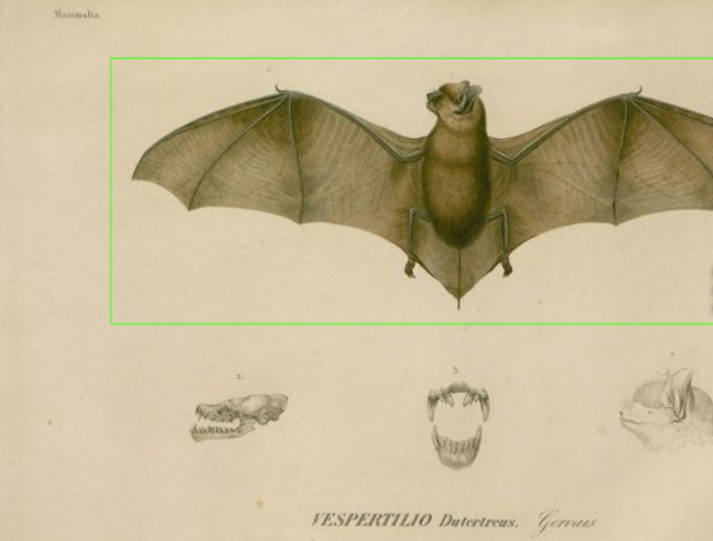
\includegraphics[height=4.5cm]{images/vhs_edge_case1.png}
			\subcaption{Annotation incomplète des illustrations}
		\end{subfigure}
		\hspace{1pt}
		\begin{subfigure}{0.30\linewidth}
			\centering
			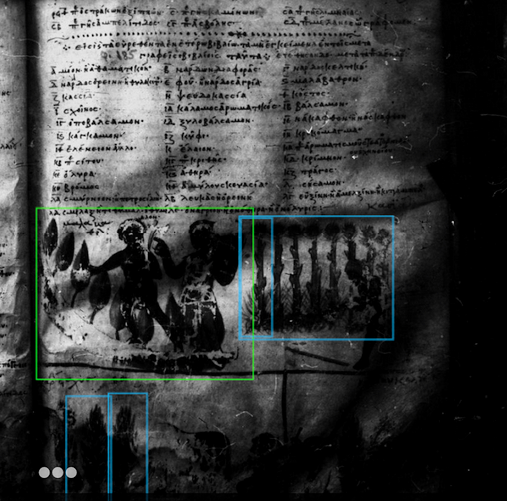
\includegraphics[height=4.5cm]{images/vhs_edge_case2.png}
			\subcaption{Annotation d'un document mal numérisé}
		\end{subfigure}
		\hspace{1pt}
		\begin{subfigure}{0.25\linewidth}
			\centering
			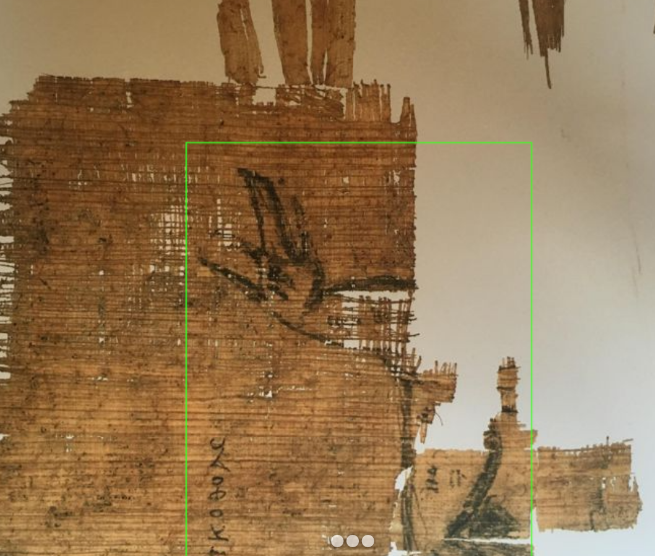
\includegraphics[height=4.5cm]{images/vhs_edge_case3.png}
			\subcaption{Annotation d'un document lacunaire}
		\end{subfigure}
		\caption{Cas limites rencontrés lors de l'annotation des images du projet \vhs}
		\label{fig:edge_cases_vhs}
	\end{figure}

	Ces décisions quant à l'annotation sont ainsi prises suite à un dialogue entre les équipes de chercheurs en vision et d'historiens, pour trouver un juste équilibre entre attentes et possibilités réelles. Des choix sont faits pour tirer parti des méthodes de vision artificielle, tout en acceptant que leurs résultats ne seront jamais identiques à ceux d'un travail manuel\footnote{De plus, un travail automatique présente des résultats uniformes et prévisibles, alors que les choix faits par des chercheurs varient selon les pratiques de chacun.} : les décisions doivent ainsi être prises pour exploiter de manière pertinentes ces techniques. Les pratiques définies par ces discussions entre les équipes mènent à des normes d'annotation : des spécifications sont alors rédigées pour les établir, et s'assurer de leur application uniforme, pour la création de données cohérentes.

    \subsubsection{Guides des pratiques : établir les normes}
	Pour s'assurer de l'application uniforme des normes d'annotation, il est de bonne pratique de rédiger une documentation à destination des chercheurs, à laquelle chacun peut se référer lors des étapes de création des données d'entraînement, qui constituent en elles-mêmes un travail considéré comme travail de recherche, puisqu'il requiert une connaissance et une compréhension des sources. Ainsi, les données produites suivent les mêmes règles, et cette cohérence assure une uniformité de jeu de données fourni au modèle de vision : cette uniformité permet, si une nouvelle étape d'entraînement est nécessaire, de corriger plus facilement les choix ayant mené à des résultats non-satisfaisants.
	
	Les chercheurs du projet \eida se sont vus fournir un \textit{Annotation Tutorial} en anglais, rédigé par Ségolène Albouy, cheffe de projet numérique, et Jil Le Bois, stagiaire de licence. Cette documentation fait suite à la mise en place d'une chaîne de traitement automatique des sources déposées par les chercheurs sur l'application du programme, qui produit une première détection que les chercheurs ont ensuite pour devoir de corriger. Le tutoriel qui a été communiqué contient des explications sur l'annotation dans l'application, avec un pas-à-pas détaillant chaque étape de ce travail, ainsi qu'une liste de cas pratiques établie en communication avec les historiens et l'équipe du laboratoire \imagine.
	
	Les cas pratiques établis répondent -- le plus souvent -- à des questions posées par les historiens à l'équipe d'ingénierie à l'occasion d'ateliers ou de séminaires, qui permettent de souligner au préalable les possibles doutes qui seront rencontrés lors de l'annotation. L'\textit{Annotation Tutorial} permet de garder trace de ces questionnements, et d'y apporter une réponse dont l'application sera systématique. La production de cette documentation, dont la responsabilité incombe aux ingénieurs d'étude, en tant que vecteurs de la communication entre les équipes d'histoire et de vision, pour donner à chaque parti impliqué la possibilité de se référer à un document qui rappelle les décisions prises. Cette possibilité de se référer à un document exhaustif est importante pour les étapes d'annotation, puisqu'elle garantit des données uniformes, mais aussi lors des étapes postérieures, notamment si d'autres entraînements sont nécessaires pour affiner les performances du modèle.

        	\\
        
        Le \dl et la vision artificielle permettent aux projets de recherche en histoire et en histoire de l'art d'envisager de nouvelles approches des sources, à l'aide de traitement automatisés qui offrent de nouvelles méthodes de navigation de corpus d'images massifs : de la détection à l'édition, les outils produits redéfinissent les étapes de traitement des sources, et il est ainsi nécessaire d'intégrer aux pratiques des chercheurs des méthodes spécifiques à ce type d'approche, et notamment pour la création de jeu de données d'entraînement, à la base du développement de tout modèle de \ml. Cette intégration passe notamment par la rédaction de documentation, ainsi qu'un dialogue entre les équipes de recherche en vision artificielle et les équipes d'historiens. Ce dialogue permet d'établir les besoins de chacun, et de développer des outils techniques qui répondent aux besoins scientifiques de manière pertinente, en développant des modèles qui, malgré leurs limites, rejoignent aux mieux les attentes des sciences historiques.
        \clearemptydoublepage


    \part{De l’image à l’objet : intégrer l’apprentissage profond au traitement des sources historiques}
        \chapter[L'apprentissage profond]{Principes et utilisation de l’apprentissage profond}
        L'apprentissage profond est un sous-domaine de l'apprentissage automatique basé sur l'apprentissage de couches successives de représentation. Le nombre de couches définit la profondeur du modèle : de nos jours, l'apprentissage profond compte plusieurs dizaines à plusieurs centaines de couches, qui apprennent toutes automatiquement à l'aide de données d'apprentissage\footcite{cholletApprentissageProfondAvec2020a}. Cette approche est au cœur des modèles de vision artificielle dont nous parlons dans ce mémoire, qui reposent sur des réseaux de neurones qui constituent ces couches superposées permettant un apprentissage des représentations à partir de données fournies.
        
            \section{\label{neuralNets}Réseaux de neurones et \textit{computer vision}}
                % Réseaux de neurones et computer vision

	\subsection{Des \og neurones \fg pour le \dl}
	Les modèles de vision artificielle pour des tâches telles que la détection d'objets, la détection de similarités ou la détection de lignes reposent souvent, en leur cœur, sur des réseaux de neurones plus ou moins profonds. Un réseau de neurones artificiels est un modèle paramétrique plus ou moins complexe\footcite{azencottIntroductionAuMachine2018} composé d'une couche d'entrée recevant les données brutes, puis d'une ou de plusieurs couches de calcul traitant les données en se corrigeant mutuellement, et d'une couche de sortie proposant une prédiction à partir des données d'entrée et des calculs effectués. Un réseau de neurones est dit \og profond \fg lorsqu'il compte un nombre suffisant, variable, de couches\footcite{azencottIntroductionAuMachine2018}. La prédiction se fait à l'aide d'un système de poids, qui correspondent aux paramètres d'une couche pour la transformation qu'elle applique aux données d'entrée\footcite{cholletApprentissageProfondAvec2020a}, et qui a pour objectif de calculer la prédiction la plus juste, c'est-à-dire d'associer l'entrée avec une cible\footnote{Pour un algorithme de détection d'images dans les manuscrits, l'entrée est l'image de la page, et la cible est l'étiquette \og Illustration \fg qui sera attribuée à la zone de l'image où une illustration est détectée.} par une série de transformations. L'algorithme corrige ses poids en cas de prédiction fausse : il s'agit de l'apprentissage, qui signifie donc la recherche d'un ensemble de valeurs pour les poids de toutes les couches du réseau de sorte que les résultats obtenus soient satisfaisants.
    
    \subsection{Réseaux de neurones à convolution}
    Les modèles mis en avant dans ce mémoire de recherchent reposent tous plus précisément sur des réseaux de neurones à convolution, ou \cnn, développés pour reconnaître des motifs visuels dans des images avec un minimum de traitements appliqués. Ces derniers sont favorisés pour les tâches de vision par ordinateur, et pour les tâches de perception en général\footcite{cholletApprentissageProfondAvec2020a} Ces réseaux sont composés de deux types de neurones agencés en plusieurs couches : les neurones de traitement, dédiés à traiter chacun une portion de l'image, et les neurones de mise en commun des sorties, dits de \textit{pooling}\footcite{goodfellowDeepLearning2016}. Les couches de convolution\footnote{Une couche de convolution est une couche constituée de copies d'un même neurone qui ne prend en compte qu'une partie le l'entrée.} ont pour spécificité d'être basées sur des fragments qui ne représentent que quelques pixels des images d'origine\footnote{Ces motifs locaux peuvent être les bords, les textures, et d'autres éléments. \cite{cholletApprentissageProfondAvec2020a}} : elles apprennent des motifs locaux, à l'inverse des couches entièrement connectées qui apprennent des motifs globaux. Les \cnn ont besoin de moins d'exemples d'apprentissage, parce qu'ils ont la capacité d'apprendre un motif et de le reconnaître quelle que soit sa position. Les \cnn requièrent donc un volume de mémoire moins important, pour une efficacité supérieure\footcite{goodfellowDeepLearning2016}. 
    
    Les \cnn ont la capacité d'apprendre des motifs locaux, puis d'apprendre dans les couches suivantes des motifs plus grands qui en découlent, apprenant ainsi des concepts visuels de plus en plus abstraits, et de plus en plus complexes\footcite{cholletApprentissageProfondAvec2020a} : l'intérêt dans le cadre d'un apprentissage pour la vision artificielle réside donc dans cette possibilité d'apprendre des motifs invariants par translation\footnote{\og  L'invariance par translations est une propriété fondamentale partagée par la quasi-totalité des opérations de traitement d'images. Elle exprime le fait qu'une information visuelle sera traitée de la même façon, quelle que soit sa localisation dans l'espace. En effet, si on bouge le capteur, chaque objet sera déplacé dans l'image, mais devra être traité de la même façon que précédemment. \fg \cite{ronseInvarianceParTranslations}} et spatialement hiérarchiques, deux caractéristiques fondamentales du monde visuel\footcite{cholletApprentissageProfondAvec2020a}.


        
            \section[Modèles de vision \textit{off-the-shelf}]{Modèles de détection \textit{off-the-shelf} : outils libres pour l'extraction d’objets}
                % Modèles de vision off-the-shelf : outils libres pour la détection d’objets

\subsection{YOLOv5, \docex et autres modèles}
    \subsubsection{Utilisation d'un modèle pré-entraîné}
	Il est courant, pour la vision artificielle, d'utiliser un modèle pré-entraîné sur un grand jeu de données peu spécifique, et de l'affiner à partir d'un plus petit jeu de données correspondant précisément aux attentes et applications du modèle dans le projet\footnote{Nous nous focaliserons spécifiquement sur les modèles de détection et de classification, dont la question de l'entraînement a été abordée lors du stage.}. En effet, un modèle entraîné sur un jeu de données de base suffisamment large et généraliste apprend des caractéristiques qui peuvent être appliquées à l'ensemble du monde visuel, et peut ainsi servir de modèle générique pour de nombreux problèmes de vision par ordinateur\footcite{cholletApprentissageProfondAvec2020a}, même si ces derniers sont éloignés de la tâche initiale. La portabilité des caractéristiques apprises rend ainsi l'usage du \dl pertinent dans le cadre de projets de recherche sur des sources historiques, puisqu'elle assure ainsi l'efficacité des modèles créés malgré les possibles limites des jeux de données disponibles : il est ainsi possible d'entraîner un modèle sur un jeu de données limité, qui correspond à la réalité matérielle des sources étudiées. 
	
	\subsubsection{ImageNet} 
	ImageNet\footcite{ImageNet} est une initiative ayant pour objectif de fournir en accès libre un vaste jeu de données images pour la recherche en vision artificielle. Cette initiative est née du besoin crucial de données d'entraînement et de validation pour le \ml, et particulièrement pour la classification, tâche de base de la vision par ordinateur, qui requiert un volume important d'images pour l'obtention de bonnes performances. Le jeu de données ImageNet compte plus d'un million d'images, catégorisées selon des concepts récupérés du projet WordNet qui vise à répertorier et classifier le contenu sémantique et lexical de la langue anglaise. Chaque image du jeu de données est annoté manuellement pour indiquer les objets présent dans l'image : ImageNet est un projet participatif, ce qui permet d'assurer la continuité de son enrichissement. Le projet ne possède pas les droits des images du jeu de données, formulant simplement une liste d'images disponibles sur le Web pour chaque concept WordNet : elles sont mises à disposition des projets à visée non-commerciale, pour assurer aux chercheurs la possibilité de mener des recherches en ayant accès à un jeu de données d'entraînement riche et vaste, permettant de développer des modèles performants avant un entraînement plus spécialisé.
    
    \subsubsection{\yolov : un modèle de pointe pour l'extraction d'objets}
	\yolov\footcite{ultralyticsUltralyticsYOLOv8Docs} est la cinquième version du modèle de détection d'objets et de segmentation d'images \yolo, développé à l'Université de Washington Joseph Redmon et Ali Farhadi et lancé en 2015. \yolov, publié en 2020, est un modèle réputé pour sa rapidité d'exécution et sa précision\footcite{buttnerCorDeepSacroboscoDataset2022}, pré-entraîné sur le jeu de données MS COCO\footcite{COCOCommonObjects}, dont l'implémentation se veut aisée : \yolov, contrairement à ses prédécesseurs, est directement implémenté dans PyTorch\footcite{PyTorch}, permettant une intégration facile à un environnement de développement, puisqu'il nécessite moins d'adaptation que les versions précédentes fonctionnant avec le \textit{framework} Darknet\footcite{DarknetOpenSource}, basé sur le langage C\footcite{sharmaTrainingYOLOv5Object2022}. Le réseau neuronal de \yolo fonctionne en trois étapes : l'extraction de caractéristiques des données d'entrée, l'agrégation de ces caractéristiques, puis la résolution du problème (dans ce cas précis, la détection des objets)\footcite{buttnerCorDeepSacroboscoDataset2022} Le modèle est disponible en accès libre, et constitue ainsi une base solide pour les projets souhaitant utiliser un modèle de détection d'objets : \yolov peut, en effet, être entraîné sur un jeu de données choisi, pour en affiner la détection et l'appliquer à des images plus spécifiques, telles que des pages d'ouvrages.
	
	Les projets \eida et \vhs entraînent, pour la détection d'illustrations dans les numérisations d'ouvrages, des modèles ayant pour base \yolov. Sans entraînement spécifique, en s'appuyant exclusivement sur le pré-entraînement fait avant la mise en ligne du modèle, les performances sont peu satisfaisantes : les jeux de données utilisés pour ce pré-entraînement, qu'il s'agisse d'ImageNet ou de MS COCO, sont en effet des jeux de données d'images réelles, faits pour l'apprentissage de la classification d'objets du quotidien, et ne sont donc initialement pas adaptés à la segmentation de pages de manuscrits ou à la détection d'illustrations. Il faut ainsi compter sur les propriétés de portabilité de l'apprentissage, qui assurent que ce pré-entraînement sur des images réelles permet d'accélérer le processus de développement du modèle, puisqu'elles permettent de s'intéresser immédiatement à l'entraînement à partir de données spécifiques, et réduisent le volume nécessaire. 
	
	\subsubsection{\docex : un modèle pour les sources historiques}
   	\docex est un modèle \textit{off-the-shelf} de détection d'objet, dédié spécifiquement aux documents historiques\footcite{monnierDocExtractorOfftheshelfHistorical2020}. Développé par Tom Monnier, ce modèle a pour vocation d'être un outil efficace et prêt à l'usage pour le traitement de documents numérisés, capable de détecter le texte et segmenter les lignes, et d'extraire les illustrations en détectant leurs contours précis\footnote{Contrairement à \yolov qui produit des annotations rectangulaires et ne gère pas les polygones.}. \docex est entraîné à partir d'images produites par un générateur de documents historiques synthétiques (fig. \ref{fig:syndoc}), qui promet de bonnes performances même sans \textit{fine-tuning} : l'utilisation de ce générateur automatique, appelé SynDoc\footnote{Les images générées par SynDoc sont composées aléatoirement à partir d'une sélection d'images de fonds (pages et contextes), auxquelles sont ajoutées une mise en page selon laquelle est disposé un contenu image et texte, puis du bruit. Tous ces éléments sont tirés d'un jeu d'images pré-établi (constitué de 177 images de pages, 15 contextes, plus de 8000 œuvres d'art provenant de WikiArt, des lettrines générées à partir d'une lettre aléatoire avec 91 fonts possibles, et des dessins, schémas et textes tirés d'articles aléatoires sur Wikipedia, avec plus de 400 fonts) et composent des pages aléatoires mêlant images, texte et bruit, avec un nombre vaste de possibilités qui égale les plus grands jeu de données d'entraînement. Ces pages ne nécessitent pas d'annotations manuelles, puisque chaque élément de contenu est pré-annoté.}, vise à répondre aux problématiques de création de jeux de données d'entraînement à partir de documents historiques, limités à la fois par le nombre de documents disponibles et les moyens humains que l'annotation d'images nécessite. SynDoc permet ainsi, dans la création d'un modèle, de combler l'absence d'un jeu de données de grande échelle d'images de documents historiques annotées\footcite{buttnerCorDeepSacroboscoDataset2022}.
   	
   	\begin{figure}[h]
   		\centering
   		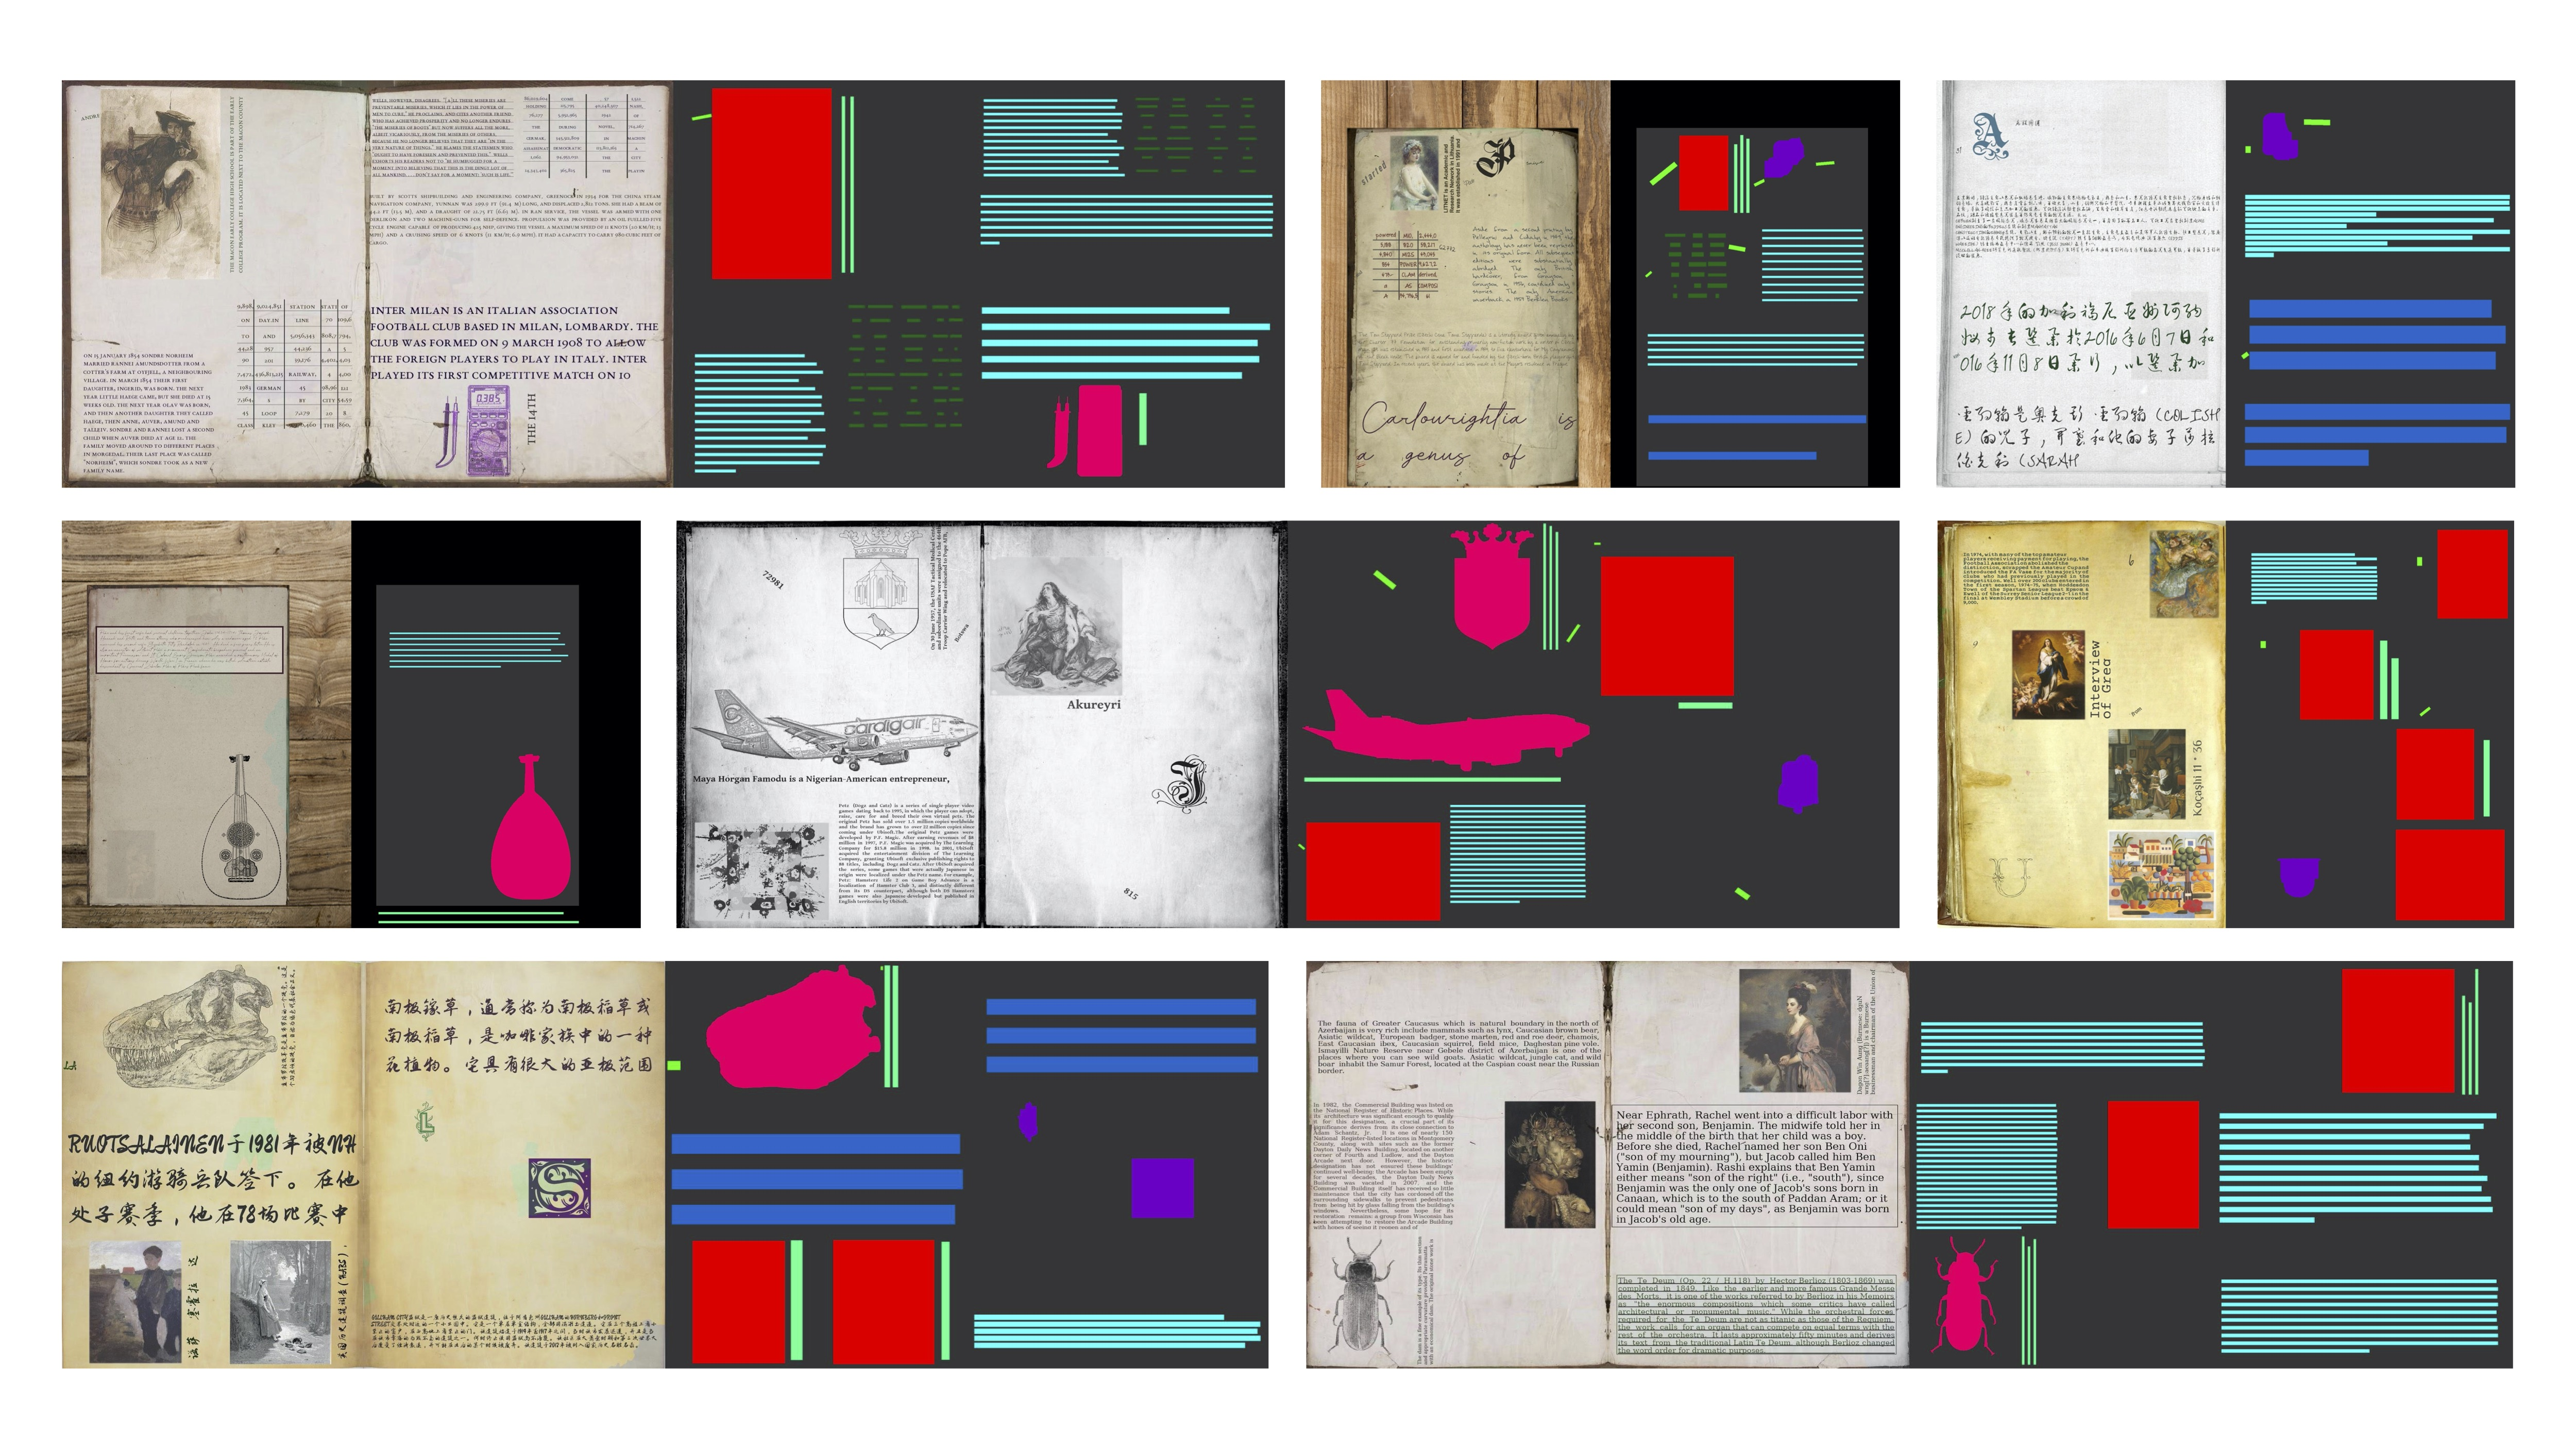
\includegraphics[width=13cm]{images/syndoc.jpg}
   		\caption{Exemples tirés d'un jeu de données généré avec SynDoc}
   		\label{fig:syndoc}
   	\end{figure}
   	
   	Contrairement à \yolov, \docex est donc développé spécifiquement pour le traitement des sources historiques, en prenant en compte les spécificités de ces documents iconographiques : le modèle est ainsi adapté au traitement d'images de pages contenant du texte et des illustrations, et prévoit également des outils de traitement du texte, tels que la détection des lignes en prévision\footnote{La détection des lignes est une étape préliminaire de traitements tels que la reconnaissance optique de caractères (OCR) ou la reconnaissance de l'écriture manuscrite (HTR).}. \docex semble ainsi être le modèle à favoriser dans le cadre des projets mentionnés dans ce mémoire, cependant, les premières évaluations des modèles\footnote{Les deux modèles ont fait l'objet d'un entraînement préliminaire sur des sources historiques qui ne sont cependant pas celles des deux projets, pour un premier affinement de leurs performances.} sur les sources d'\eida et de \vhs semblent témoigner de performances équivalentes.
   	
   	En effet, les détections de diagrammes lancées sur des sources du corpus \eida en prévision de leur annotation par les chercheurs pour la constitution du jeu d'entraînement ont témoigné de performances prometteuses aussi bien pour \docex que pour \yolov  (fig. \ref{fig:performances_modeles}), avec des diagrammes non-détectés dans les deux cas : les performances de chacun des deux modèles varient en fonction des pages, et il sera donc nécessaire de les départager en évaluant plus précisément leurs performances en amont de l'entraînement, puis après un premier entraînement des deux modèles sur les sources du projet\footnote{Sur le projet \eida, les modèles ont été fournis par les chercheurs du laboratoire \imagine et l'ingénieur du projet \vhs, n'ont donc pas encore été évalués sur les sources astronomiques du projet. La vérité de terrain étant encore en cours de production à l'été 2023, l'évaluation sera faite à partir d'un fragment de ce jeu de données lorsqu'il sera disponible.}. En tant que modèles \textit{off-the-shelf} en libre accès, \yolov et \docex ont pour vocation d'être efficaces et performants même sans entraînement sur des données spécifiques, et permettent ainsi de mener de manière satisfaisante des tâches de détection et d'extraction sur des données personnelles. Cependant, pour obtenir de meilleures performances, il est préférable d'entraîner ces modèles \textit{off-the-shelf} sur des images tirées du corpus du projet, pour l'adapter et le spécialiser dans la résolution de ces problèmes particuliers.
   	
\subsection{Entraînement et \textit{fine-tuning} d'un modèle de détection}
    \subsubsection{Démarche et volume des données}
	L'entraînement d'un modèle sur un jeu de données spécifiques permet de préciser les tâches effectuées et d'obtenir un modèle adapté aux besoins spécifiques de chaque projet. L'utilisation d'un modèle pré-entraîné permet, comme mentionné précédemment, de pallier aux limites de jeux de données avec trop peu d'exemples, en exploitant les représentations apprises précédemment et en les spécialisant sur les données spécifiques du projet qui l'utilise.
	
	\begin{figure}[H]
		\begin{subfigure}{1\linewidth}
			\centering
			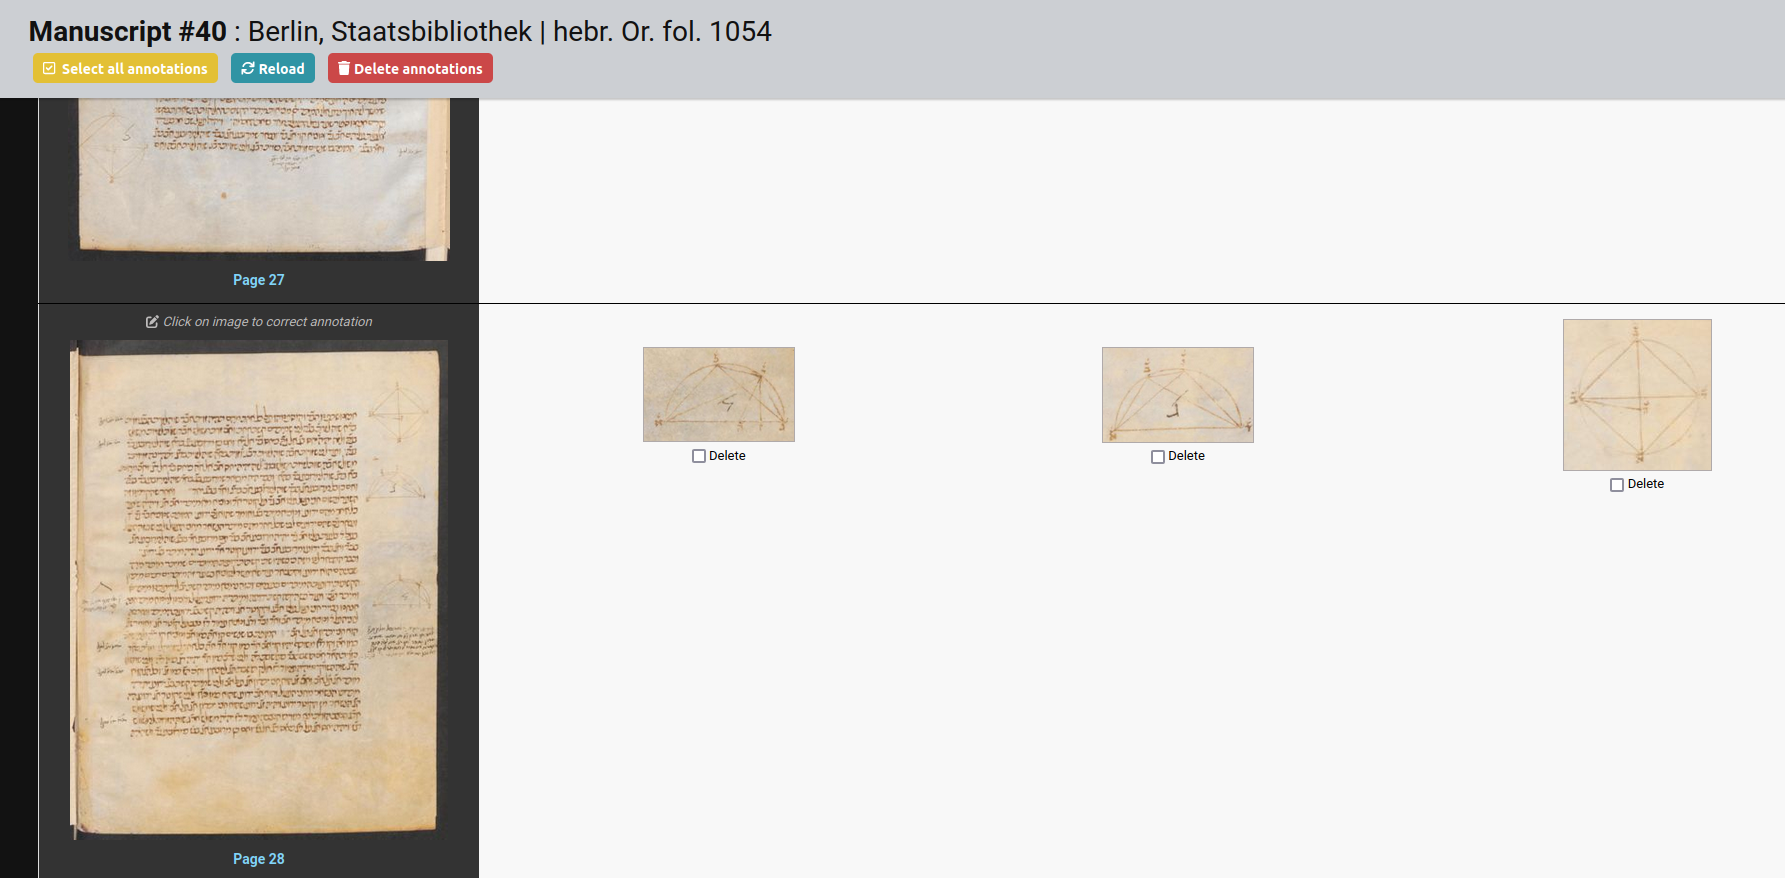
\includegraphics[width=10cm]{images/ms40_p28_docext.png}
			\subcaption{p. 28, \docex}
		\end{subfigure}
		\hspace{1pt}
		\begin{subfigure}{1\linewidth}
			\centering
			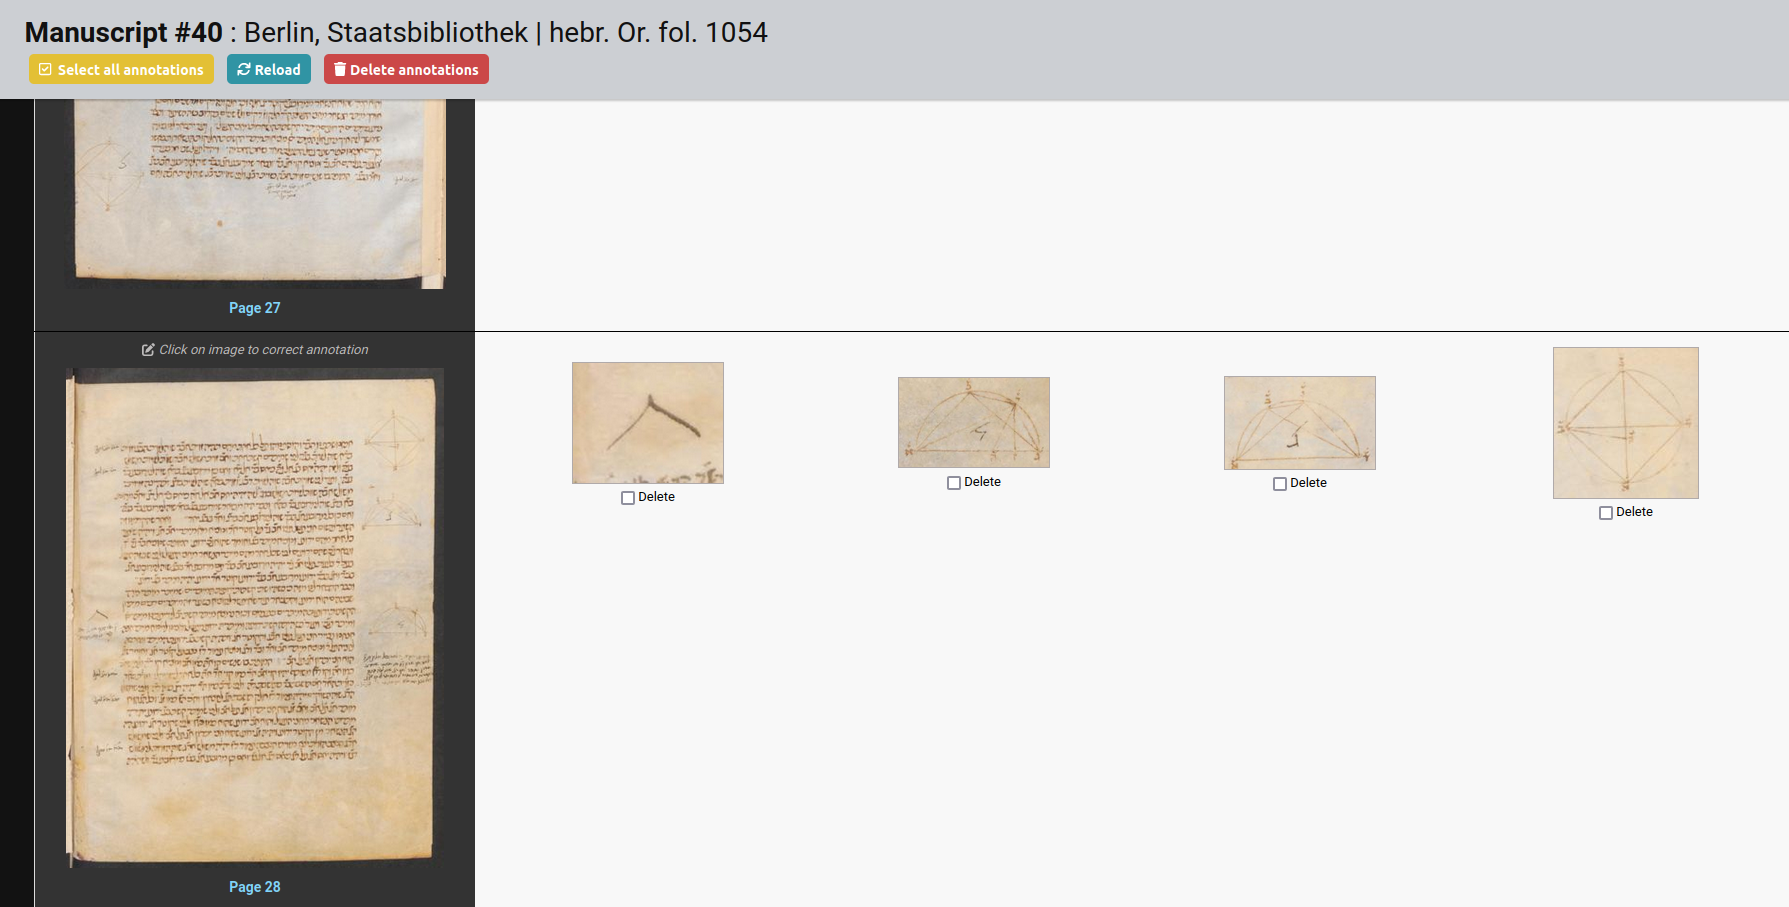
\includegraphics[width=10cm]{images/ms40_p28_yolov5.png}
			\subcaption{p. 28, \yolov}
		\end{subfigure}
		\begin{subfigure}{1\linewidth}
			\centering
			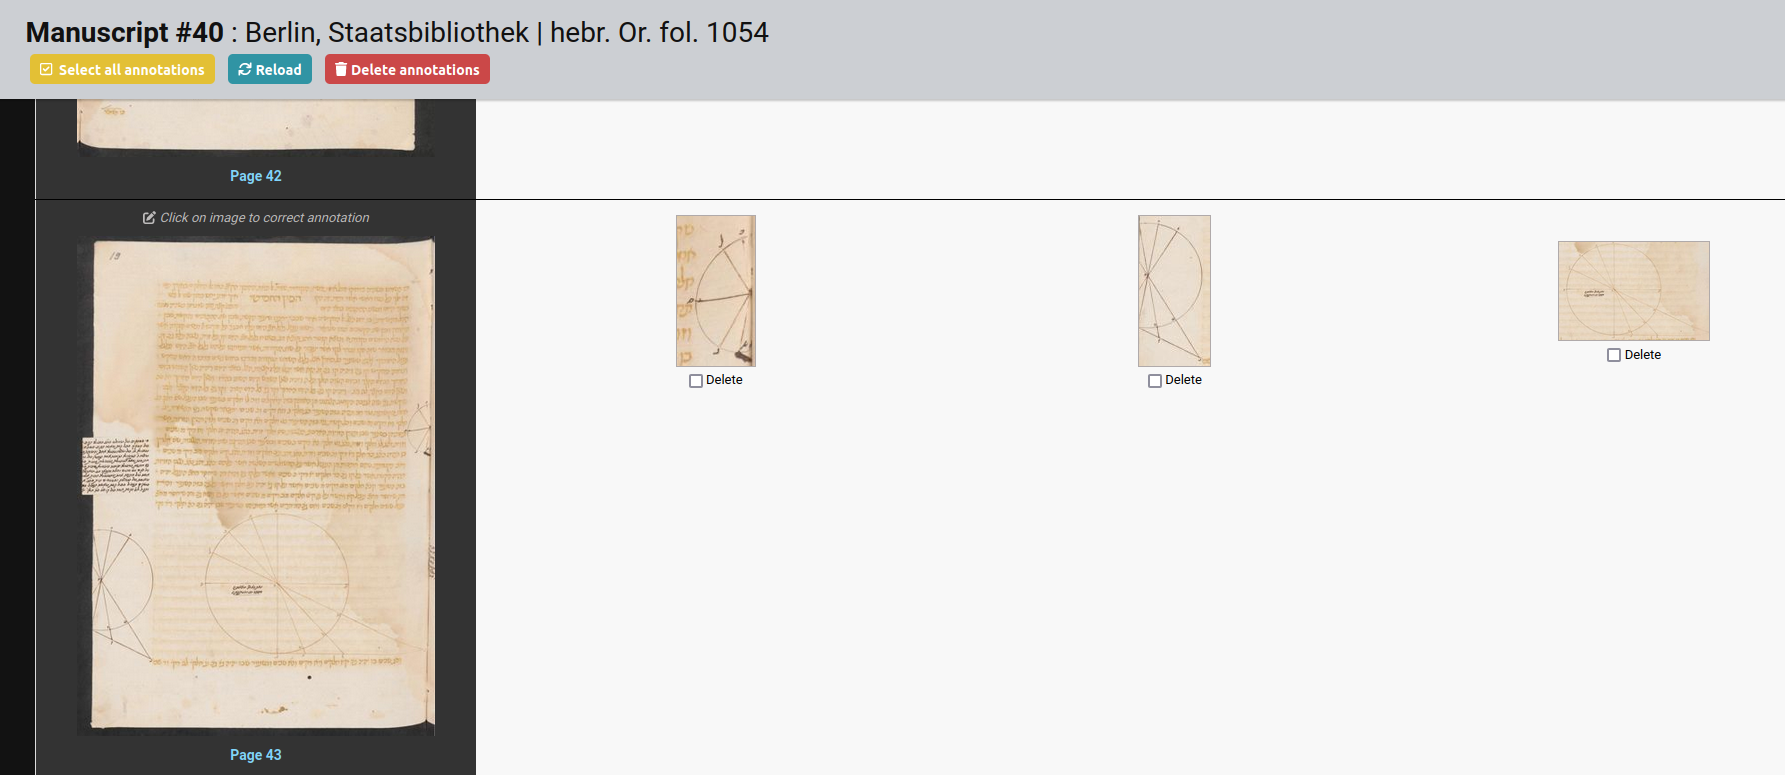
\includegraphics[width=10cm]{images/ms40_p45_docext.png}
			\subcaption{p. 45, \docex}
		\end{subfigure}
		\hspace{1pt}
		\begin{subfigure}{1\linewidth}
			\centering
			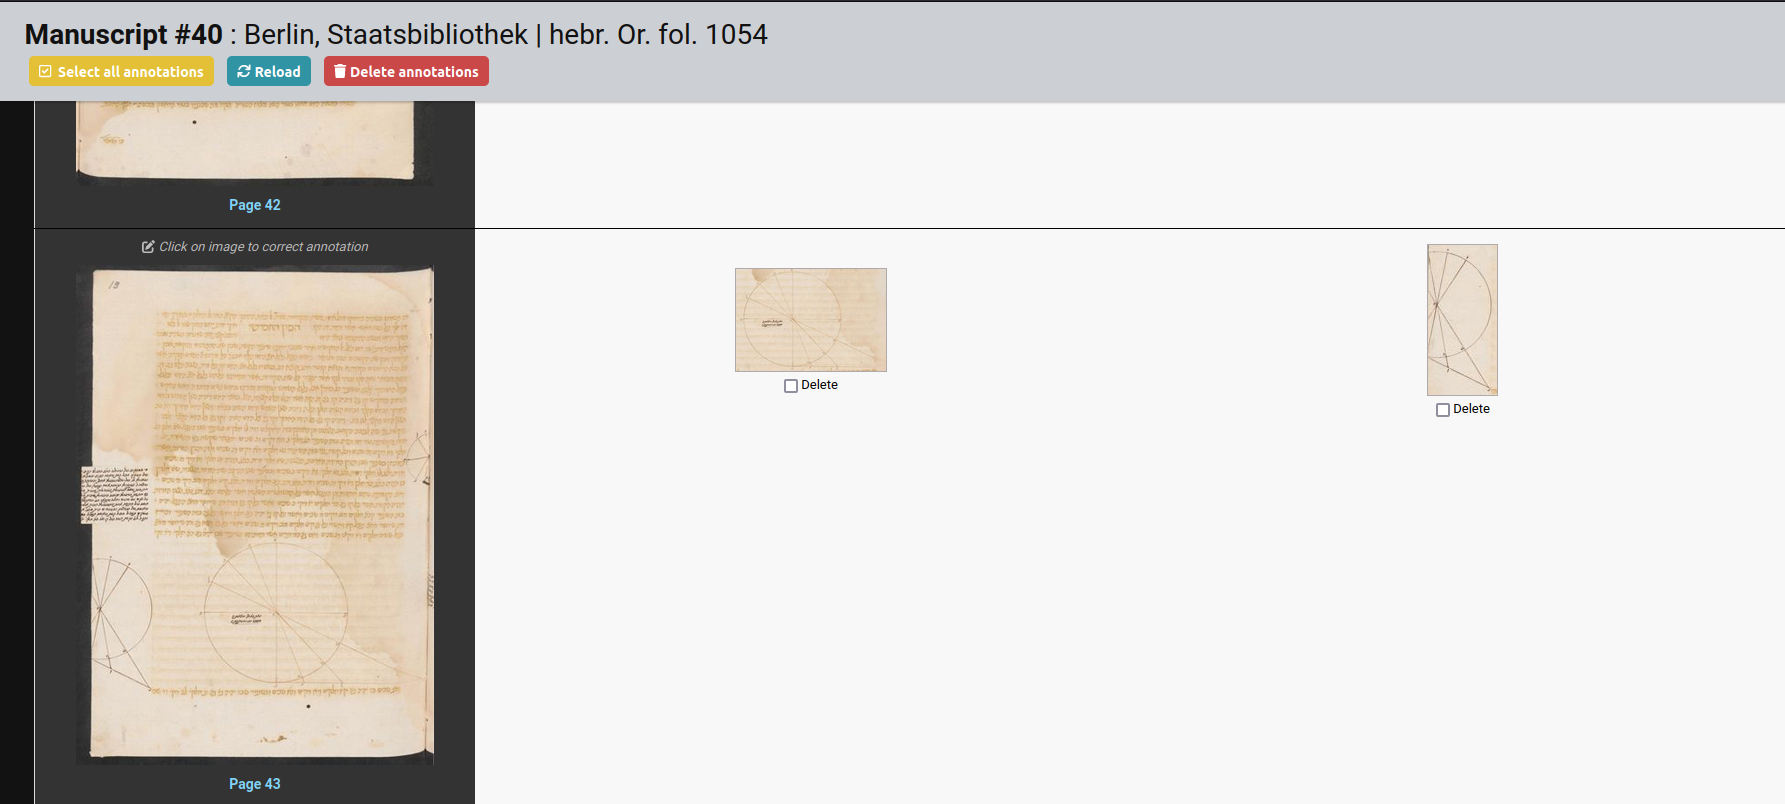
\includegraphics[width=10cm]{images/ms40_p45_yolov5.png}
			\subcaption{p. 45, \docex}
		\end{subfigure}
		\caption{Diagrammes détectés par les modèles \yolov et \docex dans deux pages du manuscrit hebr. Or. fol. 1054 de la Staatsbibliotek (Berlin).}
		\label{fig:performances_modeles}
	\end{figure}

	Les modèles de détection \textit{off-the-shelf} comme \yolov prévoient souvent un \textit{workflow} pour l'entraînement du modèle\footcite{sharmaTrainingYOLOv5Object2022} par des projets qui souhaiteraient le spécialiser. Ainsi, dans le cas de \yolov, l'entraînement étant prévu par les développements mis à disposition par Ultralytics, il est nécessaire pour les ingénieurs de prévoir des jeux de données d'entraînement adaptés au format requis par le modèle\footnote{Les projets \vhs et \eida emploient tous deux \yolov comme modèle, ou \docex intégré au \textit{workflow} développé par Ultralytics pour \yolov : la structure des jeux de données d'entraînement est donc la même pour les deux modèles.} : l'annotation par les chercheurs doit donc être effectuée en prenant en compte ces restrictions, et les outils développés par les ingénieurs pour l'annotation des images doivent avoir pour sortie des fichiers aux formats appropriés. Un document de spécification sur les formats d'image et d'annotation a été réalisé dans le cadre du projet \eida (Annexe \ref{YOLOv5Training}), pour garder traces des besoins techniques de l'entraînement, étape suivante du projet. 
	
	L'entraînement d'un modèle \yolov se fait à partir d'un \textit{dataset} d'images et d'étiquettes (\textit{labels}) : il s'organise ainsi en un dossier de fichiers image (au format .png ou .jpg), et un dossier de fichiers texte (au format .txt) contenant une liste d'objets. Chaque fichier texte correspond à un ou plusieurs fichiers image -- plusieurs dans le cas de numérisation d'ouvrages, notamment, qui se composent d'un fichier d'annotations par ouvrage numérisé et non par image -- et listent les objets détectés dans l'image, à raison d'une ligne par objet. L'objet est caractérisé par ses dimensions (selon un rectangle qui l'encadre) et ses coordonnées sur l'image. Par exemple, le fragment de ficher d'annotation suivant correspond aux quatre objets détectés sur la page 6 du manuscrit 5 (Alm. 1) de la Gurukul Kangri Haridwar Collection (fig. \ref{fig:annotation_ms143}) :
	
	\begin{lstlisting}
		6 ms143_0006.jpg
		243 1852 464 549
		168 7 763 618
		440 951 1174 1130
		919 47 851 826\end{lstlisting}

   	\begin{figure}[H]
		\centering
		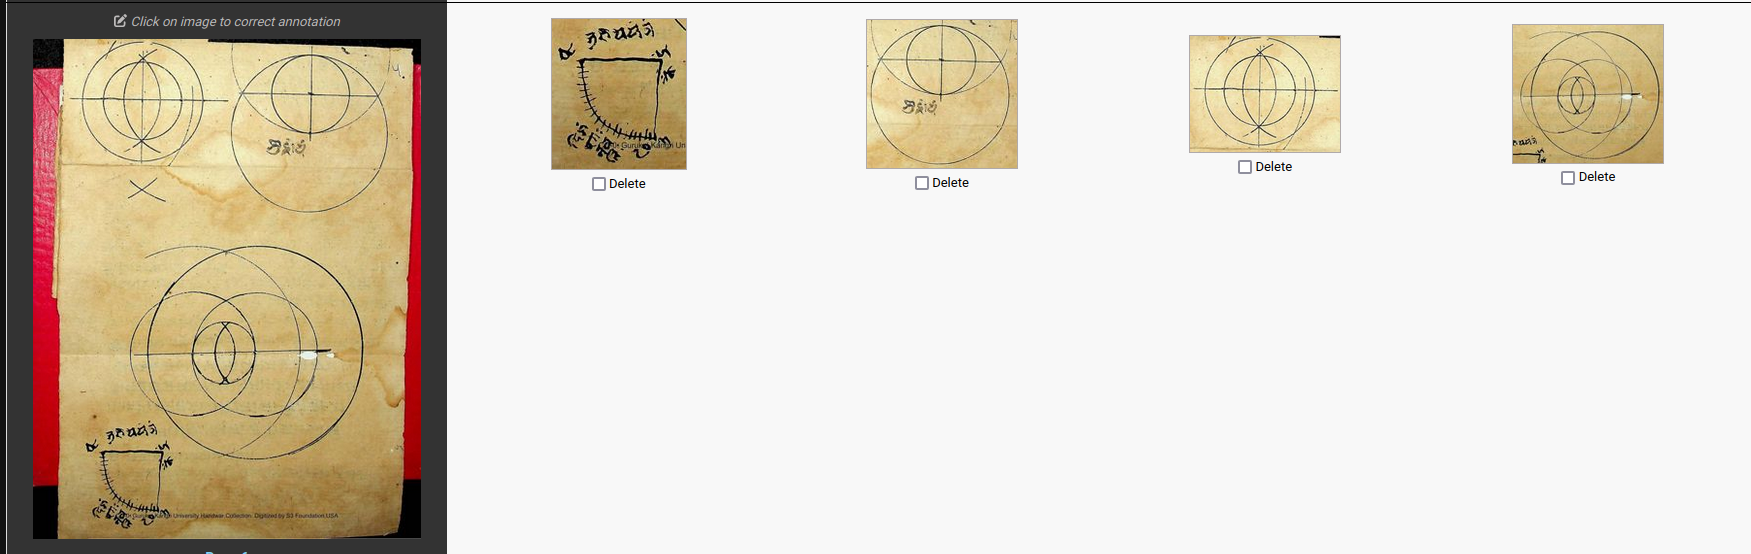
\includegraphics[width=15cm]{images/ms143_p6.png}
		\caption{Objets détectés sur la page 6 du manuscrit 5 (Alm. 1) de la Gurukul Kangri Haridwar Collection }
		\label{fig:annotation_ms143}
	\end{figure}

	À partir de cet ensemble d'images et d'annotations, l'entraînement peut être effectué : \yolov prévoit un script pour l'entraînement d'un modèle, dont seuls les paramètres doivent être modifiés pour l'adapter aux besoins du projet. Ainsi, les modèles de détection \textit{off-the-shelf} tels que \yolo ou \docex prévoient la possibilité d'un entraînement, simplifié par la mise à disposition d'outils permettant d'effectuer cette étape en écrivant peu de code. Cette volonté de rendre accessible des outils adaptables, construits comme un socle solide pour des objectifs variés, permet l'intégration de la vision artificielle à des projets divers, sans demander de ces derniers de créer ou d'entraîner de zéro des réseaux de neurones ou des modèles de détections. La détection étant, en effet, une tâche de base de la vision par ordinateur, il est peu pertinent d'allouer des ressources pour reproduire des techniques déjà appliquées par de nombreux projets, et les outils \textit{off-the-shelf} offrent donc la liberté d'envisager la vision artificielle comme élément d'une chaîne de traitement des sources en allégeant les besoins et ressources -- notamment humains et temporels -- que demandent le développement et l'application de ces techniques. 

    \subsubsection{Sur-ajustement et diversité des exemples}
	
	L'utilisation d'un modèle pré-entraîné permet d'obtenir un modèle de détection fonctionnel malgré une faible quantité de données disponibles, puisque celui-ci a la capacité de généraliser les caractéristiques apprises à partir des données de pré-entraînement et de les appliquer aux données spécifiques du projet. Un trop faible volume de données présente en effet le risque de produire un modèle peu performant à cause du sur-ajustement (ou \textit{overfitting})) : on parle de sur-ajustement lorsqu'un modèle est bien ajusté aux données d'entraînement, mais incapable de généraliser face à de nouvelles données\footcite{cholletApprentissageProfondAvec2020a}. 
	
	Il est crucial de prévoir, lors de la constitution du jeu de données d'entraînement, une portion dédiée à la validation : on considère généralement que 20\% du jeu de données total est un volume suffisant pour cette étape. Les données de validation sont des données -- dans le cas de la détection, des images et annotations produites par des humains -- qui n'ont jamais été vues par le modèle et n'ont donc pas été utilisées pour l'entraînement. Comme les données d'entraînement, ces données de validations doivent être représentatives et diversifiées, puisqu'elles permettent de vérifier les performances du modèles, et d'identifier un sur-ajustement si le modèle ne donne pas, après entraînement, des résultats satisfaisants sur cet ensemble. Les données de validation permettent de mettre en avant les pertes à mesure que le modèle s'ajuste aux données d'entraînement\footcite{carremansHandlingOverfittingDeep2019}.
	
	Pour prévenir le sur-ajustement d'un modèle\footnote{Il existe diverses méthodes pour corriger le sur-ajustement d'un modèle de détection après entraînement, cependant, ce mémoire traitant de l'intégration de la vision artificielle à une chaîne de traitement des sources par le prisme du lien avec les équipes de recherche en histoire, nous n'aborderons pas ces questions qui concernent plus spécifiquement les aspects techniques de la création d'un modèle de détection. \cite{carremansHandlingOverfittingDeep2019}}, il est nécessaire de prévoir un jeu de données d'entraînement au volume suffisant -- supérieur à plusieurs milliers d'exemples dans le cas d'images\footnote{Le projet \eida compte plusieurs dizaines de milliers de pages dans son jeu de données d'entraînement.} -- et à la diversité représentative des données que le modèle pourra rencontrer. Le modèle de détection entraîné présente une capacité de généralisation qui rend son application pertinente pour le traitement des sources : l'entraînement d'un modèle \textit{off-the-shelf} permet ainsi de partir d'un modèle relativement performant dans des contextes variés et d'obtenir un modèle répondant aux besoins du projet, en trouvant l'équilibre entre manque d'ajustement et sur-ajustement.
        	\\
		
		Les modèles de vision \textit{off-the-shelf} ouvrent à des projets divers la possibilité d'intégrer la vision artificielle à leurs méthodologies, en réduisant le coût humain et temporel du développement d'un modèle de \textit{deep learning} par la mise à disposition en accès libre d'outils déjà performants, qu'il est possible d'entraîner pour les ajuster à des données spécifiques. Pour la détection d'objet, des jeux de données en accès libre tels qu'ImageNet permettent un pré-entraînement de ces modèles \textit{off-the-shelf}, qui apprennent alors des caractéristiques générales qui peuvent être précisées par un entraînement sur des sources plus spécifiques, en nécessitant un volume de données moins important qu'un modèle créé de zéro. Ces modèles de détection \textit{off-the-shelf} présentent ainsi une solution aux limites que peuvent présenter les sources historiques en termes de volume des données disponibles, et permettent également aux projets de se construire sur des bases solides, sans allouer de ressources à la création d'outils déjà existants, déjà performants, pour des tâches telles que la détection d'objet qui font partie des tâches canoniques de la vision par ordinateur.
        \clearemptydoublepage
        
        \chapter[Construire une plateforme pour la détection]{Construire une plateforme pour la détection : outils, interfaces et modèles de données}
        L'intégration du \textit{deep learning} aux pratiques des chercheurs en sciences historiques passe par le développement d'une plateforme qui leur permet d'exploiter simplement ces outils pour traiter leurs sources. Cette plateforme à interface graphique doit être adaptée aux sources traitées, et pensée pour intégrer toutes les fonctionnalités souhaitées. En s'appuyant sur les développements réalisés par les projets \eida et \vhs, cette partie revient sur la construction d'une application  et d'une \api dédiées à la détection de diagrammes et images scientifiques dans les numérisations d'ouvrages manuscrits ou imprimés, avec une interface pour la correction de la détection : nous évoquons ainsi les méthodes de développement, les réflexions liées aux données, les besoins matériels liés à l'utilisation d'algorithmes de vision, et le développement d'une \api pour lancer l'inférence sur un \gpu. 
         
            \section{\label{detectionApp}Penser une application pour la détection d'objet}
                % Architecture de l’application : fonctionnalités et outils

\subsection{Une interface pour le dépôt des sources}
    \subsubsection{Sous-sous-section 1}
    
    \subsubsection{Sous-sous-section 2}

    
\subsection{Décrire les sources}
        \subsubsection{Sous-sous-section 1}

        \subsubsection{Sous-sous-section 2}


\subsection{Images et objets détectés : une nouvelle source ?}
        \subsubsection{Sous-sous-section 1}


        \subsubsection{Sous-sous-section 2}


        
            \section{Annoter sur un GPU : extractorAPI}
                % Annoter sur un GPU : extractorAPI

\exapi\footcite{norindrElementExtractionGPU2023} est une \api développée en tant que module de l'application \eida : elle a pour vocation de séparer l'algorithme de détection d'objets du reste de l'application. \exapi est conçue autour d'une unique fonctionnalité : exécuter un algorithme de détection d'objet sur des images reçue de l'application \eida, et retourner les résultats de cette détection.

\subsection{Architecture du système}
    \subsubsection{CPU ou GPU ?}
	L'apprentissage profond et la vision artificielle représentent le plus souvent des tâches qui requièrent une puissance de calcul importante. L'utilisation d'un \gpu plutôt que d'un \cpu est donc de bonne pratique, si ce n'est une nécessité, pour assurer la complétion des tâches en un temps correct, particulièrement lorsqu'il s'agit de tâches qui doivent retourner rapidement un résultat à un utilisateur. Un \gpu est un processeur conçu pour avoir de meilleures performances dans le traitement d'images, et dans l'exécution parallèle de tâches\footcite{sharabokWhyDeepLearning2020}, tandis qu'un \cpu est un processeur conçu pour effectuer des calculs plus basiques, pour répondre aux besoins quotidiens. Le nombre important de cœurs que contient un \gpu permet une gestion simultanée de nombreuses tâches, et permet donc une plus grande efficacité sur des traitements basés sur le parallélisme, comme le sont les réseaux de neurones, éléments centraux du \dl.
	
	D'un point de vue applicatif, l'utilisation d'un \gpu pour les tâches de vision artificielle permet d'assurer la fluidité du fonctionnement de l'application qui intègre ces algorithmes, et de retourner, comme mentionné précédemment, un résultat rapide à l'utilisateur qui souhaiterait soumettre ses sources à un traitement via l'application. Outre le \ml, un \gpu a les capacités de traiter les images de manière plus performante. Les traitements par des algorithmes de vision artificielle nécessitent en effet un enregistrement des images dans l'application pour que s'effectuent les tâches, ainsi, d'un point de vue matériel, il est essentiel de prévoir, d'une part, la mémoire nécessaire au stockage -- même s'il est temporaire -- des images, ainsi que la puissance de calcul pour leur enregistrement puis leur traitement dans un délai suffisamment court pour retourner une réponse à l'utilisateur en un temps satisfaisant. 
    
    \subsubsection{De l'utilisateur au modèle de détection}
	Les applications \vhs et \eida pour la détection d'objets dans les numérisations reposent sur une même architecture globale, construite pour être adaptable par des projets qui souhaiteraient traiter des sources historiques par la vision artificielle : dans une optique de programmation modulaire, et pour permettre l'utilisation d'un \gpu pour le traitement des images, la solution proposée par ces projets est l'exclusion du modèle de détection de la structure de l'application en elle-même, et le développement d'une \api sur un \gpu pour cette tâche spécifique.
	
	Ainsi, l'application est développée, avec ses dépendances, sur un serveur spécifique, qui accueille le code de l'application et la base de donnée PostgreSQL à laquelle elle est adossée, et stocke les images versées par les utilisateurs qui servent à la génération de manifestes \iiif propres à \eida. Par le biais de l'interface web, l'utilisateur envoie des requêtes à cette application, qui retourne des réponses à l'utilisateur. Le modèle de détection existe sur un serveur indépendant du serveur de l'application, sur un \gpu. Pour connecter le modèle à l'application, une \api est développée : celle-ci reçoit de la part de l'application \eida des requêtes contenant les informations soumises par l'utilisateur, et retourne à l'application une réponse, qui est ensuite retournée à l'utilisateur par son biais. Ainsi, le lien de l'utilisateur au modèle de détection se fait par le biais de l'application, elle-même liée au modèle par une interface qu'est l'\api (fig. \ref{fig:archi_eida}) : l'\api n'a pas d'interface destinée à être vue par l'utilisateur\footnote{Contrairement à l'application, composée d'un \textit{back end} et d'un \textit{front end}, l'\api n'est constituée que d'un \textit{back end}. Il n'existe ainsi pas d'interface accessible à l'utilisateur, seulement le code permettant son fonctionnement.}.
	
	\begin{figure}[h]
		\centering
		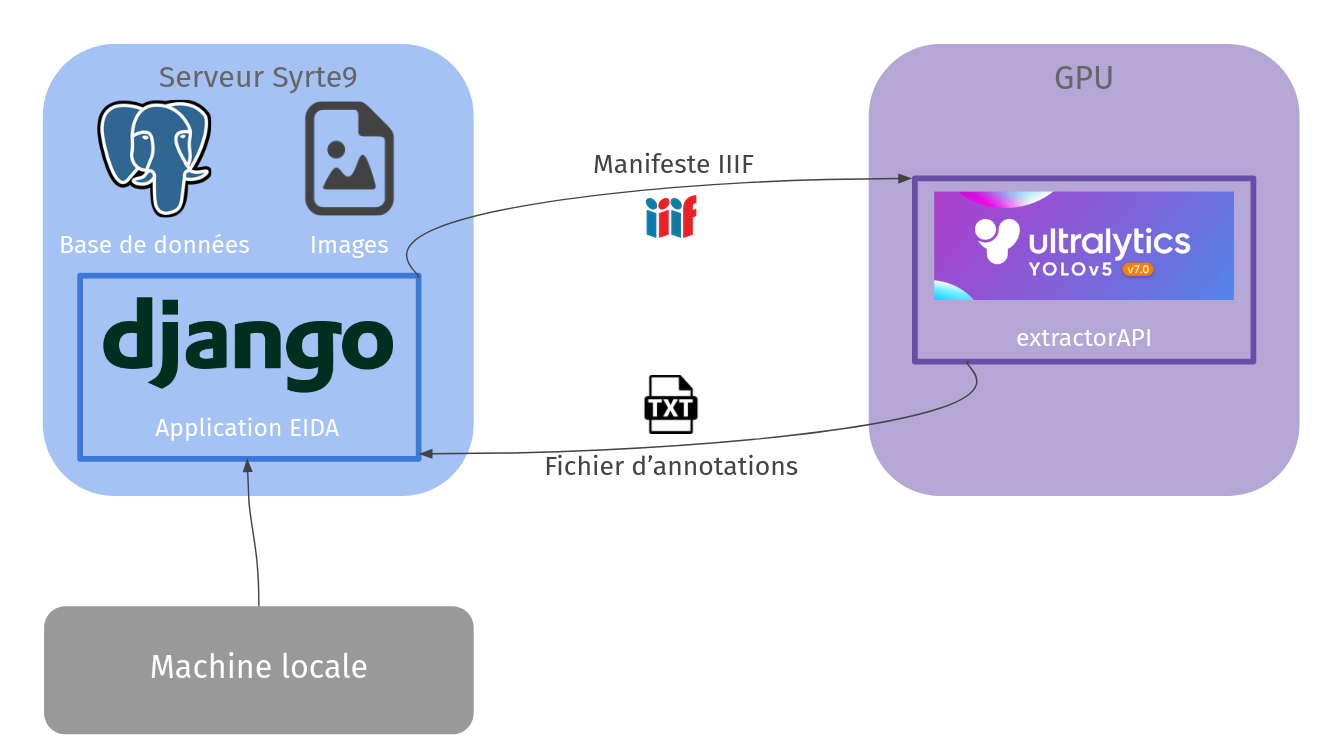
\includegraphics[width=15cm]{images/schema_archi.png}
		\caption{Schéma de l'architecture de l'application \eida et de l'\api \exapi}
		\label{fig:archi_eida}
	\end{figure}

\subsection{Cahier des charges et analyse des besoins}
    \subsubsection{Programmation modulaire et \textit{open source}}
    Avant le développement de l'\api, il est nécessaire d'établir les besoins auxquels cette dernière doit répondre par la rédaction d'un cahier des charges\footnote{Le cahier des charges pour le développement de l'\api a été réalisé lors du premier mois de stage.} (Annexe \ref{exapiCahier}), qui détaille les attentes techniques liées à l'outil créé. La création d'outils \textit{open source} réutilisables par d'autres projets étant un élément central du projet \eida, il est attendu de l'\api qu'elle réponde aux besoins spécifiques du projet tout en présentant la possibilité d'être réemployées dans d'autres contextes. Le lancement d'algorithmes de détection d'objets sur un \gpu est une tâche suffisamment généraliste pour être appliquée par d'autres projets de recherche utilisant la vision par ordinateur pour le traitement des sources historiques ; il est donc souhaitable de créer une \api réemployable pour éviter la multiplication d'outils similaires développés par des projets aux objectifs proches.
    
    Dans cette optique de libre accès, le code de l'\api est mis à disposition sur GitHub, avec la possibilité de le réemployer, en l'adaptant à l'architecture spécifique d'un projet et en modifiant simplement le modèle utilisé pour la détection. La création d'une \api indépendante de l'application \eida renforce la possibilité de remploi des outils développés, puisqu'en tant qu'entité séparée de l'application du projet, l'\api effectue des tâches peu spécifiques, et peut ainsi être intégrée à une application différente sans grandes modifications du code. 
    
    \subsubsection{API REST}
    La communication en \ssh entre le \gpu et l’application \eida n’étant pas satisfaisante du point de vue de la sécurité, le développement d’une \api permet de gérer ces échanges par une voie sécurisée. Il est défini dans le cahier des charges que l'\api communique avec l'application par le biais de requêtes \http qu'elle reçoit et envoie : en tant qu'interface pour la communication de l'application et du modèle de détection, l'\api reçoit des requêtes \http et retourne une ressource spécifique dépendant de l'\URL à laquelle la requête est envoyée.
    
    Par définition, l'\api développée est donc une \api \rest. \rest définit un ensemble de contraintes architecturales pour le développement de services web, qui permettent la communication et l'échange de données sur Internet. Les \api \rest sont basées sur des ressources localisées par des \URL\footcite{APIRESTEst} : lorsqu'un client demande une ressource, il envoie une requête \http\footnote{Les actions à effectuer sur la ressource sont définies par la requête \http : dans ce mémoire, nous mentionnons spécifiquement les requêtes GET, qui permettent au client de récupérer des données, et les requêtes POST, qui permettent d'envoyer des données avec la requête.} à un \textit{endpoint} de l'\api, qui retourne en réponse à cette requête une ressource dans un format standard\footnote{Le format \json, par exemple, est un format lisible et interprétable par les machines comme par les humains : il est le plus communément utilisé. \cite{APIRESTEst}}. Dans une \api \rest, les communications entre client et serveur sont \textit{stateless}, signifiant que les informations du client ne sont pas stockées entre les requêtes, et que les requêtes sont traitées indépendamment\footcite{APIRESTEst}. Les \api \rest reposent également sur une interface uniforme pour les interactions avec le client, et un système de couches qui assurent la flexibilité de l'\api et la sécurité des serveurs.
    
    Ainsi, une \api \rest permet la création de services web interopérables : elle facilite la communication entre différents systèmes informatiques en utilisant des requêtes \http pour accéder et manipuler des ressources. Ce mode d'échange des données étant standardisé, il est envisageable pour des projets futurs d'intégrer l'\api à leurs développements, à la seule condition que soit développée une application envoyant des requêtes en accord avec le protocole \http, apte à recevoir des requêtes de la part de l'\api. L'architecture \rest étant pensée pour l'uniformisation et l'intéropérabilité, un grand nombre d'applications sont construites autour de ces principes, et de nombreux \textit{frameworks} les prennent en compte dans les outils qu'ils proposent.
        
    \subsubsection{Sécurité et robustesse}
    Le cahier des charges rédigé en amont du développement de l'\api définit les contraintes du point de vue de la sécurité, des fonctionnalités souhaitées et des échanges de données. \exapi répond ainsi aux besoins spécifiques du projet et de l'application \eida, tout en en faisant le choix d'outils libres, standardisés, qui lui assurent d'être réutilisable dans des contextes et architectures variés.
    
    L'\api, déployée sur un \gpu mis à disposition de l'Observatoire de Paris, se doit d'être sécurisée, pour interdire les requêtes provenant de sources non-identifiées, et éviter ainsi un risque de surcharge de l'\api par des requêtes externes. Une authentification avec un token basée sur les principes \rest\footcite{grinbergRESTfulAuthenticationFlask} a été envisagée, ainsi qu'une restriction des hôtes autorisés à envoyer des requêtes aux \textit{endpoints} de l'\api.
    
    La question de la robustesse est également soulevée parmi les besoins fondamentaux en amont du développement : l'\api est une interface pour des algorithmes appliquant des traitements à des fichiers volumineux -- des images -- en grand nombre, et doit donc avoir la robustesse nécessaire pour accomplir ces tâches. En effet, l'\api reçoit des numérisations d'ouvrages sous la forme de manifestes \iiif, qui représentent ainsi plusieurs centaines d'images à enregistrer avant d'en extraire les objets. Les tâches de lecture du manifeste, d'extraction et d'enregistrement des images sont particulièrement chronophages, tout comme la détection d'objet, il est donc nécessaire de prévoir un gestionnaire de tâches, qui crée une file d'attente des requêtes reçues, afin que ces requêtes successives se lancent dans leur ordre de réception par l'\api, et que le traitement d'une nouvelle source ne se lance qu'après complétion du traitement de la source précédente. Le gestionnaire des tâches permet ainsi d'éviter la surcharge de l'\api en cas de requêtes simultanées, et assure son bon fonctionnement, un temps de traitement correct et une gestion cohérente des requêtes.
    
    Le mode de communication, la sécurité et la robustesse sont trois points fondamentaux du développement applicatif, qui représentent les attentes principales détaillées dans le cahier des charges pour le développement de l'\api. L'objectif d'\exapi est de proposer une structure flexible et légère pour l'inférence d'un modèle de vision artificielle sur un \gpu, afin d'extraire la détection d'objet de l'application du projet, pour en faire un module externe aisément modifiable, réutilisable, et adaptable à des modèles de détection, architectures et besoins variés.
	
\subsection{Développement de l'API}
	\subsubsection{Choix du \textit{framework} : Flask, Django ou FastAPI ?}
	Il existe divers \textit{frameworks}\footnote{Un \textit{framework}, littéralement \og cadre de travail \fg est une bibliothèque de composants logiciels ayant pour vocation à servir de base, ou de squelette, pour le développement d'une application dans un langage donné. Les \textit{frameworks} ont pour vocation de simplifier le travail des développeurs, tout en uniformisant les applications produites.} Python permettant le développement d'une \api. Ces \textit{frameworks} présentant tous des fonctionnalités spécifiques, la première étape du travail de développement d'\exapi est la sélection du \textit{framework} qui servira de squelette à l'application. Trois options ont été envisagées : Django\footcite{Django}, Flask\footcite{FlaskDocumentation} et FastAPI\footcite{FastAPI}.
	
	Django est un \textit{framework} développé en 2003 dédié au développement applicatif en Python, gratuit et en libre accès. L'application \eida, avec laquelle communique \exapi, est basée sur ce \textit{framework}, qui constitue ainsi une option logique dans la continuité du développement de l'application du projet. Les ressources en ligne pour l'intégration de PyTorch, module de \ml, à une application Django sont nombreuses\footcite{arslanCreateMachineLearning2021}, et il existe un \textit{framework} \rest\footcite{DjangoRESTFramework} qui simplifie le développement d'une \api à partir de Django. Apprécié pour sa robustesse, Django est cependant un \textit{framework} assez lourd, constitué de nombreux modules intégrés qui tendent à le ralentir\footcite{sandyChoosingDjangoFlask}. Django permet la création d'\api puissantes, avec des modules nombreux ; cependant, pour le développement d'une \api dont la priorité est la rapidité et la flexibilité, il existe des \textit{frameworks} plus légers, tels que Flask.
	
	Flask est un \textit{framework} pour le développement web en Python, basé sur un noyau simple dont les fonctionnalités peuvent être étendues. Minimaliste dans ses modules de base, les principes fondateurs de Flask sont la légèreté et la flexibilité, qui en font un \textit{framework} aisément adaptable à de nombreux projets, simple à prendre en main, et aux possibilités variées. \exapi ayant pour vocation d'être un module léger complémentaire à l'application \eida, il a été choisi d'utiliser Flask pour son développement, afin de produire une \api simple et flexible, qu'il serait aisé d'adapter à d'autres projets, ou aux étapes futures d'\eida, qui impliquent des modèles de vision artificielle aux objectifs différents des modèles de détection utilisés à ce stade.
	
	Le \textit{framework} FastAPI a également été envisagé pour le développement d'\exapi. Ce dernier ayant été publié en 2018, il intègre des fonctionnalités facilitant la rédaction de documentation\footcite{FastAPIFrameworkPython2023} pour l'\api développée, et est réputé pour sa rapidité\footcite{sandyChoosingDjangoFlask}. Sa flexibilité rendait ce \textit{framework} adapté au projet \eida et aux attentes entourant \exapi. Cependant, s'agissant d'un outil récent, la documentation comme la communauté ne sont pas aussi riches que pour les \textit{frameworks} précédemment mentionnés, il a donc été décidé de favoriser Flask pour ce projet, pour permettre un développement fluide et une mise à disposition rapide de l'\api.
	
	\subsubsection{Intégration du modèle de détection}
	L'application \eida et \exapi ayant, en premier lieu, pour vocation d'être des outils à la constitution de jeux de données d'entraînement et de vérité de terrain, il n'existe pas à ce jour de modèle de détection d'objet définitif à intégrer à l'\api. Dans son développement, il est donc nécessaire de prévoir la possibilité de choisir le modèle de détection utilisé, afin de substituer les modèles temporaires utilisés actuellement\footnote{Les modèles utilisés actuellement ne sont pas entraînés sur les données du projet, mais permettent de fournir aux chercheurs qui créent les données d'entraînement une première annotation imparfaite, qu'ils corrigent depuis l'interface d'annotation de l'application, accélérant le travail de création de cette vérité de terrain.} par un modèle entraîné lorsque l'étape d'entraînement sera complétée.
	
	Le script d’inférence utilisé est celui de \yolov\footnote{Il s'agit du script \texttt{detect.py} disponible en accès libre dans le dépôt GitHub du projet. \url{https://github.com/ultralytics/yolov5/blob/master/detect.py}}, reproduit et importé comme un module dans le code de l'\api, et appelé par une fonction lorsque le client envoie une requête à l'\textit{endpoint} servant à la détection d'objet. Le code de \yolov étant en accès libre, le script pour le lancement de la détection est réutilisé sans modification (Annexe \ref{yoloScript}), et comporte donc les options liées aux fichiers vidéo que \yolo propose initialement : la restriction des formats envoyés est gérée par l'application, qui ne supporte que les manifestes \iiif, les fichiers PDF et les fichiers image, qui sont transmis à l'\api sous forme de manifestes \iiif au format \json. Par défaut, le script fait appel à un modèle de détection \yolov générique, défini par le paramètre \texttt{weights} de la fonction \texttt{run\_vhs} : l'appel à un modèle personnalisé est défini dans les routes de \api\footnote{Les routes sont définies dans le fichier \texttt{app.py} : l'\api ne contenant que deux routes, une architecture simple a été choisie, et les routes ne sont donc pas dissociées du corps du code. \url{https://github.com/jnorindr/extractorAPI/blob/main/app.py}}.
	
	La route correspondant à l'\textit{endpoint} \texttt{/run\_detect} (fig. \ref{fig:run_detect_exapi})est utilisée pour soumettre une numérisation à traiter par le modèle : recevant de la part de l'application des requêtes \http POST contenant des données, celle-ci prévoit la réception de l'\URL d'un manifeste \iiif contenant les images à annoter, ainsi que le nom du fichier contenant le modèle à utiliser pour la détection. Elle permet ainsi, lors du paramétrage des échanges entre l'application et l'\api, de déterminer le modèle utilisé pour la détection d'objets.
	
	\begin{figure}[h]
		\begin{lstlisting}[language=Python]
		@app.route("/run_detect", methods=['POST'])
		def run_detect():
		# Get manifest URL from the request form
		manifest_url = request.form['manifest_url']
		model = request.form.get('model')
		
		# function.delay() is used to trigger function as celery task
		detect.delay(manifest_url, model)
		return f"Run detect task triggered with Celery! Check terminal to see the logs..."\end{lstlisting}
		\caption{Fonction de la route recevant des requêtes POST contenant une numérisation sur laquelle performer la détection d'objets}
		\label{fig:run_detect_exapi}
	\end{figure}

	La fonction \texttt{run\_detect()} fait appel à une fonction \texttt{detect()} de préparation au lancement de la détection, lancée en tâche de fond, dans laquelle la ligne de code suivante permet d'établir l'utilisation d'un modèle par défaut si aucun modèle spécifique n'est défini dans le formulaire envoyé à l'\textit{endpoint} par l'application (fig\ref{fig:model_exapi}).
	
	\begin{figure}[h]
		\begin{lstlisting}[language=Python]
		model = DEFAULT_MODEL if model is None else model\end{lstlisting}
		\caption{Fragment de code de la fonction \texttt{detect()}}
		\label{fig:model_exapi}
	\end{figure}

	Le modèle par défaut est défini dans le module d'utilitaires de l'\api\footnote{Parmi les utilitaires, le fichier \texttt{path.py} permet de définir les chemins dans l'application, et de les appeler en minimisant le risque d'erreurs. \url{https://github.com/jnorindr/extractorAPI/blob/main/utils/paths.py}}, et permet d'éviter une erreur si le modèle de détection n'est pas défini dans la requête envoyée par le client. La fonction \texttt{detect} fait ensuite appel à la fonction \texttt{run\_vhs}\footnote{Cette fonction correspond au script d'inférence de \yolov.} (fig. \ref{fig:run_vhs_exapi}), avec pour paramètres les informations envoyées dans le formulaire de la requête POST à l'\textit{endpoint} de détection, ainsi que les chemins des images sur enregistrées sur lesquelles performer la détection d'objets, et le chemin du fichier dans lequel doivent être écrites les annotations.
	
	\begin{figure}[h]
		\begin{lstlisting}[language=Python]
			run_vhs(
				weights=f"{MODEL_PATH}/{model}",
				source=wit_path / img,
				anno_file=anno_file,
				img_nb=i
			)\end{lstlisting}
		\caption{Fragment de code de la fonction \texttt{detect()} appelant la fonction \texttt{run\_vhs()} lançant la détection par le modèle}
		\label{fig:run_vhs_exapi}
	\end{figure}

	Ainsi, plusieurs modèles de vision artificielle peuvent être importés sur le \gpu, dans le dossier de l'\api, au format \texttt{.pt}\footnote{Le format \texttt{.pt} est un format standard pour les modèles de \ml créés avec PyTorch. \cite{dowlingGuideFileFormats2019}}. Ces modèles peuvent ensuite être appelés par le script dédié au lancement de l'inférence, avec des paramètres établis dans la requête envoyée par l'application \eida à l'\textit{endpoint} d'\exapi qui reçoit des numérisations pour leur traitement par l'algorithme de détection.

	\subsubsection{Formats des fichiers et échanges de données avec l'application}
	\exapi échange des données avec \eida dans des formats spécifiques, définis dès le cahier des charges, pour correspondre notamment aux exigences de formats pour l'entraînement d'un modèle. 
	
	L'\api reçoit de la part de l'application une requête POST contenant un manifeste \iiif, au format \json, qui permet d'échanger rapidement et de manière efficace des numérisations comportant un grand nombre d'images. Bien que les images de ces numérisations soient enregistrées dans l'application \eida après leur soumission par l'utilisateur, il n'est en effet pas envisageable d'envoyer par requête \http à l'\api un tel volume de fichiers image qui, en plus de représenter plus d'une centaine de fichiers par numérisation, sont des fichiers lourds. L'envoi de manifestes \iiif implique, après réception de la requête par l'\api, l'enregistrement des images sur le \gpu, qui constitue un traitement chronophage mais nécessaire pour la détection d'objets qui ne peut s'effectuer que sur des fichiers image enregistrés\footnote{Il est peu satisfaisant, en termes de performances et de gestion de la mémoire, d'enregistrer les images une première fois sur le serveur de l'application \eida, puis de les enregistrer une seconde fois sur le \gpu. Cependant, à ce jour, aucune chaîne de traitement ne nécessitant qu'un seul enregistrement des images ne s'est avérée satisfaisante -- des réflexions sont actuellement en cours pour modifier cette manière de procéder pour la rendre plus efficace.}. Pour plus d'efficacité, les images ne sont pas supprimées après l'étape de détection d'objet : celles-ci sont conservées pour permettre le lancement rapide de la détection en cas de nouvelle requête envoyée par le client pour une même numérisation. Cependant, le corpus traité par un projet tel qu'\eida représentant des plusieurs centaines -- ou plusieurs milliers -- de numérisations, il est nécessaire de prendre en compte la question de l'espace de stockage sur le \gpu utilisé pour la détection ; ainsi, une fonction avec une tâche périodique, planifiée avec \texttt{crontab}\footnote{\texttt{cron} est un programme permettant d'exécuter des tâches à une heure spécifique, selon un cycle spécifié à l'avance. \cite{Cron2023}}, supprime les images enregistrées sur le \gpu après une semaine.
	
	Après finalisation de la détection d'objets dans les images du document numérisé, \exapi retourne à l'application un fichier texte \texttt{.txt} contenant toutes les annotations, c'est-à-dire une liste des noms des fichiers image suivis des coordonnées des objets détectés. Un unique fichier d'annotation est généré pour chaque numérisation, et celui-ci contient les données pour chaque image de la numérisation. Le fichier d'annotation est envoyé à l'application \eida par une requête POST provenant de l'\api.
	
	\subsubsection{Gestion des tâches et files d'attente}
	\exapi a été conçue pour lancer sur le \gpu l'inférence d'un modèle de détection d'objets dans les images : l'\api est donc construite pour effectuer des tâches lourdes, requérant une grande puissance de calcul, qui ne peuvent être menées simultanément. \exapi a pour tâches le téléchargement de plusieurs centaines d'images extraites de manifestes \iiif, puis la détection d'objets dans ces images enregistrées : pour éviter sa surcharge, un gestionnaire de tâches robuste, permettant de paramétrer le nombre de requêtes traitées en parallèle, est nécessaire.
	
	Pour gérer la réception et le traitement des requêtes, qui peuvent arriver simultanément, alors qu'une tâche est déjà en cours, Celery\footcite{CeleryDistributedTask} a été implémenté dans l'\api, en tant que gestionnaire de file d'attente. Après création d'une instance Celery\footnote{La création de l'instance Celery fait appel à une classe \texttt{Celery} dont on définit en argument les modules ainsi que le \textit{back end} et le \textit{broker}, qui gère les messages. Cette instanciation suffit à l'implémentation de Celery dans une application : Celery est conçu pour permettre une prise en main facile, offrant une solution simple à des problèmes de gestion des files d'attente qui peuvent s'avérer complexes. \url{https://github.com/jnorindr/extractorAPI/blob/main/utils/celery_utils.py}}, les fonctions appelées en tâche de fond sont définies à l'aide d'un décorateur, puis sont appelées dans les fonctions des routes à l'aide de la méthode \texttt{.delay()} (fig. \ref{fig:celery_exapi}).
	
	\begin{figure}[h]
		\begin{subfigure}{1\linewidth}
			\begin{lstlisting}[language=Python]
			@celery.task
			def detect(manifest_url, model):\end{lstlisting}
			\subcaption{Décorateur pour définir la fonction \texttt{detect()} comme tâche Celery}
		\end{subfigure}
		\begin{subfigure}{1\linewidth}
			\begin{lstlisting}[language=Python]
			detect.delay(manifest_url, model)\end{lstlisting}
			\subcaption{Méthode pour le lancement de la fonction \texttt{detect()} en tâche Celery}
		\end{subfigure}
		\caption{Éléments nécessaires pour la définition et le lancement de la fonction \texttt{detect()} comme tâche Celery}
		\label{fig:celery_exapi}
	\end{figure}

	Ainsi, la lecture du manifeste \iiif, l'extraction des images et la détection d'objets sont définis en tant que tâches de fond gérées par Celery : il est ensuite possible, au lancement de l'application et de Celery, de définir un nombre de \textit{workers}, c'est-à-dire le nombre de tâches pouvant être menée simultanément. Si le nombre de requêtes reçues à un moment donné dépasse le nombre de \textit{workers} disponibles, une file d'attente se crée, et les requêtes en attente sont traitées après complétion des requêtes en cours. Celery permet ainsi d'éviter la surcharge de l'\api en cas de réception d'un grand nombre de requêtes, et d'assurer la gestion fluide des demandes de détection envoyées par les utilisateurs.
	Le développement d'une \api pour le lancement de l'inférence d'un modèle de \dl sur un \gpu doit ainsi se faire en prenant en considération les besoins techniques de la vision artificielle en termes d'espace de stockage, de robustesse et de puissance de calcul. Il s'agit en effet de traitements réalisés sur des images qu'il est nécessaire d'enregistrer, de stocker, de traiter, et de tâches de détection chronophages, qui répondent à des requêtes envoyées par le client -- l'application -- et doivent retourner une réponse en un temps satisfaisant. Ainsi, le développement d'\exapi se focalise en premier lieu sur la gestion des tâches et l'établissement d'une file d'attente pour éviter sa surcharge en cas de réception de nombreuses requêtes. Si une \api ne présente pas d'interface accessible aux utilisateurs, sa construction doit malgré tout se faire en prenant en compte leur expérience, ainsi, il est souhaitable de traiter les requêtes dans leur ordre d'arrivée, de manière cohérente, pour assurer une réponse sans temps d'attente prolongé. L'anticipation de la réception de nombreuses requêtes, des limites des capacités de stockage du \gpu ou des changements de modèle de détection permet d'assurer le développement d'un outil solide et flexible, réutilisable dans des contextes variés et adaptable à de nombreux projets aux ambitions diverses.
        	\\
        
        L'\textit{open source}\footnote{Le terme d'\textit{open source}, ou code source ouvert, désigne la pratique de mise à disposition du code source d'un logiciel sous licence libre, pour permettre gratuitement sa réutilisation, sa distribution et sa modification.} est une préoccupation centrale lors du développement d'outil pour les projets de recherche : il est en effet souhaitable de produire, dans la mesure du possible, des applications réutilisables par des projets futurs, pour assurer une continuité dans les travaux produits sans que se démultiplient les développements d'outils similaires. Ainsi, le remploi du code est au cœur des ambitions des équipes d'ingénierie : l'intégration de l'apprentissage profond à des projets d'histoire nécessite des outils spécifiques, construits autour de ces traitements des sources par l'\ia, qui restent néanmoins similaires -- ou comparables dans leurs besoins techniques -- d'un projet à l'autre. L'utilisation d'un \gpu pour la vision artificielle compte parmi les besoins matériels qui se traduisent entre les projets, ainsi, dans une optique de programmation modulaire, une \api externe à l'application \vhs/\eida a été développée pour répondre à ce besoin, sans être hautement spécifique aux besoins de ces projets comme pourrait l'être un module intégré à l'application. \exapi, l'\api développée dans ce cadre, est ainsi conçue, dès son cahier des charges, pour répondre aux besoins du projet \eida tout en restant réemployable dans d'autres contextes -- sont ainsi utilisés, pour sa construction, des outils libres qui en standardisent le développement, avec la vocation de produire une \api aussi flexible que robuste.
        \clearemptydoublepage
            
      	\chapter[\textit{Computer vision} et pratiques des chercheurs]{Intégrer la vision artificielle aux pratiques des chercheurs}
      	Le chapitre précédent établit, du point de vue du \textit{back end}, les besoins techniques pour l'intégration de la vision artificielle à une chaîne de traitement des sources historiques : ces préoccupations en termes d'architecture et de puissance de calcul sont celles des équipes d'ingénierie, et existent en parallèle des préoccupations qui concernent plus directement les utilisateurs, et impactent réellement les pratiques des chercheurs. Ce chapitre revient ainsi sur la chaîne de traitement des sources historiques dans sa totalité, depuis la numérisation fournie par l'utilisateur jusqu'aux résultats retournés pour le traitement par les chercheurs, et sur les échanges avec les utilisateurs, en termes d'interface mais également en termes de médiation.
               
            \section[\textit{Workflow} de traitement des sources]{De la numérisation à l’annotation : l'automatisation du traitement des sources}
                % De la numérisation à l’annotation : l'automatisation du traitement des sources

\subsection{Chaîne de traitement des sources historiques}
    \subsubsection{Du manuscrit aux diagrammes : construction d'une chaîne de traitement pour les sources astronomiques}
	Du point de vue de l'utilisateur, la détection d'objet dans une source numérisée représente une unique étape : après envoi d'une numérisation de manuscrit ou d'imprimé dans l'application, celle-ci est retournée après un délai accompagnée d'annotations qui signalent les illustrations détectées. Cette fluidité dans l'expérience de l'utilisateur repose sur une chaîne de traitement automatique qui prépare les sources pour leur affichage dans l'application et pour le lancement de la détection d'objet sur les images. Ces traitements, invisibles du point de vue de l'utilisateur, sont variés, allant de la transformation du format des fichiers soumis, à l'envoi de ces données à des outils externes, tels que des \api, pour leur traitement par des algorithmes de vision artificielle.
	
	Les traitements appliqués aux sources envoyées à l'application par les chercheurs du projet \eida est constituée de cinq grandes étapes (fig. \ref{fig:detection_workflow}), qui représentent elles-mêmes divers traitements appliqués au fichier soumis initialement, transformé à chaque étape. 
	
	\begin{figure}[h]
		\centering
		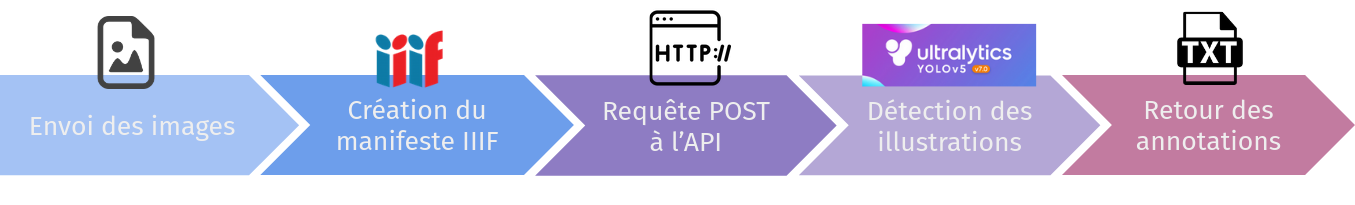
\includegraphics[width=16cm]{images/detection_workflow.png}
		\caption{Schéma de la chaîne de traitement du projet \eida pour la détection d'objet}
		\label{fig:detection_workflow}
	\end{figure}

	En premier lieu, depuis l'interface d'ajout d'un objet de l'application \eida (fig. \ref{fig:eida_list}), l'utilisateur remplit un formulaire de signalement du témoin avec un ensemble de métadonnées descriptives, et attache à ce formulaire une numérisation sous forme de manifeste \iiif, de fichier PDF ou d'un ensemble d'images aux formats \acrshort{jpeg} ou \acrshort{png}. Lorsque le formulaire est soumis, l'application retourne à l'utilisateur un message flash qui l'informe qu'un délai est nécessaire au traitement de la source, et que la numérisation annotée sera mise à disposition après finalisation de la détection. En parallèle, les images de la numérisation sont enregistrées : cette chaîne de traitement varie en fonction du format du fichier soumis par l'utilisateur\footnote{Les manifestes \iiif sont parsés pour en extraire les images, et les fichiers PDF sont fragmentés en une image par page et convertis en images au format PNG.}, et le résultat souhaité est l'enregistrement sur le serveur d'un fichier image par page de la numérisation.
	
	\begin{figure}[h]
		\centering
		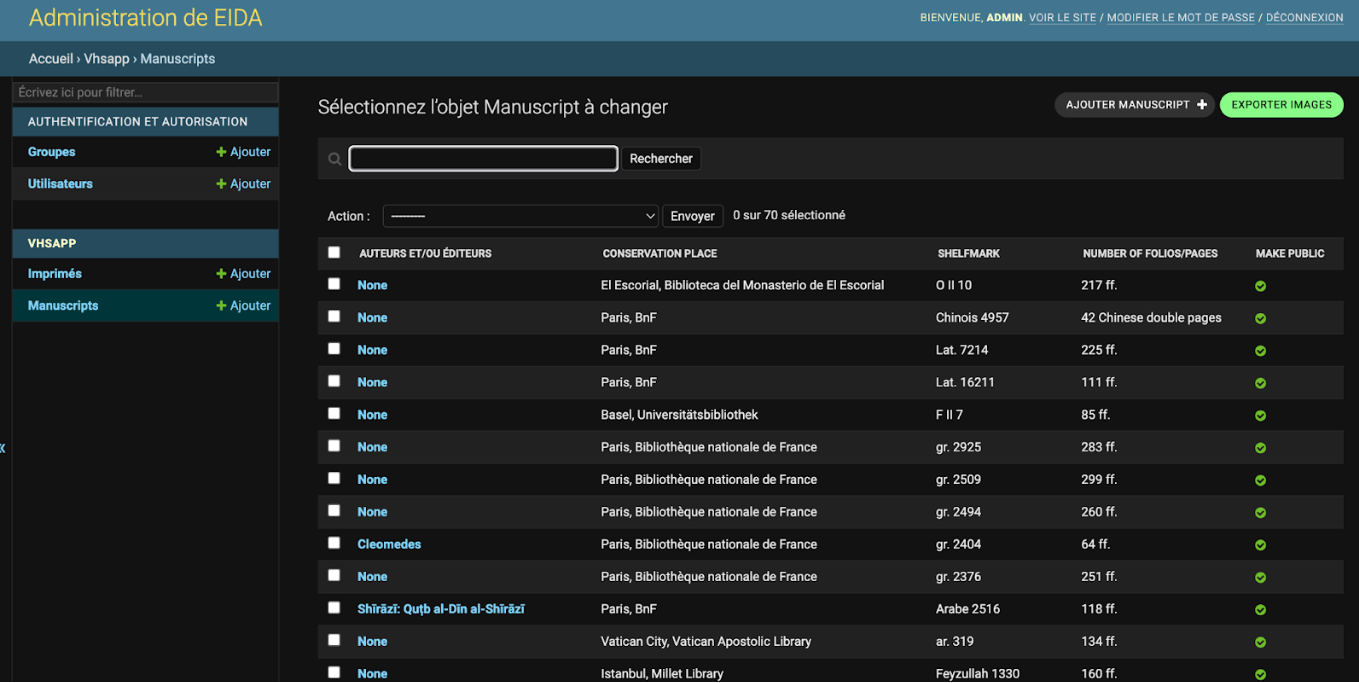
\includegraphics[width=16cm]{images/eida_list.png}
		\caption{Capture d'écran de l'interface listant les manuscrits saisis dans l'application \eida}
		\label{fig:eida_list}
	\end{figure}

	À partir des images de la numérisation enregistrées sur le serveur, un manifeste \iiif est généré par l'application\footnote{Comme mentionné dans la section \ref{stardardIiif}, malgré l'existence d'un standard, les manifestes \iiif présentent des disparités en fonction de leurs institutions d'origine. Pour assurer l'uniformité des manifestes utilisés pour la mise à disposition des sources du projet \eida, un nouveau manifeste est généré, y compris pour les numérisations déjà soumises sous la forme de manifestes \iiif.} : la numérisation est ainsi localisée par \URL, et peut être mise à disposition des utilisateurs selon un standard interopérable qui permet sa manipulation et sa réutilisation.
	
	Une fois le manifeste \iiif généré, une requête est envoyée à \exapi pour demander l'annotation des images par le modèle de détection. L'\URL du manifeste est envoyé par une requête \http POST : sa réception lance la chaîne de traitement des requêtes de l'\api, c'est-à-dire l'extraction et l'enregistrement des images à partir du manifeste \iiif, puis l'extraction des illustrations dans les images par le modèle de détection d'objet. 
	
	Après l'achèvement de la détection, le fichier d'annotations est retourné à l'application par une requête POST, et est enregistré sur le serveur. À partir de ce fichier texte, les détections sont indexées par le serveur \iiif d'annotation SimpleAnnotationServer\footcite{WelcomeSimpleAnnotation}, qui permet de lier les annotations avec les \textit{Canvases} correspondants dans une nouvelle version du manifeste \iiif du document étudié\footnote{Le manifeste \iiif de l'ouvrage existe donc en deux versions : une version \texttt{auto}, qui correspond à la numérisation sans annotations, et une version \texttt{v2}, à laquelle sont ajoutées les annotations.}. Cette indexation permet l'affichage des annotations sur l'image correspondante lorsque l'utilisateur consulte la numérisation dans un visualiseur \iiif.
	
	Le retour et l'indexation des annotations marque leur mise à disposition pour l'utilisateur : dans l'interface de modification des informations d'un témoin, un bouton permettant de visualiser les annotations apparaît (fig. \ref{fig:eida_buttons}), et permet de rediriger l'utlisateur vers une interface pour éditer manuellement les résultats de la détection automatique, et vers un visualiseur Mirador permettant de voir la numérisation accompagnée de ses annotations.	
	
	\begin{figure}[h]
		\centering
		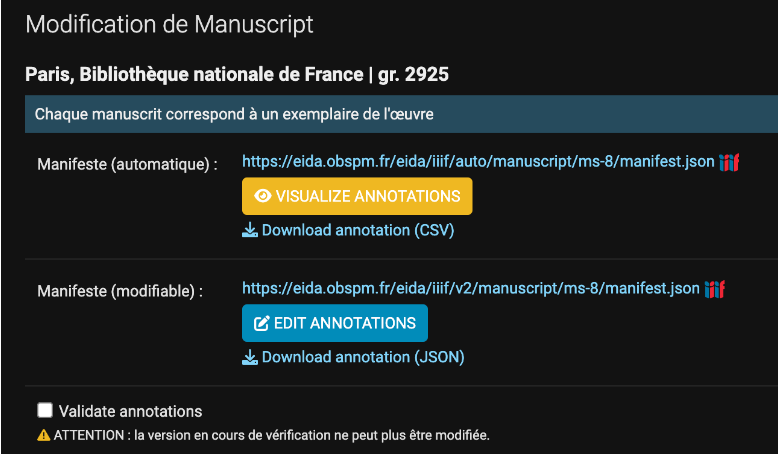
\includegraphics[width=12cm]{images/eida_buttons.png}
		\caption{Capture d'écran des boutons pour la visualisation du document numérisé et l'édition des annotations générées par le modèle de détection}
		\label{fig:eida_buttons}
	\end{figure}
	
	Ainsi, cette chaîne de traitement pour la détection automatique des objets dans les numérisations des sources remplace une recherche manuelle -- par les chercheurs -- des illustrations dans les ouvrages, permettant le traitement d'un corpus plus volumineux en un temps réduit. La détection ne représente cependant qu'une première étape pour le traitement des sources : elle est suivie d'interventions par les chercheurs, qui s'assurent notamment de la pertinence des traitements automatiques effectués.

    \subsubsection{Traitements automatiques, traitements manuels}
   	L'automatisation n'exclut pas un certain nombre d'actions manuelles sur les sources, et l'utilisation d'algorithmes de vision artificielle ne remplace pas le regard critique que peuvent porter les chercheurs sur les sources : il est donc nécessaire, dans les chaînes de traitement définies par les projets, de trouver un équilibre entre étapes automatiques et étapes manuelles de traitement des sources historiques, pour assurer, en finalité, des résultats les plus pertinents possibles.
   	
    Face à ce constat, il est nécessaire, pour les ingénieurs, de concevoir une chaîne de traitement qui va au-delà des étapes automatisées, et qui prend en compte la nécessité d'interventions manuelles entre chaque traitement pour un ajustement des résultats et une analyse primaire des données de sortie. Pour espérer produire des recherches aux résultats pertinents, il est ainsi nécessaire de savoir intégrer l'outil qu'est le \dl à un \textit{workflow}, et de trouver l'équilibre entre automatisation et tâches manuelles.
	
	La chaîne de traitement proposée par \eida propose ainsi une alternance d'étapes automatisées, en bleu sur le schéma, et d'étapes d'analyse par les chercheurs du projet, en violet (fig. \ref{fig:eida_workflow}).
    
    \begin{figure}[h]
    	\centering
    	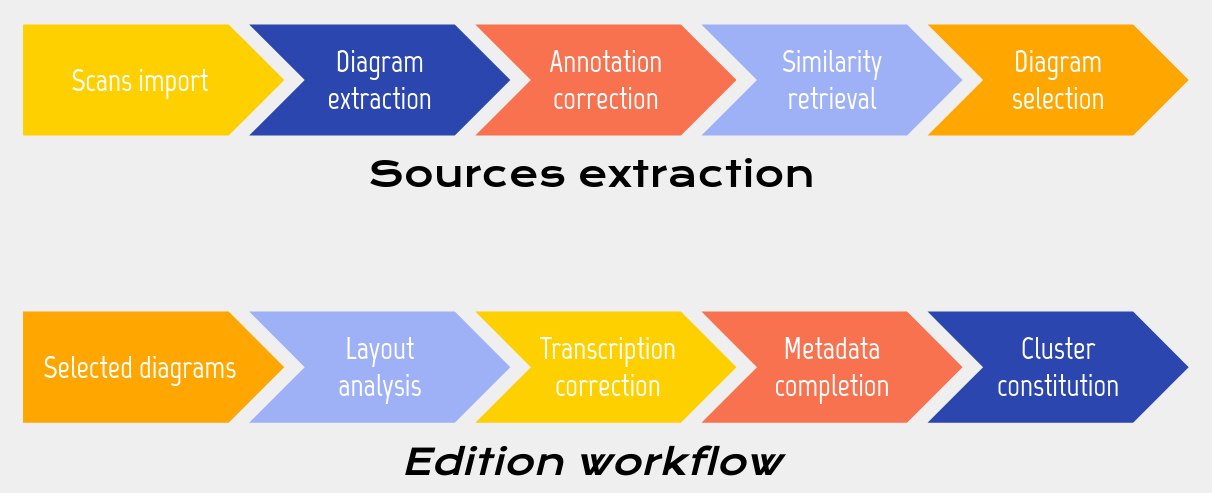
\includegraphics[width=16cm]{images/eida_workflow.png}
    	\caption{Schéma de la chaîne de traitement prévisionnelle des sources du projet \eida}
    	\label{fig:eida_workflow}
    \end{figure}

	Nous constatons ainsi que, suivant ce processus, l'\ia est employée comme un outil de pré-traitement des sources, permettant de naviguer un corpus volumineux et proposer une sélection de sources pour l'analyse par les chercheurs. Cette manière de procéder permet d'exploiter les forces des traitements par algorithmes de vision, et notamment la capacité à traiter un volume de données important en un temps très court. Pour la détection d'objet, la vision artificielle permet d'extraire automatiquement les illustrations d'un manuscrit en quelques minutes : les illustrations extraites devront toujours être corrigées par le chercheur\footnote{Comme expliqué dans le chapitre \ref{objectifsPossibilites}, il est nécessaire pour les performances de l'algorithme d'exclure ou d'inclure un certain nombre de cas limites lors de l'entraînement du modèle, ce qui donne en finalité un modèle de détection qui ne détecte pas nécessairement toutes les illustrations qui pourraient être jugées pertinentes par les chercheurs, ou qui détecte comme d'intérêt des illustrations sans rapport avec le projet de recherche.}, mais cette correction reste moins chronophage qu'une recherche manuelle des illustrations dans chaque source étudiée. L'alternance d'étapes manuelles et d'étapes automatiques permet d'assurer la pertinence des analyses produites, et de contrebalancer certains défauts -- tels que la binarité -- des algorithmes de \cv.
	
	Ainsi, les ingénieurs ont pour rôle -- en dialogue avec les équipes de recherche en histoire et les équipes de recherche en vision artificielle -- l'établissement d'une chaîne de traitement qui exploite les possibilités de la vision artificielle en prenant en compte ses limites. Le \textit{workflow} appliqué doit donc intégrer suffisamment d'étapes de correction manuelle pour produire, en finalité, des résultats pertinents, sans pour autant faire perdre son intérêt à l'usage d'algorithmes de \cv en nécessitant une trop grande intervention des chercheurs. Cet équilibre permet, en finalité, d'assurer la pertinence des données publiées par le projet de recherche, qui auront été étudiées par un prisme critique, tout en exploitant les avantages apportés par l'\ia en termes de volume des corpus traités.
	Ainsi, les ingénieurs ont pour rôle l'établissement d'une chaîne de traitement qui trouve un équilibre entre les possibilités et les limites de la vision artificielle. Le \textit{workflow} appliqué doit donc intégrer suffisamment d'étapes de correction manuelle pour produire, en finalité, des résultats pertinents, sans pour autant faire perdre son intérêt à l'usage d'algorithmes de \cv en nécessitant de trop nombreuses interventions des chercheurs. Cet équilibre permet ainsi, en finalité, d'assurer la pertinence des données produites par le projet de recherche, qui auront été analysées avec un regard critique que seuls les chercheurs peuvent apporter, et auront également bénéficié des avantages de l'\ia en termes de volume des corpus étudiés. 
	
\subsection{Annoter dans une interface graphique}
Pour permettre aux chercheurs des projets \eida et \vhs de corriger les annotations produites par l'algorithme de détection, une interface graphique est développée. En amont de l'entraînement du modèle de détection qui sera utilisé dans la version finale de l'application \eida, ces interfaces pour l'annotation ont pour objectif de fluidifier la constitution de vérités de terrain, c'est-à-dire la production d'un ensemble de numérisations annotées par les chercheurs qui serviront à l'entraînement et à la validation du modèle\footnote{Les données corrigées seront exportées par les ingénieurs des deux projets dans des formats correspondants à ceux attendus pour l'entraînement du modèle, c'est-à-dire images et texte brut.}.
 
Ces interfaces de correction des annotations, intégrées à l'application, rendent accessibles à l'utilisateur les résultats de la détection d'objet effectuée par le modèle de vision, par le biais d'une interface graphique qui lui permet de modifier ces données aisément. Après la mise en place d'un modèle entraîné et la publication de l'application, elles permettront aux chercheurs de corriger les annotations faites par le modèle pour en exploiter les résultats pour leurs travaux de recherche.

Les réflexions autour du développement de cette interface s'axent essentiellement autour de la praticité et d'une prise en main aisée, qui permet une correction rapide des résultats de la détection. Le projet \eida a ainsi fait le choix de deux interfaces liées, une première pour la suppression des objets détectés ne correspondant pas aux besoins du projet, et une seconde pour l'ajout d'objets manqués par le modèle et pour la modification des annotations non-conforme aux attentes. L'interface de suppression (fig. \ref{fig:eida_delete_anno})se présente sous la forme d'une liste d'images des pages de la numérisation, accompagnées d'images des objets détectés, qu'il est possible de supprimer en les sélectionnant puis en cliquant sur un bouton. Cette interface vise à proposer une vue d'ensemble de l'ouvrage numérisé sans nécessiter la consultation de la numérisation en parallèle, pour fluidifier la correction.
 	
 	\begin{figure}[h]
	\centering
	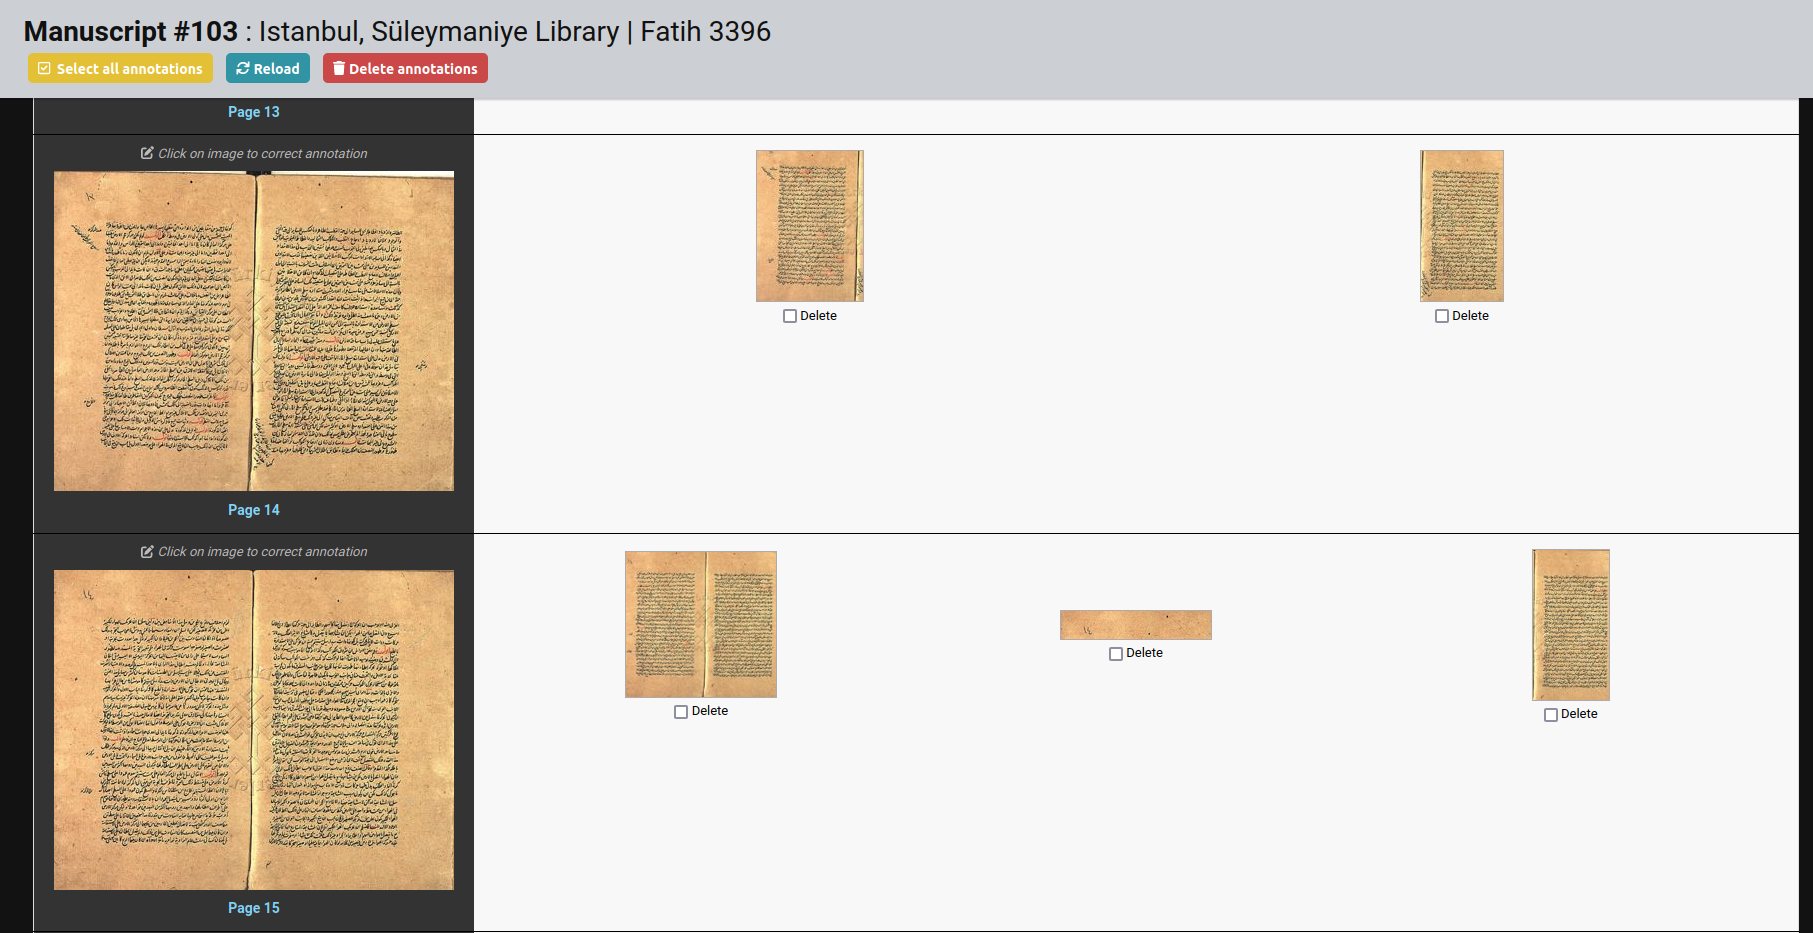
\includegraphics[width=16cm]{images/eida_delete_anno.png}
	\caption{Capture d'écran de l'interface \eida de suppression d'annotations}
	\label{fig:eida_delete_anno}
\end{figure}

Basée sur un visualiseur Mirador\footcite{MiradorHomea}, l'interface d'ajout et de modification des annotations exploite les possibilités offertes par le standard \iiif en intégrant à l'application \eida un outil \textit{open-source} apte à gérer les numérisations et leurs annotations, sans nécessiter de développement spécifique. Par cette interface, les chercheurs ont la possibilité d'ajouter des annotations ou de modifier le format des annotations déjà présentes, pour signaler des illustrations non-détectées ou adapter une détection fautives aux attentes du projet en termes d'annotations.

 	\begin{figure}[h]
	\centering
	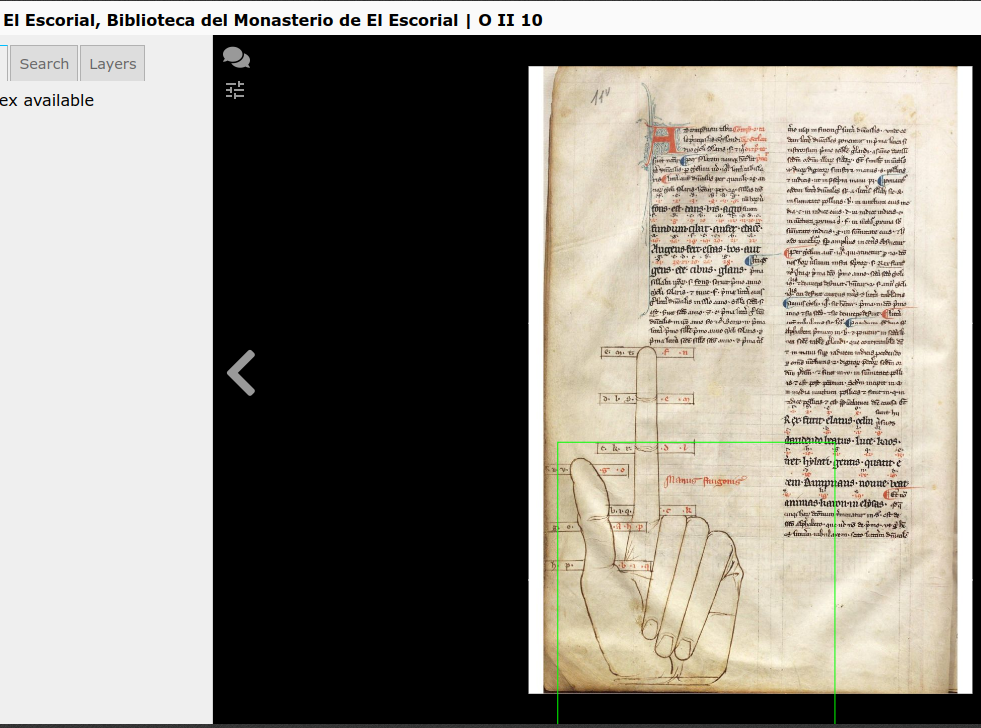
\includegraphics[width=14cm]{images/eida_add_anno.png}
	\caption{Capture d'écran du visualiseur Mirador \eida pour l'ajout et la modification des annotations}
	\label{fig:eida_add_anno}
\end{figure}

L'utilisation d'un visualiseur \iiif pour la gestion des annotations permet, pour les chercheur familiers avec le standard et ses outils, de prendre en main aisément cette interface de correction. Une documentation, rédigée par l'équipe d'ingénirie du projet \eida, est mise à disposition des chercheurs du projet pour la prise en main de ces interfaces : cette documentation permet d'assurer l'établissement d'une norme dans les choix effectués en termes de correction des données pour l'entraînement du modèle. Dans le futur, en prévision de la publication de l'application, une documentation destinée au grand public est à envisager, axée sur la prise en main des interfaces pour la correction de l'annotation par le modèle, sans l'enjeu de l'uniformisation des données pour l'entraînement. Une distinction est à faire entre les besoins actuels qui entourent ces interfaces, axés autour de l'entraînement de modèles de détection encore généralistes, et les besoins futurs, dans une application publiée et accessible à tous, où ces interfaces serviront à une correction en autonomie par les utilisateurs.

         
            \section{Médiation et documentation}
                % De la numérisation à l’annotation

\subsection{\textit{Workflow} d'annotation}
    \subsubsection{Sous-sous-section 1}
 La chaîne de traitement proposée par \eida (fig. \ref{fig:eida_workflow}) propose ainsi une alternance d'étapes automatisées, en bleu sur le schéma, et d'étapes d'analyse par les chercheurs du projet.

\begin{figure}[h]
	\centering
	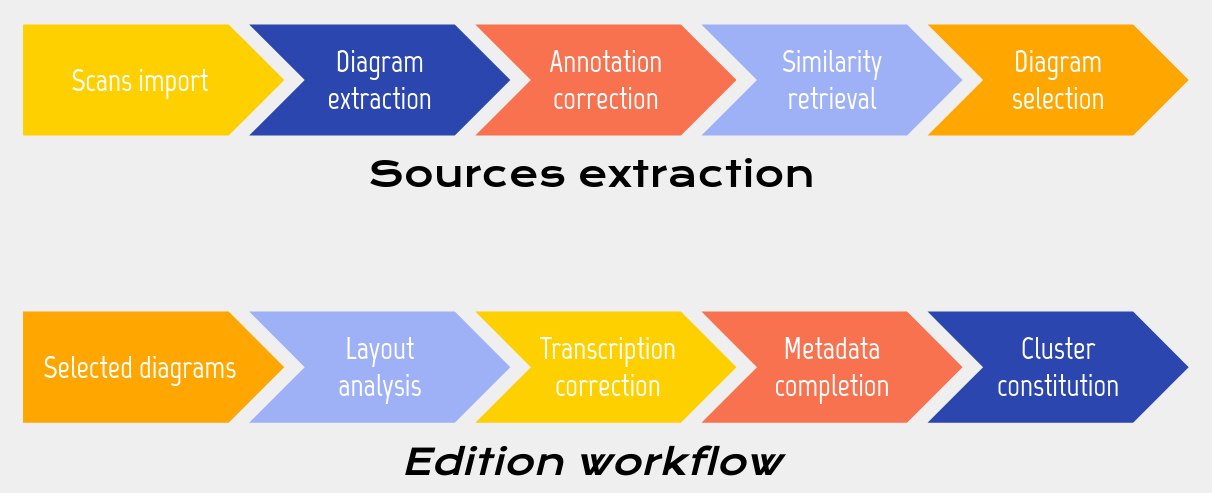
\includegraphics[width=15cm]{images/eida_workflow.png}
	\caption{\textit{Workflow} de traitement des sources du projet \eida}
	\label{fig:eida_workflow}
\end{figure}

    \subsubsection{Sous-sous-section 2}

    
    \subsection{Échanges et transformation des données}
        \subsubsection{Sous-sous-section 1}


        \subsubsection{Sous-sous-section 2}


    \subsection{Interface d’annotation}
        \subsubsection{Sous-sous-section 1}


        \subsubsection{Sous-sous-section 2}


        	\\
        
        L'intégration de la vision artificielle aux pratiques des chercheurs en humanités passe ainsi par l'établissement d'une chaîne de traitement qui trouve un équilibre entre besoins scientifiques et possibilités numériques, en mêlant étapes automatiques et correction manuelle pour s'assurer de la pertinence des données qui en découlent. L'automatisation n'est jamais totale : le traitement de sources historiques ne peut s'effectuer sans un regard critique, humain, qui contrebalance les limites de l'\ia qui ne permettent pas d'appréhender les objets étudiés sous tous les aspects nécessaires à prendre en compte dans le cadre d'une recherche historique. L'apprentissage profond et la vision artificielle s'insèrent donc dans les pratiques de chercheurs en histoire par le biais d'outils et d'interfaces qui appellent à leur contribution, à leurs corrections, et à leur regard sur les résultats produits par des algorithmes. Les ingénieurs ont pour rôle, dans ce contexte, de développer des outils et pratiques qui permettent ce lien entre les méthodes et techniques du \dl et les chercheurs en humanités, et d'établir une médiation fluide qui assure la pertinence du travail produit. Au-delà de la communication avec les chercheurs, utilisateurs des interfaces, il est du devoir des ingénieurs d'assurer la pérennité des outils créés par une documentation destinée à d'autres développeurs, pour permettre la maintenance du code, ou son réemploi dans des projets extérieurs : ces bonnes pratiques assurent ainsi la vie des développements produits, et leur bonne intégration dans un contexte de recherche plus large, en tant qu'outils libres pour le traitement des sources.
        \clearemptydoublepage

    \part{Perspectives pour le traitement des sources : vers un outil pour l’édition et la recherche}
        \chapter[Éditer des diagrammes]{Éditer des diagrammes : vectorisation et édition critique}
        La partie précédente s'attache à décrire l'intégration des techniques et méthodes de la vision artificielle aux pratiques des chercheurs, en s'appuyant notamment sur le développement d'outils pour l'utilisation d'algorithmes de détection d'objet. Tâche canonique de la vision artificielle, la détection d'objet dans les images est une pratique établie, dont l'intérêt pour la navigation des corpus est avéré par un nombre certain de projets récents, tels que CorDeep\footcite{CorDeep}, ayant produit et publié des applications intégrant des algorithmes de détection d'objet pour le traitement des sources.
        
        La vision artificielle est riche en possibilités : au-delà des outils de détection plus accessibles -- dont des modèles \textit{off-the-shelf} existent pour les projets qui souhaiteraient l'employer -- les traitements automatiques pour l'édition ou pour l'étude critique des sources sont considérés et étudiés. La détection d'objet n'est ainsi pas considérée comme une finalité, mais comme une première étape dans une chaîne de traitement qui intègre des étapes automatique de recherche de similarité, de \textit{clustering} ou de vectorisation\footnote{Par vectorisation, nous entendons la transcription de numérisations de diagrammes géométriques en images \svg.}, offrant de nouvelles perspectives dans le cadre de l'intégration de la vision artificielle à l'étude des sources. Pour des projets portés sur l'illustration scientifique, tels que le projet \eida, la vectorisation présente un intérêt particulier, ouvrant des possibilités en termes d'édition automatique des diagrammes.
        
            \section{Édition numérique des diagrammes astronomiques}
                % Édition critique numérique des diagrammes astronomiques

\subsection{Définir les pratiques de l'édition de diagrammes géométriques}
	Dans un article publié en 2010, Boris et Nicholas Jardin soulignent la disparité des pratiques d'édition des textes et des diagrammes dans l'édition critique de textes canoniques\footcite{jardineCriticalEditingEarlyModern2010}. Dans le domaine de l'histoire des sciences, où se pose particulièrement cette question de l'édition des diagrammes qui accompagnent le texte, les auteurs soulignent l'existence d'éditions critiques qualitatives de textes canoniques, dans lesquelles les diagrammes reproduits sont altérés pour correspondre au contenu du texte, délaissant ainsi la fidélité à la source historique. La critique de cette pratique émane essentiellement du constat suivant :
	
	\begin{displayquote}
		Ils ont effectués ces changements sans commentaire, une démarche qu'aucun d'entre eux n'aurait seulement envisagé de faire avec le texte [Traduction libre]\footnote{\textit{\og they had made those changes without comment, something none of them would have thought of doing with the text \fg}. \cite{jardineCriticalEditingEarlyModern2010}}.
	\end{displayquote}
    
    Pensés comme simple accompagnement des textes scientifiques, les diagrammes sont édités en tant qu'outil de compréhension du discours pour un lecteur contemporain, délaissant ainsi l'aspect historique et la richesse en termes de tradition des textes qu'ils peuvent porter. Face aux ressources lacunaires quant à la définition des pratiques d'édition des diagrammes, Jardine et Jardine soulèvent des problématiques assimilables à celles de l'édition critique des textes du point de vue de la gestion des erreurs et des variations, et de la modification des conventions au fil de l'histoire. 
    
    Ainsi, cette perception des diagrammes comme simple outil d'illustration du texte est remise en question, notamment dans les travaux d'Eastwood sur l'astronomie médiévale\footcite{eastwoodPlanetaryDiagramsRoman2004}, qui soulignent l'utilité des diagrammes comme support de compréhension, d'interprétation et de réinterprétation des textes, et argumente qu'une étude poussée des diagrammes présents dans les sources historiques permet une compréhension nouvelle des textes scientifiques : au-delà de simples illustrations, ils sont une clé d'analyse des idées et des théories scientifiques\footcite{jardineCriticalEditingEarlyModern2010}. En tant que nouvel objet d'étude, les diagrammes géométriques se placent comme élément d'intérêt pour l'établissement de la tradition d'un texte : dans un article publié en 2013, Dominique Raynaud souligne le fait que les erreurs présentes dans les diagrammes peuvent éventuellement \og faciliter la distinction et la hiérarchisation de manuscrits d'une même oeuvre [Traduction personnelle]\footnote{\textit{\og Therefore, diagrams make it easier to discriminate between and sort the manuscripts of a given work. \fg}\cite{raynaudBuildingStemmaCodicum2014}} \fg , renforçant cette idée de la nécessité d'éditions critiques qualitatives, qui rendent compte des erreurs et évolutions de ces représentations.
    
    L'édition critique des diagrammes est, pour l'historien, un enjeu scientifique récent, et les pratiques éditoriales dans ce domaine restent mouvantes, loin d'un cadre établit par une norme globale. De la reproduction stricte à la correction des erreurs, les choix de représentation des diagrammes appartiennent à l'éditeur : pour faire du diagramme un objet d'étude au même titre que le texte, ces derniers se doivent d'être considérés comme des sources historiques à part entière. L'ambivalence des besoins en termes de reproduction des diagrammes, de support de compréhension du texte à objet d'étude à part entière, rend complexes les choix binaires nécessaires à l'édition papier d'un texte. Dans ce contexte, l'édition numérique se présente comme une solution possible, qui redéfinit les limites de l'édition critique.
    
    \subsection{Édition critique numérique : pratiques, perspectives et limites}
        \subsubsection{Outils numériques pour l'édition critique}
		\begin{displayquote}
			Nous sommes certainement à l'aube de changements conséquents dans les pratiques éditoriales. De ce fait, il semble probable que la diffusion de l'édition numérique réduise la tension entre l'édition axée sur l'origine [des diagrammes] et celle axée sur la réception [Traduction personnelle]\footnote{\textit{\og 			We are surely on the verge of further very substantial shifts in editorial practice. Thus it seems likely that the spread of digital editions will reduce the tension between origin-focused and reception-focused editing. \fg}. \cite{jardineCriticalEditingEarlyModern2010}}.
		\end{displayquote}
	
		Boris et Nicholas Jardine soulignent, en conclusion de l'article précédemment cité, la transformation du paysage éditorial amorcée par la diffusion et la normalisation de l'édition numérique. Dans la continuité des questionnements liés à l'édition critique de diagrammes géométriques et aux limites de l'édition papier pour leur exploitation, le numérique se présente comme une solution potentielle aux choix tranchés que le support impose aux éditeurs. Jardine et Jardine envisage ainsi, sans mise en pratique, la possibilité d'éditions numériques qui rendent compte du rôle historique des illustrations dans la diffusion des idées et dans la pratique scientifique\footcite{jardineCriticalEditingEarlyModern2010}.
		
		En pratique, les solutions pour les éditions critiques numériques sont nombreuses, et présentent également leurs propres limites techniques, tout en étant parfois méconnues des chercheurs\footcite{apollonDigitalCriticalEditions2014} et appliquées sans uniformité entre les projets d'édition. L'enjeu, ainsi, porte également sur l'intégration des outils numériques aux pratiques de l'édition critique et de la philologie\footcite{apollonDigitalCriticalEditions2014}, et particulièrement dans le cadre de l'édition de diagrammes géométriques, qui se développe à l'origine dans un cadre peu défini. Les solutions appliquées, sans universalité, dépendent ainsi des compétences et pratiques des acteurs des projets, et les choix faits en termes d'outil varient profondément d'une édition à l'autre. Ainsi, si des initiatives diverses ont vu le jour pour la définition de normes et de standards pour l'édition numérique\footnote{Ces initiatives sont souvent axées sur le texte : nous pouvons notamment évoquer la \acrfull{tei}, standard basé sur le \acrshort{xml}, qui vise à définir une norme pour la représentation numérique du texte par la publication de guides d'encodage.}, les projets restent libres dans leur procédé éditorial\footcite{apollonDigitalCriticalEditions2014}.
		
		Dans ce contexte, et face à l'existence d'un grand nombre d'outils pour l'édition critique du texte, il n'existe pas de normes numériques pour l'édition des diagrammes géométriques\footnote{Dans ce contexte, nous employons le terme d'édition pour décrire la transformation d'un diagramme existant au format papier -- ou en tant qu'image numérique d'une source -- en objet informatique manipulable pour l'analyse, la publication, ou l'édition numérique.}, et leur transformation en objets informatiques s'appuie souvent sur l'adaptation d'outils et de pratiques dédiés aux textes et réadaptés à ces sources visuelles. À titre d'exemple, l'Académie des Sciences de Berlin-Brandenburg mène depuis 1919 un projet -- toujours en cours -- d'édition critique monumentale de l'œuvre de Gottfried Wilhelm Leibniz. En 2009, l'édition prend un tournant digital sous la forme du projet Leibniz-Online\footcite{LeibnizOnlineLeibnizEditionc}, qui a fait le choix du langage \LaTeX en tant qu'outil pour l'édition numérique. \LaTeX étant un outil dédié à la mise en forme de documents, les fonctionnalités adaptées à l'édition critique de textes sont nombreuses ; pour les diagrammes, nombreux dans les textes de Leibniz et transcrits à partir des diagrammes manuscrits présents dans les sources primaires, Leibniz-Online fait le choix d'une exécution en \LaTeX également, en adaptant des \textit{packages} existant pour la création de schéma (fig. \ref{fig:leibniz_diag}). Les diagrammes transcrits sont rendus disponibles au format PDF dans un dépôt GitHub contenant le code de l'édition\footcite{LeibnizVIIILaTeX_TEIa}, et existent ainsi en tant qu'objets informatiques dans un format peu manipulable, figé après compilation. La transcription en \LaTeX de ces diagrammes est une étape manuelle effectuée par les éditeurs du projets, et représente une tâche particulièrement chronophage du processus d'édition\footnote{Ces explications sont basées sur une présentation donnée par l'équipe du projet Leibniz-Online à l'occasion d'une rencontre organisée par le projet ERC Adg PHILIUMM (laboratoire SPHERE) à l'Université de Paris.}. Les diagrammes encodés en \LaTeX emploient de nouvelles commandes créées pour les besoins spécifiques d'une édition, qui ne s'alignent donc sur aucun standard qui en assurerait l'intéropérabilité. Le projet d'édition critique de l'œuvre de Leibniz est, à ce jour, en cours depuis plus de cent ans : il se pose ainsi la question de la pérennité du code et de la transmission des pratiques de transcription. 
		
		\begin{figure}[h]
			\centering
			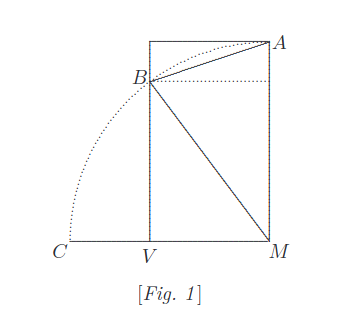
\includegraphics[width=15cm]{images/leibniz_diag.png}
			\caption{Diagrammes extraits de l'édition numérique de l'œuvre complet de Leibniz, volume VIII, 3, p. 665}
			\label{fig:leibniz_diag}
		\end{figure}
	
		En l'absence de norme pour l'édition numérique des diagrammes, les projets ont la liberté de sélectionner les outils, méthodes et formats employés, créant ainsi un paysage disparate de la transcription des diagrammes géométriques, sans pratiques communes et uniformes entre les différents projets. La transcription de ces diagrammes sous forme d'objets informatiques en vue de leur édition est souvent une étape chronophage, manuelle, faisant appel à des outils qu'il est nécessaire pour les chercheurs de prendre en main\footnote{On peut citer, à titre d'exemple, le logiciel libre GeoGebra qui, s'il n'est pas destiné à l'édition, permet la création de diagrammes numériques dans des formats divers. \cite{GeoGebra}}.
		
		Face à cette absence de solution numériques uniformes pour la transcription des diagrammes géométriques, l'\ia intervient comme une solution à la copie manuelle de diagrammes pour leur transformation en objet informatique depuis la source primaire. L'application à l'édition de diagrammes d'algorithmes de vectorisation permet de considérer une automatisation de chaînes de traitement à ce jour essentiellement manuelle, et de penser le développement d'outils libres destinés à l'édition qui définiraient des pratiques systématiques pour la création de versions numériques de diagrammes géométriques.

        \subsubsection{Définition des pratiques pour les diagrammes astronomiques}
        L'existence d'une interface numérique pour l'analyse de diagrammes présente un nombre d'avantages face à leur édition papier, limitée d'un point de vue matériel, et forçant l'éditeur à des choix qui ne correspondent pas nécessairement aux besoins d'un projet de recherche. Les versions numérisées de diagrammes géométriques permettent des actions pour l'analyse qui transcendent les limites physiques des sources historiques : il est ainsi possible d'envisager une comparaison de diagrammes par superposition, qui permettrait de souligner les évolutions d'un même diagramme dans les différentes versions d'une œuvre, d'enrichir les transcriptions de métadonnées pour en expliciter les éléments et choix éditoriaux, ou de faciliter la fouille de corpus de diagrammes, de leur appliquer des manipulations diverses, et de proposer une assistance à l'édition numérique des éléments visuels de textes scientifiques. Ces perspectives rendent cruciale la création d'interfaces pour l'étude et le traitement des diagrammes, à l'image des possibilités, outils et méthodes existants pour l'édition numérique du texte.
        
        Le projet \eida a pour ambition de créer une plateforme destinée à l'édition des diagrammes astronomiques, intégrant la vision artificielle pour proposer des fonctionnalités de transcription automatique. En amont du développement des plateformes et de l'entraînement d'algorithmes de vectorisation, la question des modalités d'édition des diagrammes se pose -- en lien avec les chercheurs, toujours dans une optique de répondre à leurs besoins et de produire des plateformes qui serviront leurs travaux -- pour définir les pratiques qui influenceront la création des outils. Trois types d'édition, c'est-à-dire de transcription à partir d'une image scannée d'un diagramme, sont envisagés : l'édition diplomatique, qui reproduit fidèlement le diagramme sur l'image en incluant ses erreurs, l'édition recalculée, qui prend en compte des paramètres encore à définir pour produire une version corrigée du diagramme, ou une édition critique, qui met en parallèle différentes versions d'un même diagramme pour en souligner les différences. Ces trois types d'éditions présentent un intérêt dans le cadre des recherches effectuées sur ces sources historiques, de l'étude de la circulation des idées à l'analyse de la pratique scientifique dans un contexte historique donné. L'emploi d'algorithmes de vision artificielle permet, à ce jour, de trancher en faveur d'une édition diplomatique, qui transcrirait à l'identique le diagramme soumis. La vectorisation sans correction est, en effet, ce que permet à ce jour la technique ; ainsi, comme mentionné dans les chapitres précédents, il est nécessaire de trouver un équilibre entre les attentes des chercheurs et les possibilités de ce type d'algorithme de vision.

        
            \section[De l’image aux vecteurs]{\label{vectorEdition}De l’image aux vecteurs : la vision artificielle pour l’édition numérique}
                % De l’image aux vecteurs : la vision artificielle pour l’édition numérique

\subsection{Automatiser la transcription}
    \subsubsection{Sous-sous-section 1}

    
    \subsubsection{Sous-sous-section 2}

    
    \subsection{Données d’entraînement et annotations pour la vectorisation}
        \subsubsection{Sous-sous-section 1}


        \subsubsection{Sous-sous-section 2}


    \subsection{Diagrammes en SVG}
        \subsubsection{Sous-sous-section 1}


        \subsubsection{Sous-sous-section 2}


        	\\
        
        La vectorisation automatique de diagrammes géométriques ouvre de nombreuses perspectives en termes de soutien à la recherche, et permet d'envisager des outils et interfaces à destination des chercheurs qui proposeraient d'automatiser des tâches autrement chronophage. La transcription des diagrammes, en lien avec l'histoire récente de l'édition critique de ce type d'illustration, fait l'objet d'un nombre restreint -- si ce n'est inexistant -- de normes qui en encadrent la pratique : les méthodes appliquées pour la transcription et l'édition numérique sont donc variées, spécifiques aux projets qui les emploient, et les objets informatiques générés ne sont pas nécessairement manipulables ou interopérables. Le \svg, format libre, est particulièrement appropriés pour l'étude des diagrammes : la transformation d'une numérisation en objet vectoriel devient alors une étape clé de la chaîne de traitement. Manuellement, cette dernière demande la connaissance d'outils spécifiques pour cette pratique. Ainsi, l'intégration à cette chaîne de traitement d'algorithmes de \cv est une opportunité de définition de normes et de pratiques pour la transcription, tout en rendant envisageable le traitement d'un volume important d'images en un temps moindre. La création d'outils libres, accessibles et aisés à prendre en main intégrant ces méthodes a vocation à faciliter cette étape chronophage du processus d'édition, et de permettre une analyse des diagrammes tirant réellement parti des avantages du numérique.    
        \clearemptydoublepage
        
        \chapter[\textit{Similarity retrieval} et \textit{clustering}]{Recherche de similarité et partitionnement de données}
        Le partitionnement de données (\textit{clustering}) et la recherche de similarité (\textit{similarity retrieval}) sont des tâches de vision artificielle dont l'application a déjà fait ses preuves. Particulièrement recherchées dans le domaine commercial, pour proposer notamment des recommandations aux utilisateurs en fonction de leurs intérêts\footcite{gronneIntroductionEmbeddingClustering2022}, elles permettent -- par des méthodes profondément différentes -- de regrouper des données en groupes cohérents. Pour le traitement d'images de sources historiques, le \textit{clustering} permet d'identifier des ensembles de sources présentant des aspects communs. La recherche de similarité permet, à partir d'une illustration donnée, d'identifier des copies plus ou moins fidèles, ou le réemploi de certains motifs. Ces deux méthodes s'appuient sur un fonctionnement similaire, qui transforme les images en valeurs numériques\footnote{On parle alors d'\textit{embedding}.} et en détermine les coordonnées dans un espace de grande dimension (\textit{high dimensional space})\footnote{Dont les caractéristiques sont définies en amont par extraction à l'aide d'un réseau de neurones artificiels. \cite{moiraghiExplorerCorpusImages2018}}, pour les y placer sous forme de point. Le \textit{clustering} identifie dans cet espace les points proches, et les réunit dans un nombre approprié de groupes\footcite{gronneIntroductionEmbeddingClustering2022}. La recherche de similarité se base sur la transformation des images d'entrée en vecteurs placés dans un espace de grande dimension\footnote{ Il est également possible de considérer pour chaque image un unique point placé dans l'espace de grande dimension : la requête de recherche de similarité retournera alors les points les plus proches, classés par proximité. \cite{dilenardoVisualPatternsDiscovery}} pour en calculer la similarité\footnote{Il existe plusieurs méthodes pour calculer la similarité de deux vecteurs, basées sur la distance euclidienne ou sur le cosinus de l'angle formé par ces vecteurs. \cite{gronneIntroductionEmbeddingClustering2022}}. Les perspectives ouvertes par ces algorithmes en termes d'outils pour la recherche sont nombreuses, et permettent d'envisager l'exploration de corpus volumineux par comparaison ou regroupement des sources, pour discerner dans les données des motifs et rapprochements autrement invisibles.
        
            \section[La recherche de similarité]{La recherche de similarité pour l'étude de la circulation des images}
				% Le clustering comme outil pour les chercheurs

\subsection{Sous-section 1}
    \subsubsection{Sous-sous-section 1}


    \subsubsection{Sous-sous-section 2}

    
    \subsection{Sous-section 2}
        \subsubsection{Sous-sous-section 1}


        \subsubsection{Sous-sous-section 2}

       		\section[Le partitionnement de données]{Le partitionnement de données : découvrir des motifs dans un corpus}
       			% Le clustering comme outil pour les chercheurs

\subsection{Sous-section 1}
    \subsubsection{Sous-sous-section 1}


    \subsubsection{Sous-sous-section 2}

    
    \subsection{Sous-section 2}
        \subsubsection{Sous-sous-section 1}


        \subsubsection{Sous-sous-section 2}
        	\\
        
        L'emploi de méthodes de vision artificielle pour des tâches de partition des données et de recherche de similarité permet d'envisager une automatisation du traitement des documents historiques qui inclut des outils pour une première analyse des sources, en proposant un regard global sur les données, qui donne ensuite lieu à une étude critique par les chercheurs. Les récentes avances techniques dans ces champs spécifiques produisent ainsi des résultats prometteurs pour le traitement d'objets historiques, qui permettent de véritablement les considérer dans un contexte applicatif à destination des chercheurs en humanités. Si la communication sur les possibilités réelles de l'\ia est toujours nécessaire pour tempérer les attentes scientifiques autour des algorithmes, un \textit{workflow} équilibré entre exploitation des forces de la \cv et traitement manuel pour la correction, l'annotation et l'analyse des résultats permet de concevoir des outils ouvrant des perspectives diverses, nombreuses, en termes de manipulation et d'étude des sources. La mise à disposition de ces techniques pour un public d'historiens permet d'envisager une création aisée d'objets numériques répondant aux besoins éditoriaux des chercheurs, pour la publication des résultats des projets de recherche et pour la navigation des données sur des plateformes ouvertes, accessibles, navigables. 
        \clearemptydoublepage
    
    \chapterNo{Conclusion}
    \addcontentsline{toc}{chapter}{Conclusion}
	L'intégration de méthodes et techniques de vision artificielle au traitement des sources historiques redéfinit fondamentalement le travail des chercheurs sur les documents, et offre en termes de recherche en humanités des perspectives nombreuses par un nouveau regard sur les sources et une appréhension différente de leur contenu.
	
	En amont des traitements par des algorithmes de vision, nous avons évoqué la question des données, de leur forme, depuis la constitution d'un corpus jusqu'à l'objet numérique support des tâches de vision. L'automatisation permet de considérer des corpus de recherche au volume important, puisqu'elle permet la navigation d'ensembles massifs de données en un temps réduit. Ainsi, les corpus établis par les projets mentionnés dans ce mémoire constituent des ensembles aux bornes chronologiques, géographiques et thématiques vastes, permettant des études globales, transversales, des sources, avec un intérêt particulier pour la tradition, la transmission, la copie et la circulation. La vision artificielle rend possible ces études aux cadres vastes en automatisant les tâches de collation et de transcription, qui par leur aspect chronophage interdisent l'étude manuelle d'un volume important de sources dans des projets au temps et aux ressources limitées. Par ces aspects, l'\ia appliquée à la recherche historique redéfinit les possibilités en termes de sujets étudiés et de regard qu'il est possible de porter aux sources, avec un accent mis sur les recherches transversales permises par les traitements automatiques, qui permettent, par exemple, de dessiner des liens insoupçonnés entre des sources provenant de contextes divers, et ainsi d'ouvrir des pistes d'analyse et de réflexion.
	
	Les traitements automatiques appliqués aux sources impliquent des étapes préliminaires de numérisation, de publication et de modélisation des données, qui possèdent leurs propres enjeux. Ce mémoire revient ainsi sur l'existence numérique des images, depuis leur numérisation -- qui représente en elle-même une tâche complexe, hors du cadre des projets de recherche -- jusqu'à leur mise en ligne. La numérisation des sources historiques définit, en amont de toutes les tâches décrites dans ce mémoire, la faisabilité des projets de recherche, et particulièrement dans un contexte d'inclusion de méthodes d'\ia. Pour la construction des corpus massifs précédemment évoqués, la disponibilité d'ensembles larges de numérisations est essentielle. Au-delà de la numérisation, la question de la mise à disposition et du partage des images est un enjeu d'interopérabilité, au service de la science ouverte, que des standards tels que \iiif visent à fluidifier et faciliter, pour renforcer le lien entre les institutions et les projets, et élargir les possibilités en termes de manipulation et de réutilisation des images.
	\\
	
	Le présent mémoire reconstitue la chaîne de traitement des sources historiques prévue par le projet \eida, intégrée à une application dont le développement est, à ce jour, toujours en cours. Les techniques abordées sont donc celles entrevues dans le cadre du projet, et ne rendent pas compte de la diversité des possibilités offertes par la vision artificielle pour la résolution d'autres tâches, telles que la classification\footcite{shenLargeScaleHistoricalWatermark2019}, la détection de poses, ou la transcription de texte et d'écritures, qui ont fait leurs preuves dans des contextes divers, des institutions patrimoniales aux projets de recherche en humanités. La vision artificielle, loin d'être monolithique, propose ainsi un ensemble de solutions à des tâches variées, qui peuvent être envisagées pour répondre à des besoins divers, de la navigation et l'organisation de collections numériques à l'analyse d'éléments spécifiques d'œuvres d'art.
	
	L'utilisation de techniques de vision artificielle pour le traitement des sources nécessite une médiation claire entre les chercheurs en humanités et les chercheurs en vision artificielle : ce rôle de médiation, tenu notamment par les ingénieurs des projets, mène à l'établissement d'un ensemble de normes qui créent un équilibre entre les attentes scientifiques des historiens et les possibilités techniques de la \cv. Les tâches effectuées par des algorithmes de vision présentent des limites, posées notamment par la binarité des modèles qui n'apportent pas de regard critique sur les sources, et qui nécessitent donc une définition claire et rigoureuse des résultats attendus. Ces attentes constituent un compromis, et les prédictions effectuées doivent faire l'objet d'une analyse et d'une correction systématiques par les chercheurs pour s'assurer de la pertinence des données produites, et pour compléter les résultats automatiques d'une analyse scientifique. La vision artificielle -- qu'il s'agisse de détection d'objets, de \textit{clustering}, de vectorisation ou de recherche de similarité -- doit ainsi être perçue comme un outil pour des tâches spécifiques d'une chaîne de traitement qui inclut des interventions manuelles sur les données d'entrée et de sortie. Les performances des modèles évoqués dans ce mémoire dépendent de la qualité des données annotées, corrigées, fournies pour l'entraînement ou pour la validation, qui permettent de calibrer les modèles pour permettre des prédictions précises, réellement exploitables pour la recherche en humanités.
	
	L'établissement d'une chaîne de traitement automatique des sources passe par le développement d'applications et d'interfaces, pour en faire un outil véritablement exploitable par un public de chercheurs. Ce mémoire explicite ainsi les développements en cours et prévus du projet \eida, et particulièrement la construction de fonctionnalités intégrées à l'application destinée aux chercheurs du projet. En prenant en compte les besoins scientifiques, les développements produits ont pour objectif de faire le lien entre les modèles de \cv et les utilisateurs, en proposant des interfaces faciles à prendre en main, qui permettent la réalisation de tâches manuelles de correction et d'annotation des images, en prévision de la publication de l'application pour un usage libre des outils produits. Dans un contexte d'émulation autour de la vision artificielle dans la recherche en humanité, les outils sont développés avec la volonté d'une mise à disposition du code pour leur réutilisation : un ensemble de bonnes pratiques a donc été établi, notamment en termes de médiation autour des développements, pour les chercheurs comme pour les développeurs qui souhaiteraient les réemployer.
	
	Ainsi, les perspectives ouvertes par les techniques de vision artificielle sont nombreuses, et font appel à une redéfinition des méthodologies de la recherche qui passent par la construction de plateformes dédiées, vectrices d'échanges entre les chercheurs en humanités et les chercheurs en \ia. La construction de modèles et de méthodes pour effectuer des tâches variées donne à ce jour des résultats prometteurs qui, malgré leurs limites, présagent un nouveau regard sur les sources historiques par l'angle de l'automatisation. Dans ce cadre, l'équilibre entre les attentes scientifiques et les possibilités techniques est une notion essentielle, au cœur des projets présentés dans ce mémoire, et constitue le socle d'une intégration pertinente de la \cv au traitement des sources historiques.
    \clearemptydoublepage
    
\appendix
    \part*{Annexes}	
    \addcontentsline{toc}{part}{Annexes}
    
    \chapter[Prepare custom data for training]{\label{YOLOv5Training}Prepare custom data for training using the YOLOv5 workflow}
	    \section{What is \yolov?}
	\begin{itemize}
		\item Built to detect objects in images
		\item Trained with a dataset of real images (ImageNet)
		\item Default model based on 80 object classes
	\end{itemize}

The goal of the training is to \textbf{adapt the model} to \textbf{our images and our classes}, for it to detect the objects we want it to.

\section{Training dataset}
	\begin{itemize}
		\item \textbf{Annotate the objects} of interest on the images to \textbf{create labels} : the objects are defined by the \textbf{position and dimensions of the rectangular box} surrounding them;
		\item The label file is a \texttt{.txt} file;
		\item In the label file, each object corresponds to \textbf{one row}: \texttt{class x\_center y\_center width height}
		\item Organize labels and images in directories: \textbf{one directory for images and one for labels}, each containing a \textbf{training, validation and testing dataset};
		\item \textbf{Training is 80\% of the dataset}, validation is either 20\% or 10\% if a testing dataset (10\%) is needed;
		\item The training and validation datasets must be \textbf{different data};
		\item The image file and labels file must \textbf{have the same name}.
	\end{itemize}

\section{Config file}
The \texttt{dataset.yaml} is the \textbf{configuration file for the training}. It contains:
	\begin{itemize}
		\item The \textbf{dataset directory path};
		\item The relative paths to the training, validation and test directories;
		\item A \textbf{class names dictionary}: in our case, the only class is \texttt{0: illustration}.
	\end{itemize}


\begin{verbatim}
	path: ../dataset # dataset root dir
	train: images/train  # training images (relative to 'path')
	val: images/val  # validation images (relative to 'path')
	test:  # test images (optional)
	
	# Classes names:
	0: illustration
\end{verbatim}

\section{Notes}
	\begin{itemize}
		\item The training dataset is made of the \textbf{images the researchers annotate};
		\item Our model needs to be able to detect \textbf{each illustration individually}rather than extracting illustrated pages as a unique illustration;
		\item Our model needs to be able to differentiate tables from diagrams;
		\item The model is trained on both images of \textbf{manuscripts and printed books}: does it impact the quality of the extraction?
	\end{itemize}

	    \clearemptydoublepage
    \chapter[Modèles de données EIDA/VHS]{\label{eidaDataModels}Modèles de données des applications VHS et EIDA}
	    \section{Modèle de données initial de l'application VHS}
	\begin{figure}[H]
		\centering
		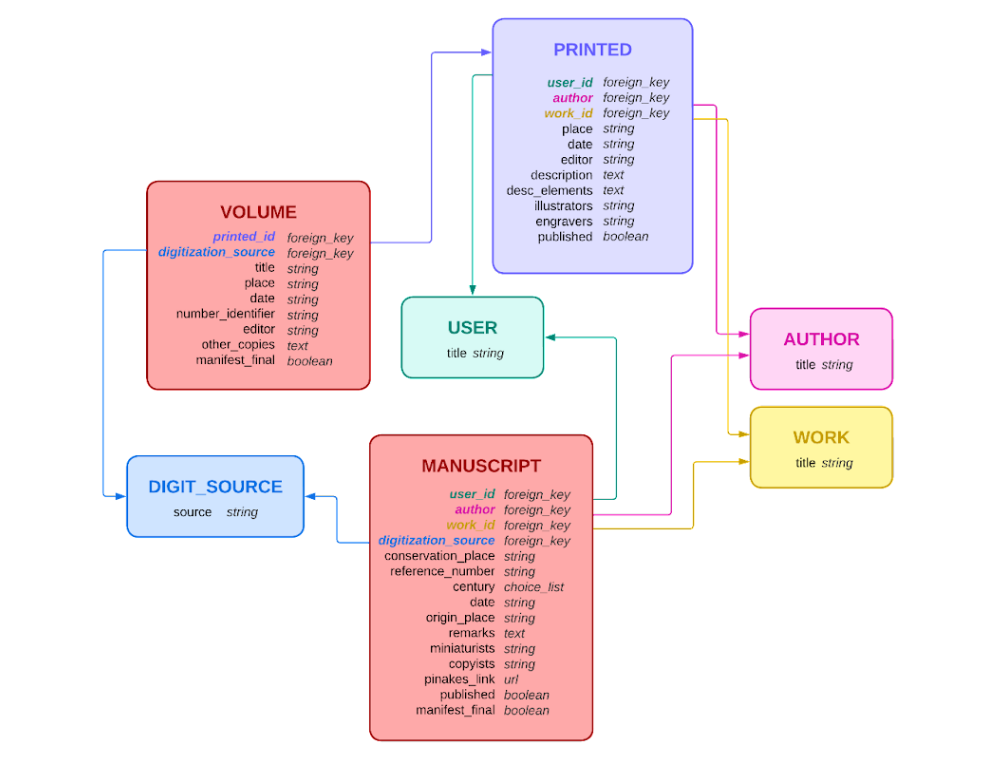
\includegraphics[width=16cm]{images/vhs_data_model.png}
		\caption{Modèle de données de l'application \vhs avant refonte}
		\label{fig:vhs_data_model}
	\end{figure}

\section{Modèle de données de l'application VHS/EIDA}
	\begin{figure}[H]
		\centering
		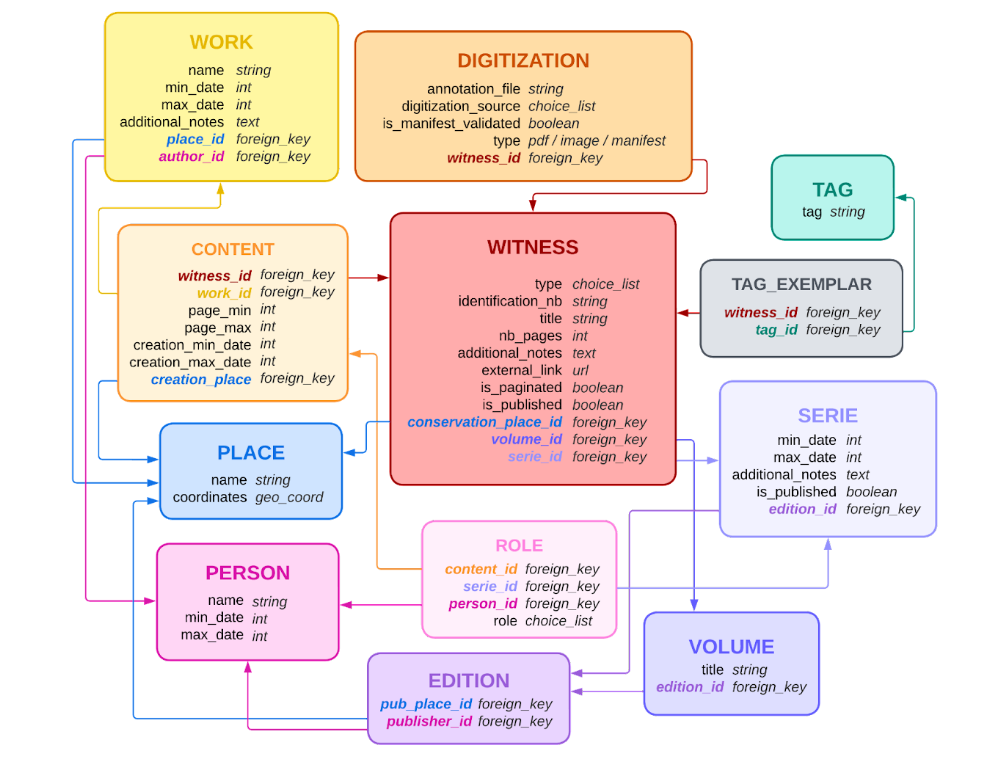
\includegraphics[width=16cm]{images/eida_data_model.png}
		\subcaption{Nouveau modèle de données de l'application \eida appliqué à \vhs}
		\label{fig:eida_data_model}
	\end{figure}
     	\clearemptydoublepage
    \chapter{\label{exapiCahier}extractorAPI : cahier des charges}
	    \section{Fonctionnalités}
L’\api permet de déplacer l’annotation des images envoyées par les utilisateur-rice-s de \eida sur le \gpu : dans une logique de développement modulaire, le modèle entraîné n’est pas intégré directement à l’application, mais dans une \api indépendante. Cette séparation du corps de l’application et du module générant les annotations permet d’éviter le ralentissement général de l’exécution de l’application sur le serveur Web : l’utilisation d’une \api permet de profiter de la capacité de calcul du \gpu lors de l’inférence, alors que l’application est développée sur un serveur différent. La communication en \ssh entre le \gpu et l’application \eida n’étant pas satisfaisante du point de vue de la sécurité, le développement d’une \api permet de gérer ces échanges par une voie sécurisée.

Du point de vue de l’open source, cette forme de développement permet la création d’un outil plus flexible, qui pourra être réutilisé par d’autres projets en fonction de leurs besoins et de leur propre architecture.

L’\api reçoit une requête \http de la part de l’application \eida lorsque l’utilisateur-rice envoie une nouvelle numérisation de son témoin dans la base de données via un formulaire. Le manifeste généré par l’application est envoyé à un \api endpoint qui l’enregistre et en extrait les images, qui sont ensuite traitées par le modèle. Les annotations générées sont retournées à l’application en réponse à la requête, et peuvent ainsi être visualisées par l’utilisateur-rice.

L’objectif d’extractor\api – par rapport à notre \textit{workflow} actuel – est d’automatiser la détection des diagrammes par le modèle, pour que celle-ci puisse être faite à la demande de l’utilisateur-rice, sans intervention humaine, et que les annotations lui soient retournées automatiquement après envoi des numérisations.

	\subsection{\textit{Workflow}}
		\begin{enumerate}
		\item Envoi d’une numérisation par l’utilisateur-rice sur l’application \eida ;
		\item Création automatique d’un manifeste \iiif à partir des images ou du manifeste ;
		\item Envoi du manifeste \iiif via requête \http POST à l’\api endpoint ;
		\item Appel de la fonction Python : 
		\item Vérification et enregistrement du manifeste ;
		\item Enregistrement des images issues du manifeste pour leur traitement (\iiif downloader) ;
		\item Traitement des images par le modèle : création des annotations (fichiers .txt) ;
		\item \textit{Return} : envoi des annotations à l’application ;
		\item Affichage des images annotées à l’utilisateur-rice.
		\end{enumerate}
	
	L’architecture actuelle de l’application implique d’enregistrer deux fois les images : une première fois dans l’application \eida pour générer le manifeste \iiif,  puis une seconde fois sur le \gpu pour lancer l’inférence. On peut envisager le déplacement du serveur Cantaloupe sur le \gpu pour éviter la duplication de cette tâche.

	\subsection{Outils}
	L’\api est développée avec Flask, plus simple et flexible que Django pour la construction d’une \api légère, et le modèle est déployé à l’aide du module PyTorch.

		\subsubsection{Modèle}
		Le modèle utilisé a pour base docExtractor – appuyé sur le réseau de neurones U-Net –, un modèle entraîné sur des images synthétiques de manuscrits générées par l’algorithme SynDoc et sur ImageNet. Le script d’inférence utilisé est celui de YOLOv5.
		Il est nécessaire de prendre en compte, dans le développement de l’\api, que d’autres modèles pour la détection d’objets seront testés, et que sera conservé le modèle produisant les meilleurs résultats. 
		Le modèle final sera un modèle entraîné, idéalement commun avec \vhs. Il est cependant envisageable d’avoir un modèle par type de source (manuscrit ou imprimé), ce qui nécessiterait d'adapter la structure de l'\api pour pouvoir choisir le modèle utilisé en fonction de la requête.
		
		\subsubsection{\textit{Task queues}}
		Pour éviter la surcharge de l’\api et gérer la réception de multiples requêtes, il est nécessaire de mettre en place un task manager comme Celery, qui traite en tâche de fond les requêtes reçues, et permet d’imposer qu’elles soient traitées successivement. 
		
	\subsection{Échange de données}
		\subsubsection{Données envoyées}
		Le manifeste \iiif généré par \eida. 
		S’il est décidé après le réentraînement de conserver un modèle pour chaque type de témoin (manuscrit ou imprimé), il est nécessaire d’envoyer une donnée sur le type de support pour choisir le modèle correspondant.
		\subsubsection{Données reçues}
		Un fichier d’annotations au format \texttt{.txt} par manifeste. Celui-ci contient, pour chaque image :
		\begin{itemize}
			\item le numéro de l’image généré par une fonction \texttt{enumerate()},
			\item le nom du fichier image annoté, 
			\item les coordonnées de la détection au format \texttt{x y width height}.
		\end{itemize}

		Par exemple, pour deux objets détectés sur la 21e image du manuscrit 22 :
		\begin{lstlisting}
			21 ms22_0021.jpg
			514 907 1700 1685
			2424 831 1441 1423\end{lstlisting}

	\subsection{Sécurité}
	Pour assurer la sécurité de l’\api, une authentification avec un token a été envisagée. Pour plus de simplicité, l’\api utilise un décorateur pour \textbf{restreindre les hôtes autorisés} à envoyer des requêtes aux \textit{endpoints} : seuls l’hôte \texttt{obspm.fr} peut envoyer des requêtes pour l’inférence, évitant ainsi un risque de surcharge par des requêtes envoyées depuis un autre hôte.
	
	\subsection{Interactions}
	L’annotation des images est automatique après envoi de la numérisation ; il est cependant nécessaire de prendre en compte le temps de réponse de la requête du point de vue de l’utilisateur-rice.
	 
	L’application \eida répond actuellement à cette problématique en affichant le message flash suivant : “Le processus de conversion de.s fichier.s PDF en images et/ou d'extraction des images à partir de manifeste.s externe.s est en cours. Veuillez patienter quelques instants pour corriger les annotations automatiques.”
	
	On peut envisager de désactiver les boutons de visualisation et d’édition du manifeste jusqu’à réception de la réponse à la requête.

	    \clearemptydoublepage
	\chapter{\label{yoloScript}Script YOLOv5 pour lancer la détection d'objet}
		Le script suivant est une reproduction du script \texttt{detect\_vhs.py} utilisé dans \exapi pour lancer la détection d'objet dans les images envoyées par l'application : \url{https://github.com/jnorindr/extractorAPI/blob/main/yolov5/detect_vhs.py}
		\begin{lstlisting}[language=Python]
	# -*- coding: utf-8 -*-
	# YOLOv5 🚀 by Ultralytics, GPL-3.0 license
	import argparse
	import os
	import platform
	import sys
	from pathlib import Path
	import torch
	
	FILE = Path(__file__).resolve()
	ROOT = FILE.parents[0]  # YOLOv5 root directory
	if str(ROOT) not in sys.path:
	sys.path.append(str(ROOT))  # add ROOT to PATH
	ROOT = Path(os.path.relpath(ROOT, Path.cwd()))  # relative
	
	from models.common import DetectMultiBackend
	from yolov5.utils.dataloaders import IMG_FORMATS, VID_FORMATS, LoadImages, LoadScreenshots, LoadStreams
	from yolov5.utils.general import (Profile, check_file, check_img_size, check_imshow, cv2,
	increment_path, non_max_suppression, scale_boxes, strip_optimizer, xyxy2xywh)
	from yolov5.utils.plots import Annotator, colors, save_one_box
	from yolov5.utils.torch_utils import select_device, smart_inference_mode
	
	
	@smart_inference_mode()
	def run_vhs(
		weights=ROOT / 'yolov5s.pt',  # model path or triton URL
		source=ROOT / 'data/images',  # file/dir/URL/glob/screen/0(webcam)
		data=ROOT / 'data/coco128.yaml',  # dataset.yaml path
		imgsz=(640, 640),  # inference size (height, width)
		conf_thres=0.25,  # confidence threshold
		iou_thres=0.45,  # NMS IOU threshold
		max_det=1000,  # maximum detections per image
		device='',  # cuda device, i.e. 0 or 0,1,2,3 or cpu
		view_img=False,  # show results
		save_txt=False,  # save results to *.txt
		save_conf=False,  # save confidences in --save-txt labels
		save_crop=False,  # save cropped prediction boxes
		nosave=False,  # do not save images/videos
		classes=None,  # filter by class: --class 0, or --class 0 2 3
		agnostic_nms=False,  # class-agnostic NMS
		augment=False,  # augmented inference
		visualize=False,  # visualize features
		update=False,  # update all models
		project=ROOT / 'runs/detect',  # save results to project/name
		name='exp',  # save results to project/name
		exist_ok=False,  # existing project/name ok, do not increment
		line_thickness=3,  # bounding box thickness (pixels)
		hide_labels=False,  # hide labels
		hide_conf=False,  # hide confidences
		half=False,  # use FP16 half-precision inference
		dnn=False,  # use OpenCV DNN for ONNX inference
		vid_stride=1,  # video frame-rate stride
		anno_file="annotation.txt",  # annotation in which write the output
		img_nb=1  # increment of the image
	):
		source = str(source)
		save_img = not nosave and not source.endswith('.txt')  # save inference images
		is_file = Path(source).suffix[1:] in (IMG_FORMATS + VID_FORMATS)
		is_url = source.lower().startswith(('rtsp://', 'rtmp://', 'http://', 'https://'))
		webcam = source.isnumeric() or source.endswith('.txt') or (is_url and not is_file)
		screenshot = source.lower().startswith('screen')
		if is_url and is_file:
			source = check_file(source)  # download
	
		# Directories
		save_dir = increment_path(Path(project) / name, exist_ok=exist_ok)  # increment run
		# (save_dir / 'labels' if save_txt else save_dir).mkdir(parents=True, exist_ok=True)  # make dir
		
		# Load model
		device = select_device(device)
		model = DetectMultiBackend(weights, device=device, dnn=dnn, data=data, fp16=half)
		stride, names, pt = model.stride, model.names, model.pt
		imgsz = check_img_size(imgsz, s=stride)  # check image size
		
		# Dataloader
		bs = 1  # batch_size
		if webcam:
			view_img = check_imshow(warn=True)
			dataset = LoadStreams(source, img_size=imgsz, stride=stride, auto=pt, vid_stride=vid_stride)
			bs = len(dataset)
		elif screenshot:
			dataset = LoadScreenshots(source, img_size=imgsz, stride=stride, auto=pt)
		else:
			dataset = LoadImages(source, img_size=imgsz, stride=stride, auto=pt, vid_stride=vid_stride)
		vid_path, vid_writer = [None] * bs, [None] * bs
		
		# Run inference
		model.warmup(imgsz=(1 if pt or model.triton else bs, 3, *imgsz))  # warmup
		seen, windows, dt = 0, [], (Profile(), Profile(), Profile())
		for i, (path, im, im0s, vid_cap, s) in enumerate(dataset, start=1):
			with open(anno_file, 'a') as f:
				f.write(f"{img_nb} {path.split('/')[-1]}\n")  # write canvas and image name
			with dt[0]:
				im = torch.from_numpy(im).to(model.device)
				im = im.half() if model.fp16 else im.float()  # uint8 to fp16/32
				im /= 255  # 0 - 255 to 0.0 - 1.0
				if len(im.shape) == 3:
					im = im[None]  # expand for batch dim
	
		# Inference
		with dt[1]:
			visualize = increment_path(save_dir / Path(path).stem, mkdir=True) if visualize else False
			pred = model(im, augment=augment, visualize=visualize)
	
		# NMS
		with dt[2]:
			pred = non_max_suppression(pred, conf_thres, iou_thres, classes, agnostic_nms, max_det=max_det)
	
		# Second-stage classifier (optional)
		# pred = utils.general.apply_classifier(pred, classifier_model, im, im0s)
		
		# Process predictions
		for i, det in enumerate(pred):  # per image
			seen += 1
			if webcam:  # batch_size >= 1
				p, im0, frame = path[i], im0s[i].copy(), dataset.count
				s += f'{i}: '
			else:
				p, im0, frame = path, im0s.copy(), getattr(dataset, 'frame', 0)
	
			p = Path(p)  # to Path
			save_path = str(save_dir / p.name)  # im.jpg
			txt_path = str(save_dir / 'labels' / p.stem) + ('' if dataset.mode == 'image' else f'_{frame}')  # im.txt
			s += '%gx%g ' % im.shape[2:]  # print string
			gn = torch.tensor(im0.shape)[[1, 0, 1, 0]]  # normalization gain whwh
			imc = im0.copy() if save_crop else im0  # for save_crop
			annotator = Annotator(im0, line_width=line_thickness, example=str(names))
			if len(det):
				# Rescale boxes from img_size to im0 size
				det[:, :4] = scale_boxes(im.shape[2:], det[:, :4], im0.shape).round()
	
				# Print results
				for c in det[:, 5].unique():
					n = (det[:, 5] == c).sum()  # detections per class
					s += f"{n} {names[int(c)]}{'s' * (n > 1)}, "  # add to string
	
				# Write results
				for *xyxy, conf, cls in reversed(det):
					x, y, width, height = int(xyxy[0]), int(xyxy[1]), int(xyxy[2]-xyxy[0]), int(xyxy[3]-xyxy[1])
					with open(anno_file, 'a') as f:
						f.write(f'{x} {y} {width} {height}\n')  # write image coordinates
					if save_txt:  # Write to file
						xywh = (xyxy2xywh(torch.tensor(xyxy).view(1, 4)) / gn).view(-1).tolist()  # normalized xywh
						line = (cls, *xywh, conf) if save_conf else (cls, *xywh)  # label format
						with open(f'{txt_path}.txt', 'a') as f:
							f.write(('%g ' * len(line)).rstrip() % line + '\n')
	
					if save_img or save_crop or view_img:  # Add bbox to image
						c = int(cls)  # integer class
						label = None if hide_labels else (names[c] if hide_conf else f'{names[c]} {conf:.2f}')
						annotator.box_label(xyxy, label, color=colors(c, True))
					if save_crop:
						save_one_box(xyxy, imc, file=save_dir / 'crops' / names[c] / f'{p.stem}.jpg', BGR=True)
	
			# Stream results
			im0 = annotator.result()
			if view_img:
				if platform.system() == 'Linux' and p not in windows:
					windows.append(p)
					cv2.namedWindow(str(p), cv2.WINDOW_NORMAL | cv2.WINDOW_KEEPRATIO)  # allow window resize (Linux)
					cv2.resizeWindow(str(p), im0.shape[1], im0.shape[0])
				cv2.imshow(str(p), im0)
				cv2.waitKey(1)  # 1 millisecond
	
			# Save results (image with detections)
			if save_img:
				if dataset.mode == 'image':
					cv2.imwrite(save_path, im0)
				else:  # 'video' or 'stream'
					if vid_path[i] != save_path:  # new video
						vid_path[i] = save_path
						if isinstance(vid_writer[i], cv2.VideoWriter):
							vid_writer[i].release()  # release previous video writer
						if vid_cap:  # video
							fps = vid_cap.get(cv2.CAP_PROP_FPS)
							w = int(vid_cap.get(cv2.CAP_PROP_FRAME_WIDTH))
							h = int(vid_cap.get(cv2.CAP_PROP_FRAME_HEIGHT))
						else:  # stream
							fps, w, h = 30, im0.shape[1], im0.shape[0]
						save_path = str(Path(save_path).with_suffix('.mp4'))  # force *.mp4 suffix on results videos
						vid_writer[i] = cv2.VideoWriter(save_path, cv2.VideoWriter_fourcc(*'mp4v'), fps, (w, h))
					vid_writer[i].write(im0)
			
		if update:
			strip_optimizer(weights[0])  # update model (to fix SourceChangeWarning)
\end{lstlisting}
	    \clearemptydoublepage
	\chapter{\label{DHSeminar}DH Seminar: extractorAPI}
		La présentation suivante constitue le support d'un séminaire d'humanités numériques donné le 13 juin 2023 en présence de l'équipe du projet \eida. Le séminaire visait à présenter l'\api développée dans le cadre du stage.
		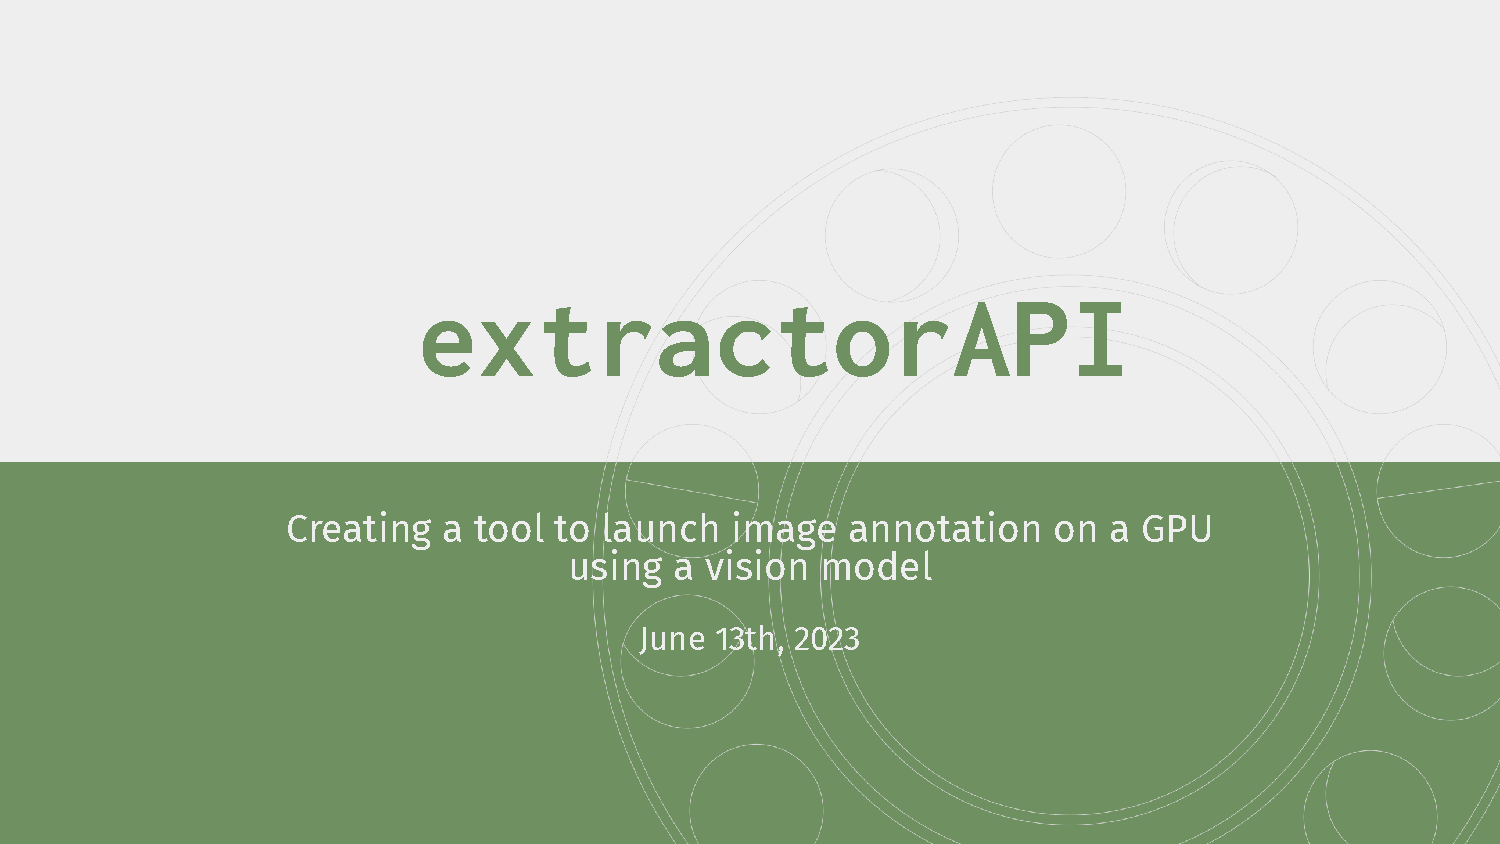
\includepdf[nup=1x2,pages=-, scale=0.8, delta=0 10mm]{templates/annexes/dhseminar.pdf}
	    \clearemptydoublepage
	\chapter[Annotate images with extractorAPI]{\label{exapiAnno}Annotate images from EiDA with extractorAPI}
		Ce document est extrait du Wiki de l'\api, disponible sur GitHub en accompagnement du code. Il a été rédigé pour documenter les interactions entre \exapi et l'application \eida, pour faciliter la réutilisation de l'\api par des projets tiers. Le document est disponible à l'adresse suivante : \url{https://github.com/jnorindr/extractorAPI/wiki/Annotate-images-from-EiDA-with-extractorAPI}
		\section{Workflow}
	\begin{enumerate}
	\item User submits a witness
	\item Verification: did the user send a digitization?
	\item A flash message informs the user of the delay for receiving the annotations
	\item Images are downloaded and \iiif manifest is generated
	\item POST request is sent from \eida to \exapi with manifest link and type of witness as parameters
	\item \api: images are downloaded, detection is launched and annotation file is generated
	\item POST request is sent from \exapi to \eida with annotation file
	\item Annotations are indexed to be displayed for the user
	\end{enumerate}

\section{Settings}
	\subsection{EiDA}
	In the \texttt{.env} file, the \texttt{EXAPI} variable must be set with the \URL of the \api.
	\begin{lstlisting}
		EXAPI="<gpu-api-address>"\end{lstlisting}
	
	In the settings file \texttt{settings.py}, complete the \texttt{GPU\_PORT} variable so the \texttt{GPU\_URL} variable can be set.
	\begin{lstlisting}
		GPU_PORT = 5000
		GPU_URL = f"{ENV('EXAPI')}:{GPU_PORT}"\end{lstlisting}

	\subsection{extractorAPI}
	In the \texttt{.env} file, set the \texttt{CLIENT\_APP\_URL} variable with the \URL of the app.
	\begin{lstlisting}
		CLIENT_APP_URL="<url>"\end{lstlisting}

\section{Sending for detection}
	\begin{figure}[h]
	\centering
	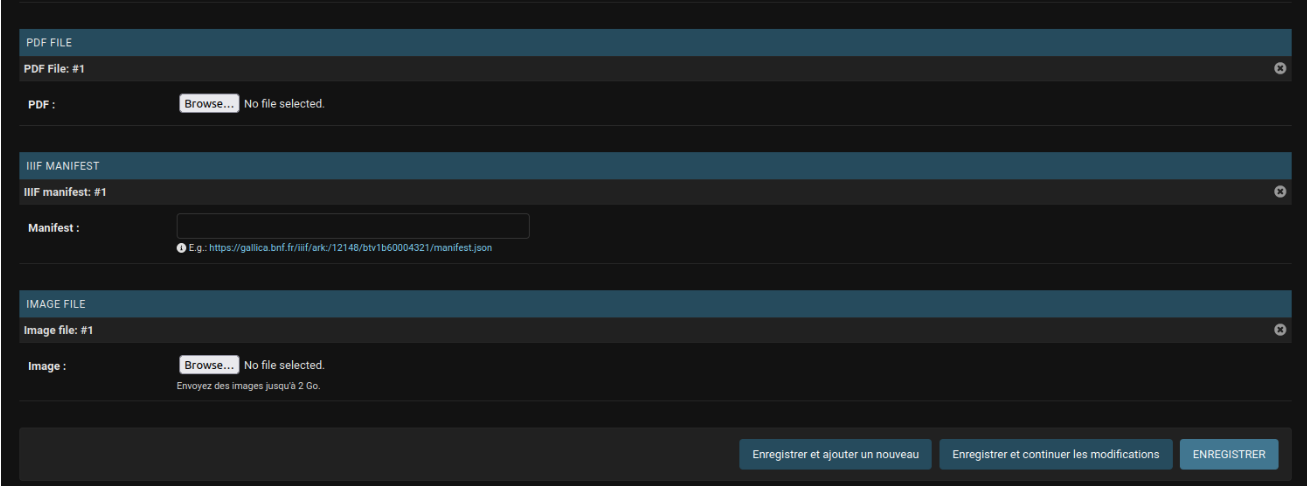
\includegraphics[width=15cm]{images/eida_send_manifest.png}
	\caption{Capture d'écran du formulaire d'envoi d'une numérisation dans l'application \eida}
	\label{fig:eida_send_manifest}
	\end{figure}

	\subsection{IIIF manifest}
	The user creates a \textbf{witness}, fills in the form and submit a digitization (either a PDF file, a \iiif manifest or images).

	The images are downloaded and the \textbf{\eida \iiif manifest} is generated: the request to the \api is not sent until all of the images are downloaded, to avoid errors and annotation of incomplete manifests.

	\subsection{annotate\_wit function}
	To send requests to \exapi from the \eida application, we created a function in \texttt{vhs-platform/vhsapp/utils/iiif/annotation.py}. The function sends a \textbf{POST request} to the \api endpoint \texttt{/run\_detect}, which launches detection on the images from the digitization.
	
	The request takes as arguments the \textbf{\URL of the manifest} we want annotated, and the \textbf{abbreviation} of the witness type.
	
	The \texttt{event} argument is used with the method \texttt{.wait()} to ensure the function \textbf{waits for an event to be set} before sending the request to the \api – this event will be set when the images from the previous step are all downloaded.
	
	\begin{lstlisting}[language=Python]
	def annotate_wit(event, witness_id, wit_abbr=MS_ABBR, version=MANIFEST_AUTO):
		wit_type = MS if wit_abbr == MS_ABBR else VOL
		api_endpoint = f"{GPU_URL}/run_detect"
	
		manifest_url = (
			f"{VHS_APP_URL}/{APP_NAME}/iiif/{version}/{wit_type}/{witness_id}/manifest.json"
		)
		data = {"manifest_url": manifest_url, "wit_abbr": wit_abbr}
	
		event.wait()
		requests.post(url=api_endpoint, data=data)
		
		return print(f"Witness {witness_id} sent for diagram extraction")\end{lstlisting}
	
	\subsection{Automating the annotation request}
	To launch annotation automatically after the user submits a digitization, we added a \textbf{background task} to the save method of \texttt{Manifests}, \texttt{Pdf} and \texttt{Image} objects.
	
	We use \textbf{threading} to avoid an interruption of the other tasks of the app while waiting for a response to the request.

		\subsubsection{User submitted a IIIF manifest}
		For manifests, we modified the save method of the \texttt{ManifestManuscript} and the \texttt{ManifestVolume} classes in \texttt{vhs/vhs-platform/vhsapp/models/digitization.py}. Ideally, we would have a unique save method for both types.
		
		An \texttt{event} object is created and can be passed through the various \textbf{threads}: the first thread \texttt{t} calls the function \texttt{extract\_images\_from\_iiif\_manifest} (in \texttt{vhs/vhs-platform/ vhsapp/utils/iiif/download.py}) to download images and \textbf{set the event} when the function is done running.

		\begin{lstlisting}[language=Python]
	def extract_images_from_iiif_manifest(manifest_url, witness_ref, event):
		"""
		Extract all images from an IIIF manifest
		"""
		downloader = IIIFDownloader(manifest_url, witness_ref)
		downloader.run()
		event.set()\end{lstlisting}

		\texttt{event.set()} returns a boolean value: event is \texttt{True} when the function has \textbf{run to its completion}. Because we used an \texttt{event.wait()} in the \texttt{annotate\_wit} function, it cannot run unless this value is \texttt{True}.
		
		When the image extraction is done and the event is set, the thread \texttt{t2} starts, therefore \textbf{sending the newly generated manifest to the \api for annotation}.

		\begin{lstlisting}[language=Python]
	class ManifestManuscript(Manifest):
		manuscript = models.ForeignKey(Manuscript, on_delete=models.CASCADE)
		
		def save(self, *args, **kwargs):
			# Call the parent save method to save the model
			super().save(*args, **kwargs)
			
			event = threading.Event()
		
			# Run the async extraction of images from an IIIF manifest in the background using threading
			t = threading.Thread(
				target=extract_images_from_iiif_manifest,
				args=(
					self.manifest,
					f"{MS_ABBR}{self.manuscript.id}",
					event,
				),
			)
			t.start()
			
			t2 = threading.Thread(
				target=annotate_wit,
				args=(
					event,
					f"{self.manuscript.id}",
					f"{MS_ABBR}",
				),
			)
			t2.start()\end{lstlisting}
	
		\subsubsection{User submitted a PDF file}
		For PDF files, the process is the same as for manifests.
		The \texttt{event} is set at the end of the \texttt{pdf\_to\_img function}, when all pages are converted to images, in \texttt{vhs/vhs-platform/ vhsapp/utils/functions.py}.

		\begin{lstlisting}[language=Python]
	def pdf_to_img(event, pdf_name):
		"""
		Convert the PDF file to JPEG images
		"""
		pdf_path = f"{BASE_DIR}/{MEDIA_PATH}/{pdf_name}"
		
		# e.g. pdf_name = "volumes/pdf/filename.pdf" => "filename"
		pdf_name = pdf_path.split("/")[-1].split(".")[0]
		pdf_info = pdfinfo_from_path(pdf_path, userpw=None, poppler_path=None)
		page_nb = pdf_info["Pages"]
		step = 2
		try:
			for img_nb in range(1, page_nb + 1, step):
				batch_pages = convert_from_path(
				pdf_path,
				dpi=300,
				first_page=img_nb,
				last_page=min(img_nb + step - 1, page_nb),
				)
				for page in batch_pages:
					save_img(page, f"{pdf_name}_{img_nb:04d}.jpg")
					img_nb += 1
			event.set()
		except Exception as e:
			log(f"[pdf_to_img] Failed to convert {pdf_name}.pdf to images:\n{e}")\end{lstlisting}

		In \texttt{vhs/vhs-platform/vhsapp/models/digitization.py}, the \texttt{save} method of the \texttt{Pdf} class was modified to start a second thread when the function has run.
		
		\begin{lstlisting}[language=Python]
	class Pdf(Digitization):
		class Meta:
			verbose_name = "PDF File"
			verbose_name_plural = "PDF Files"
			abstract = True  # TODO: make this class not abstract
		
		def __str__(self):
			return self.pdf.name
		
		def save(self, *args, **kwargs):
			# Call the parent save method to save the model
			super().save(*args, **kwargs)
			# Run the PDF to image async conversion task in the background using threading
			# t = threading.Thread(target=self.to_img())
	
			event = threading.Event()
			
			t = threading.Thread(target=pdf_to_img, args=(event, f"{self.pdf.name}",))
			t.start()
		
			t2 = threading.Thread(
				target=annotate_wit,
				args=(
					event,
					f"{self.volume.id if 'vol' in self.pdf.name else self.manuscript.id}",
					f"{VOL_ABBR if 'vol' in self.pdf.name else MS_ABBR}",
				),
			)
			t2.start()\end{lstlisting}

		\subsubsection{User submitted images}
		\begin{lstlisting}[language=Python]
	def save(self, *args, **kwargs):
		if self.image:
			img = Image.open(self.image)
			# Check if the image format is not JPEG
			if img.format != "JPEG":
				# Convert the image to JPEG format
				self.image = convert_to_jpeg(self.image)
		# Call the parent save method to save the model
		super().save(*args, **kwargs)
		
		event = threading.Event()
	
		t = threading.Thread(
			target=annotate_wit,
			args=(
				event,
				f"{self.volume.id if 'vol' in self.image.name else self.manuscript.id}",
				f"{VOL_ABBR if 'vol' in self.image.name else MS_ABBR}",
			),
		)
		t.start()\end{lstlisting}
		
\section{Receiving annotations}
For the annotations to be returned \textbf{from \exapi to the \eida application} after detection, we create an \textbf{endpoint} in \texttt{vhs/vhs-platform/vhs/urls.py}.

\begin{lstlisting}[language=Python]
	path(
		f"{APP_NAME}/<str:wit_type>/<int:wit_id>/annotate/",
		receive_anno,
		name="receive-annotations",
	),\end{lstlisting}

The endpoint calls the function \texttt{receive\_anno} in \texttt{vhs/vhs-platform/vhsapp/utils/ views.py} which receives a \textbf{file} from a \textbf{POST request from \exapi}. When the file is received, \textbf{if it is a text file}, its content is \textbf{written in a file in the annotation directory}. If the file already exists, the content is rewritten.

When the annotation file is saved, the annotations are indexed by the function \texttt{index\_anno}. 

\begin{lstlisting}[language=Python]
	def receive_anno(request, wit_id, wit_type):
		if request.method == "POST":
			annotation_file = request.FILES["annotation_file"]
			file_content = annotation_file.read()
		
			if is_text_file(file_content):
				anno_path = f"{BASE_DIR}/{MEDIA_PATH}/{MS_ANNO_PATH if wit_type == 'manuscript' else VOL_ANNO_PATH}"
				
				try:
					with open(f"{anno_path}/{wit_id}.txt", "w+b") as f:
						f.write(file_content)
		
				except Exception as e:
					log(f"[receive_anno] Failed to open received annotations for {wit_type} #{wit_id}: {e}")
		
				manifest_url = (f"{VHS_APP_URL}/{APP_NAME}/iiif/v2/{wit_type}/{wit_id}/manifest.json")
				try:
					index_anno(manifest_url, wit_type, wit_id)
				except Exception as e:
					log(f"[receive_anno] Failed to index annotations for {wit_type} #{wit_id}: {e}")
					
				return JsonResponse({"message": "Annotation received and indexed."})
			else:
				return JsonResponse({"message": "Invalid request. File is not a text file."}, status=400)
		else:
			return JsonResponse({"message": "Invalid request."}, status=400)\end{lstlisting}

\section{Indexing annotations}
In \texttt{vhs/vhs-platform/vhsapp/utils/iiif/annotation.py}, the function \texttt{index\_anno} launches the indexation of the annotations, to go \textbf{from a \texttt{.txt} file to an annotated manifest}. 
A \textbf{GET request} is sent to retrieve the \json content of the manifest, which is sent to the \textbf{annotation server} through a \textbf{POST request}. 

\begin{lstlisting}[language=Python]
	def index_anno(manifest_url, wit_type, wit_id):
		try:
			manifest = requests.get(manifest_url)
			manifest_content = manifest.json()
		except Exception as e:
			log(f"[index_anno]: Failed to load manifest for {wit_type} n°{wit_id}: {e}")
	
		requests.post(f"{SAS_APP_URL}/manifests", json=manifest_content)
	
		try:
			requests.get(f"{VHS_APP_URL}/{APP_NAME}/iiif/v2/{wit_type}/{wit_id}/populate/")
		except Exception as e:
			log(f"[index_anno]: Failed to index {wit_type} n°{wit_id}: {e}")\end{lstlisting}

		\clearemptydoublepage

\backmatter
    \printacronyms[title=Liste des acronymes,toctitle=Acronymes]
    \printglossary
    \listoffigures
    \clearemptydoublepage
    \tableofcontents
\end{document}